
\documentclass[11pt]{article}

% ================================================================
% Packages and page style
% ================================================================
\usepackage[margin=0.72in]{geometry}
\usepackage[T1]{fontenc}
\usepackage[utf8]{inputenc}
\usepackage{lmodern}
\usepackage{microtype}
\usepackage{amsmath,amssymb,mathtools}
\usepackage{booktabs,longtable,tabularx,array}
\usepackage{graphicx}
\usepackage{xcolor}
\usepackage[normalem]{ulem}
\usepackage[colorinlistoftodos,textsize=small]{todonotes}
\usepackage{hyperref}

% ================================================================
% Revision markup for this advisor-facing update
% ================================================================
\newcommand{\oldtxt}[1]{\textcolor{blue!70!black}{\sout{#1}}}
\newcommand{\newtxt}[1]{\textcolor{green!45!black}{#1}}
\newcommand{\latesttxt}[1]{\textcolor{purple!85!black}{#1}}

\hypersetup{
  colorlinks=true,
  linkcolor=black,
  citecolor=blue!55!black,
  urlcolor=blue!65!black
}
\makeatletter
\g@addto@macro\UrlBreaks{\do\-\do\_\do:\do~\do.}
\makeatother

\setlength{\parindent}{0pt}
\setlength{\parskip}{4.5pt}
\renewcommand{\arraystretch}{1.10}
\newcolumntype{Y}{>{\raggedright\arraybackslash}X}

% ================================================================
% Baseline metadata -- current public v2 baseline + generated Prineville registries
% ================================================================
\newcommand{\BaselineName}{\oldtxt{Prineville Public-Data Baseline v1}\ \latesttxt{Prineville Public-Data Baseline v2 --- City utility-meter integration}}
\newcommand{\BaselineCommit}{\oldtxt{\texttt{ac0adf6}}\ \oldtxt{current public \texttt{main}; use git history for the exact snapshot hash}\ \latesttxt{public \texttt{main} at \texttt{08b0c112d8883eb4d23bb05d0d40e1a42c863593}}}
\newcommand{\SourceCount}{\oldtxt{44}\latesttxt{50}}
\newcommand{\QuantityCount}{\oldtxt{76}\latesttxt{82}}
\newcommand{\ModelCount}{\oldtxt{18}\latesttxt{26}}

% ================================================================
% Provenance vocabulary
% ================================================================
\newcommand{\Reported}{\textsc{reported}}
\newcommand{\Measured}{\textsc{measured}}
\newcommand{\Derived}{\textsc{derived}}
\newcommand{\Fitted}{\textsc{fitted}}
\newcommand{\Proxy}{\textsc{proxy}}
\newcommand{\Scenario}{\textsc{scenario}}
\newcommand{\Benchmark}{\textsc{external benchmark}}
\newcommand{\NotIdentified}{\textsc{not identified}}
\newcommand{\NotNecessary}{\textsc{not necessary}}

\newcommand{\mthree}{\mathrm{m}^3}
\newcommand{\COtwo}{\mathrm{CO}_2}

% Use existing figure if present; otherwise compile with a visible placeholder.
\newcommand{\maybegraphic}[3][0.94\linewidth]{%
\begin{figure}[ht]
\centering
\IfFileExists{#2}{
  \includegraphics[width=#1]{#2}
}{
  \fbox{\parbox[c][1.25in][c]{0.90\linewidth}{\centering
  \textbf{Figure placeholder}\\[3pt]#3\\[3pt]\texttt{#2}}}
}
\caption{#3}
\end{figure}
}

\title{\oldtxt{\textbf{From Public Data to a Coupled}}\ \oldtxt{\textbf{Data-Center Energy--Water Model}}\\
\latesttxt{\textbf{From Public Data to Network-Based}}\\
\latesttxt{\textbf{Data-Center Planning}}\\
\large \oldtxt{Meta Prineville as an Empirical Test Bed}\\
\large \oldtxt{Prineville Site Test Bed + M100 External Facility-Model Benchmark}\\
\large \newtxt{Prineville Site Test Bed + External Facility-Model Validation}\\
\large \latesttxt{Facility Energy, Water Sources, Groundwater Response, and Decision Validation}}
\author{}
\date{\oldtxt{Prineville Public-Data Baseline v1}\\[-0.15em]
\latesttxt{Prineville Public-Data Baseline v2 --- City utility-meter integration}}

\begin{document}
\maketitle
\vspace{-0.9em}

{\small
\textit{Revision markup: }
\newtxt{green = prior external-validation revision};
\latesttxt{purple = September 3, 2026 project-status synchronization};
\oldtxt{blue strikeout = superseded wording}.
\todo[inline]{Short TODOs mark remaining identification or implementation tasks; they are not established results.}
}

{\small \oldtxt{Current public \texttt{main} reports Prineville Public-Data Baseline v2. The generated Prineville report lists 50 sources, 82 quantities, and 26 registered methods/models; the validated City-integration run reported 126 package tests PASS. Exact snapshot provenance should be taken from git history and the generated registries rather than from a hard-coded hash in this glossary.} \latesttxt{This refresh is pinned to public \texttt{main} at \texttt{08b0c112d8883eb4d23bb05d0d40e1a42c863593}. Deterministic reporting regenerated the authoritative 50-source, 82-quantity, and 26-method/model registries byte-for-byte; external validation streams remain outside the Prineville site-source count.}}

\begin{center}
\small
% \textit{Goal for this meeting: understand the big modeling idea, the evidence that currently supports each link, what is reconstructed rather than observed, what has worked or failed, and the next identification step.}
\end{center}

% ================================================================
\section{Big picture: what are we ultimately trying to model?}
% ================================================================

The long-run research objective is to connect a data center's operation to the physical systems that bear its environmental impacts:
\[
\boxed{\parbox{0.92\linewidth}{\centering
workload
\(\rightarrow\)
IT power / heat
\(\rightarrow\)
facility cooling and power
\(\rightarrow\)
\{grid, direct water\}
\(\rightarrow\)
\{emissions / generator water, water-system / groundwater state\}
\(\rightarrow\)
operations, siting, and policy.}}
\]

The literature contains strong models for many individual links, but the links are usually studied separately. Operational papers often treat carbon or water intensity as exogenous signals; siting models often use static regional water coefficients; groundwater models take pumping schedules as given. The opportunity is to connect these layers while keeping the physical and accounting boundaries explicit.

\latesttxt{The flagship validation is consequently a planning comparison rather than a facility-fit competition:}
\[
{\color{purple!85!black}
\begin{aligned}
M_0 &: \ \text{static PSCC-style environmental coefficients},\\
M_1 &: \ \text{validated facility/source/groundwater consequences}.
\end{aligned}
}
\]
\latesttxt{The central question is whether the richer physical representation changes siting, technology/source choice, groundwater constraints, equity outcomes, or regret.}

\oldtxt{\textbf{Prineville is the empirical test bed.} The present project asks how much of this full chain can be populated, reconstructed, and validated from public data for one real hyperscale campus before moving to coupled optimization.}

\oldtxt{Previous framing: Prineville site evidence + M100 as the only external facility benchmark.}

{\small
\oldtxt{\textbf{Prineville remains the site-specific test bed;}} \oldtxt{\textbf{the internal facility model is now validated}}\\
\oldtxt{\textbf{through a complementary external stack}} \oldtxt{\textbf{rather than a single site.}}\\
\oldtxt{M100 provides measured facility-structure evidence;} \oldtxt{Lei--Masanet provides climate--technology PUE/WUE physics}\\
\oldtxt{and archetypes;} \oldtxt{Frontier provides independent measured power/thermal evidence.}\\
\oldtxt{These sources constrain model form,} \oldtxt{while Prineville remains the site-specific}\\
\oldtxt{electricity/water/grid/groundwater case.}\par}

\latesttxt{\textbf{Prineville remains the integrated site-specific test bed, while external experiments constrain model structure rather than supply a universal quantitative facility model.} M100 is a frozen structural benchmark; Frontier provides closed independent evidence that IT load affects accessory power; ESIF adds measured evidence that facility overhead can change across architecture/operating regimes; Lei--Masanet remains useful for climate--technology and conditioning-water structure but its final quantitative adapter promotion is blocked; and Forest City v3 supports qualitative physical transportability while explicitly not validating numerical transfer. The facility layer is therefore substantially de-risked structurally, but site/archetype coefficients remain uncertain.}

\subsection*{One view of the full model and current Prineville status}

\begingroup
\small
\begin{longtable}{@{}p{0.18\linewidth}p{0.22\linewidth}p{0.17\linewidth}p{0.35\linewidth}@{}}
\caption{\latesttxt{One view of the full model and current Prineville status. Statuses apply only at the stated physical/accounting boundary.}}\\
\toprule
\textbf{Layer} & \textbf{Main quantity} & \textbf{Current status} & \textbf{What that means in Prineville} \\
\midrule
\endfirsthead
\toprule
\textbf{Layer} & \textbf{Main quantity} & \textbf{Current status} & \textbf{What that means in Prineville} \\
\midrule
\endhead
Workload & jobs / utilization \(x_t,u_t\) & \Scenario & No public Meta workload telemetry; current workload paths are synthetic. \\
IT power & \(P^{IT}_t\) & \Fitted / \Scenario & Latent hourly shape; constrained indirectly by annual facility electricity. \\
\latesttxt{Modern AI compute power} & \latesttxt{\(P^{compute}_{w,N,t}\)} & \latesttxt{frozen bounded external evidence} & \latesttxt{Controlled CPU/H100 compute-component energy is workload/mode/scale conditioned; full-node AC, other-node power, production mix, and the node-to-facility-IT bridge remain incomplete.} \\
\newtxt{External facility structure} & \newtxt{\(P^{IT}_t,P^{cool}_t,P^{fac}_t\)} & \newtxt{\Benchmark} & \newtxt{M100 Apr--Dec 2021 telemetry validates model structure and boundaries, not Prineville/generic coefficients.} \\
\oldtxt{Facility energy--water archetypes} & \oldtxt{\(PUE_k(\mathbf w),WUE_k(\mathbf w)\)} & \oldtxt{external benchmark / validation in progress} & \oldtxt{Lei--Masanet first audit/reproduction identifies an IT-normalized climate--technology intensity model; publication-scale annual reproduction and RNG gates are currently running.} \\
\latesttxt{Facility energy--water archetype structure} & \latesttxt{\(PUE_k(\mathbf w),\)}\newline\latesttxt{\(WUE_k(\mathbf w),W^{cond}\)} & \latesttxt{external benchmark; PARTIAL / closed} & \latesttxt{Lei--Masanet strongly supports climate--technology intensity structure and conditioning-water components, but the final reproducibility closure is PARTIAL and quantitative adapter promotion is blocked.} \\
\latesttxt{Facility overhead regime/state} & \latesttxt{\(P^{overhead}_t,A^{arch}_t,S^{op}_t\)} & \latesttxt{external benchmark; PARTIAL / closed} & \latesttxt{ESIF shows that a stationary IT+weather model is insufficient for total auxiliary power across a late operating/infrastructure regime shift; use structure, not ESIF coefficients.} \\
Facility electricity & \(E^{fac}_y\) & \Reported & Annual Meta campus electricity is high-confidence ground truth. \\
Cooling & \(Q^{cool}_t,P^{cool}_t\) & \Derived & Simplified gray-box physics driven by IT load, weather, and assumed parameters. \\
Weather & \(T,T_d,T_{wb},p\) & \Measured / \Derived & \oldtxt{NOAA KS39/KRDM observations; wet bulb derived psychrometrically.} \latesttxt{Canonical hierarchy is KS39 when QC-usable, KRDM observational fallback, then bias-adjusted KBDN as tertiary observational fallback; RH/wet bulb are recomputed after the final mixed-source selection.} \\
Campus water & \(W^{Meta}_y\) & \Reported & Annual Meta withdrawal is reported for 2014--2024. It is withdrawal, not consumption. \\
\oldtxt{Subannual campus water} & \oldtxt{\(W_t\)} & \oldtxt{scenario / weak prediction} & \oldtxt{No monthly campus meter; current allocations/predictions are not telemetry.} \\
\latesttxt{City customer-service water} & \latesttxt{\(W^{City,service}_m\)} & \latesttxt{\Reported\ (observed meter report)} & \latesttxt{Monthly Facebook Data Center WATER-COMM + ADD'L WATER customer-service component is observed for 2012--2026 (2026 through July); it is not total Meta campus withdrawal.} \\
\latesttxt{All-source monthly campus withdrawal} & \latesttxt{\(W^{Meta,total}_m\)} & \latesttxt{\NotIdentified} & \latesttxt{Bulk/hydrant, SWR, WELL-METER-FOR-SEW, Trailer City, Warehouse, direct POD, reuse/return/storage, and parent/submeter semantics prevent a closed monthly campus balance.} \\
Regional grid demand & \(D^{PACW}_t\) & \Measured / \Proxy & EIA-930 when available; FERC-constrained proxy for earlier years. \\
Grid carbon & \(CI_t\) & \Derived / \Proxy & Regional average/accounting context; not Meta-specific marginal emissions. \\
Generator water/emissions & \(W_{g,t},CO_{2,g,t}\) & \Reported / \Derived & Strong plant context; no claim that particular plants physically serve Meta. \\
Water-system pumping & \(Q_{i,t}\) & \Reported & OWRD municipal/direct-POD pumping at specific reporting boundaries. \\
GWIS groundwater level & \(BLS_{i,t}\) (and reported AMSL) & \Measured, QC-qualified & Individual-well observations; measurement-condition uncertainty remains. \\
Within-well relative head & \(\tilde h_{i,t}=-(BLS_{i,t}-\overline{BLS}_i)\) & \Derived & Physically signed within-well anomaly used for the planned empirical benchmark; not a spatial groundwater-state field. \\
Groundwater response / state model & pumping \(\rightarrow \tilde h\); future \(h_{n,t}\) & \NotIdentified & Next experiment tests whether antecedent pumping predicts within-well anomalies; a common-datum/network state is not identified. \\
Optimization & workload/siting/source choice & \NotIdentified & Future layer; response functions and costs are not yet sufficiently identified. \\
\bottomrule
\end{longtable}
\endgroup

% ================================================================
\section{Evidence stack: who provides the data, and what boundary do they observe?}
% ================================================================

The strongest feature of the pipeline is that it does \emph{not} treat all public data as if they measured the same thing. Different authorities observe different physical or accounting boundaries.

\begingroup
\small
\begin{longtable}{@{}p{0.15\linewidth}p{0.20\linewidth}p{0.23\linewidth}p{0.34\linewidth}@{}}
\caption{\latesttxt{Authority/evidence stack. Each row identifies the physical or accounting boundary contributed by that source; rows are not interchangeable measurements.}}\\
\toprule
\textbf{Authority / entity} & \textbf{What it is} & \textbf{What we use} & \textbf{Boundary / why it matters} \\
\midrule
\endfirsthead
\toprule
\textbf{Authority / entity} & \textbf{What it is} & \textbf{What we use} & \textbf{Boundary / why it matters} \\
\midrule
\endhead
Meta & Data-center operator & Annual Prineville electricity, withdrawal, location-based Scope 2, selected site/design disclosures & \oldtxt{Campus-level ground truth; no public hourly IT or customer-meter telemetry.} \latesttxt{High-confidence annual reporting boundary; no public hourly IT telemetry. Exact PRN-only versus PRN+CCO inclusion by reporting vintage remains unresolved.} \\
\newtxt{CINECA / M100 ExaData \cite{m100exadata}} & \newtxt{External measured Tier-0 facility benchmark} & \newtxt{Facility/IT power, cooling components/state, node power, liquid thermal telemetry, weather} & \newtxt{Validates generic facility-model structure and boundaries; not Prineville telemetry and not a source of generic coefficients.} \\
\oldtxt{Lei--Masanet \cite{lei2022} + public code} & \oldtxt{Climate/technology facility archetype model} & \oldtxt{Joint PUE/WUE and explicit conditioning-water components across published cooling cases} & \oldtxt{Used as an intensity/archetype backbone; annual reproduction is gated before project translation. It does not identify source withdrawal or groundwater pumping.} \\
\latesttxt{Lei--Masanet \cite{lei2022} + public code} & \latesttxt{Climate/technology facility archetype evidence} & \latesttxt{PUE/WUE intensity structure and conditioning-water components} & \latesttxt{Final reproducibility disposition PARTIAL; adapter promotion NO/blocked. Retain qualitative/structural archetype evidence only; no source withdrawal or groundwater inference.} \\
\oldtxt{Frontier \cite{frontier2024}} & \oldtxt{Independent measured liquid-cooled HPC benchmark} & \oldtxt{Compute/accessory power, coolant temperatures/flow, waste-heat fields} & \oldtxt{Tests IT-load/accessory-power and thermal structure on a different facility; not a water-withdrawal/WUE source. Gap-safe time-grid QC is being finalized.} \\
\latesttxt{Frontier \cite{frontier2024}} & \latesttxt{Independent measured liquid-cooled HPC benchmark} & \latesttxt{Compute/accessory power and coolant/thermal fields} & \latesttxt{Corrected expected-time-grid audit is closed (coverage about 93.4\%); the F1-vs-F0 load-dependence conclusion is unchanged. Thermal \(\rho c_p\dot V\Delta T\) remains published-formula reproduction, not independent conservation validation.} \\
\latesttxt{NLR/ESIF HPC Facility PUE Data \cite{esifdata}} & \latesttxt{Independent measured facility-overhead benchmark} & \latesttxt{Measured IT, cooling, HVAC, pumps, plug/light, source PUE, weather} & \latesttxt{Electrical layer closed PARTIAL. Stationary IT+weather fails for total auxiliary power across the 2024 regime shift; architecture/operating state must be allowed, without coefficient transfer.} \\
\latesttxt{NLR / modern AI IT-power layer} & \latesttxt{External compute-component evidence} & \latesttxt{Controlled CPU/H100 workload-, mode-, scale-, and temporal-profile power} & \latesttxt{Frozen bounded result with explicit node uncertainty. Full-node AC and the same-system component-to-node bridge are not identified; do not collapse device/node/system/facility boundaries.} \\
NOAA / NCEI / MADIS & U.S. atmospheric observation systems & \oldtxt{KS39 and KRDM temperature, dew point, pressure; derived wet-bulb} \latesttxt{KS39, KRDM, and tertiary KBDN temperature/dew-point/pressure with source-specific QC; derived RH/wet-bulb} & Local external driver for cooling; station coverage differs by year. \\
\latesttxt{City of Prineville utility public records (2026)} & \latesttxt{Customer utility-meter custodian} & \latesttxt{Facebook meter consumption, bulk/hydrant records, meter set/swap lifecycle, data-description note} & \latesttxt{Observed customer-service boundary. One unit = 100 ft\(^3\) = 748 US gal. WATER-COMM/ADD'L WATER, bulk, SWR, WELL-METER-FOR-SEW, Trailer City, and Warehouse remain distinct until accounting relationships are identified.} \\
OWRD & Oregon Water Resources Department & Water-use reports, water rights/PODs, well records, GWIS groundwater observations & Official Oregon water authority; municipal production, direct POD pumping, and campus withdrawal are distinct boundaries. \\
OHA Drinking Water Services & State drinking-water regulator/inventory & Prineville public-water-system source identities & Supports authoritative source/well crosswalks for the municipal system. \\
USGS & Federal water-science agency & HUC12 water use and Integrated Water Availability context & Regional modeled hydrologic/use context; not Meta-specific and not an aquifer node. \\
PacifiCorp / PACW & Regional utility / balancing-area context & PACW system identity and demand context & Regional power-system boundary; not campus electricity. \\
FERC & Federal electricity regulator & Form 714 PacifiCorp-West monthly demand/operations and East+West hourly shape & Historical regulatory evidence used to bridge pre-EIA hourly coverage. \\
EIA & Federal energy-statistics agency & EIA-930 PACW hourly data; EIA-860/923 generator/fuel/cooling data & Modern grid and generator context. \\
EPA & Federal environmental agency & eGRID regional emissions factors; CAMPD plant emissions & Regional accounting and plant emissions; not Meta-specific marginal impacts. \\
Oregon DEQ & State environmental regulator & Backup-generator permits, hours, fuel/emissions evidence & Onsite backup-generation context; permitted capacity is not IT load. \\
Crook County & Local permitting authority & Structural, electrical, mechanical, plumbing permits and inspections & Documents physical expansion and technology chronology; does not directly reveal IT MW or water use. \\
\bottomrule
\end{longtable}
\par\smallskip{\small\itshape Appendix~\ref{app:sources} lists the machine-generated Prineville source inventory; external validation streams are tabulated separately.\par}
\endgroup

\subsection*{Three boundary rules that prevent false precision and double counting}

\begin{enumerate}
\item \textbf{Regional/context quantities are not campus quantities.}
For example,
\[
E^{Meta}_{campus}\neq D^{PACW}\neq G^{Oregon}_{plants}.
\]

\item \textbf{Different water boundaries are not summed unless a physical accounting relationship is known.}
For example,
\[
W^{Meta}_{campus}
\neq
W^{City}_{production}
\neq
Q^{direct\,POD}
\neq
W^{USGS}_{HUC12}.
\]
\latesttxt{The new customer records add another distinct boundary: \(W^{City,service}_m\) is an observed municipal-service component, not a replacement for \(W^{Meta,total}_m\). Bulk, SWR, WELL-METER-FOR-SEW, and direct-POD series are not summed into a campus total without a documented mass-balance/crosswalk.}

\item \textbf{Geographic overlap does not imply physical connection.}
A HUC12 is a geographic/surface-hydrology unit; it is not automatically a groundwater node, and proximity alone does not identify a serving well, generator, or aquifer connection.
\end{enumerate}

% ================================================================
\section{The pipeline in plain language}
% ================================================================

The implementation is best understood as a sequence of evidence decisions rather than as a collection of scripts:

\[
\boxed{\text{authoritative source}}
\rightarrow
\boxed{\text{source-specific QC}}
\rightarrow
\boxed{\text{identity + boundary}}
\]
\[
\Downarrow
\]
\[
\boxed{\text{canonical quantity}}
\rightarrow
\boxed{\text{model / reconstruction if needed}}
\]
\[
\Downarrow
\]
\[
\boxed{\text{independent validation}}
\rightarrow
\boxed{\text{scenario / decision model}}.
\]

\begin{center}
\small
\begin{tabularx}{\linewidth}{@{}p{0.13\linewidth}p{0.29\linewidth}Y@{}}
\toprule
\textbf{Step} & \textbf{What happens} & \textbf{Prineville example / rule} \\
\midrule
1. Gather & Prefer operator, regulator, or official measurement systems. & Meta disclosures, NOAA, OWRD, USGS, EIA/FERC/EPA, DEQ, Crook County. \\
2. QC & Check dates, units, duplicate records, missing-vs-zero, reporting conventions, and source-specific flags. & GWIS pumping/flowing observations are excluded from the state-model sample only when metadata support exclusion. \\
3. Crosswalk & Determine whether records refer to the same physical entity and boundary. & Airport wells share combined pumping; unresolved Vitesse PODs are not automatically mapped to nearby GWIS wells. \\
4. Canonicalize & Keep one defensible representation with provenance. & BLS and AMSL are paired representations of the same GWIS measurement, not two independent observations. \\
5. Model & Infer only quantities that are not directly observed. & Hourly IT load and subannual campus water require reconstruction/scenario assumptions. \\
6. Validate & Compare against independent data where possible; separate prediction from accounting closure. & FERC historical demand is checked against EIA-930; exact annual electricity closure is not called a forecast. \\
7. Scenario / decision & Use uncertain quantities only after their status is explicit. & Synthetic workload scenarios can explore interactions but cannot recover historical Meta telemetry. \\
\bottomrule
\end{tabularx}
\par\smallskip{\small\itshape The pipeline logic.\par}\end{center}

\subsection*{A multi-timescale problem}

The model cannot honestly force every quantity onto the same time resolution:

\begin{center}
\small
\begin{tabular}{@{}ll@{}}
\toprule
\textbf{Layer} & \textbf{Natural / available scale} \\
\midrule
Workload / server telemetry & seconds--minutes, but unavailable for Meta \\
Facility cooling / weather & minutes--hours \\
Regional grid & hourly \\
Meta campus disclosures & annual \\
\latesttxt{City customer-service meter reports} & \latesttxt{monthly (2012--2026; 2026 partial)} \\
OWRD pumping & monthly \\
Groundwater response & monthly / seasonal for the first reduced model \\
Siting / planning & annual / multi-year \\
\bottomrule
\end{tabular}
\end{center}

The scientific challenge is therefore not merely filling missing cells; it is translating between time scales without pretending that annual measurements identify hourly internal states.

\oldtxt{Prior weather wording used only KS39/KRDM; this is superseded.}

\latesttxt{Canonical model weather still covers the 2011--2024 local-calendar reconstruction window, but the current hierarchy is KS39 when QC-usable, KRDM as observational fallback/backbone, and bias-adjusted KBDN as a tertiary observational fallback for remaining required-driver hours. Only short bracketed primitive-variable gaps may be interpolated; RH and pressure-aware wet-bulb are recomputed after the final mixed-source selection.}

\begin{figure}
    \centering
    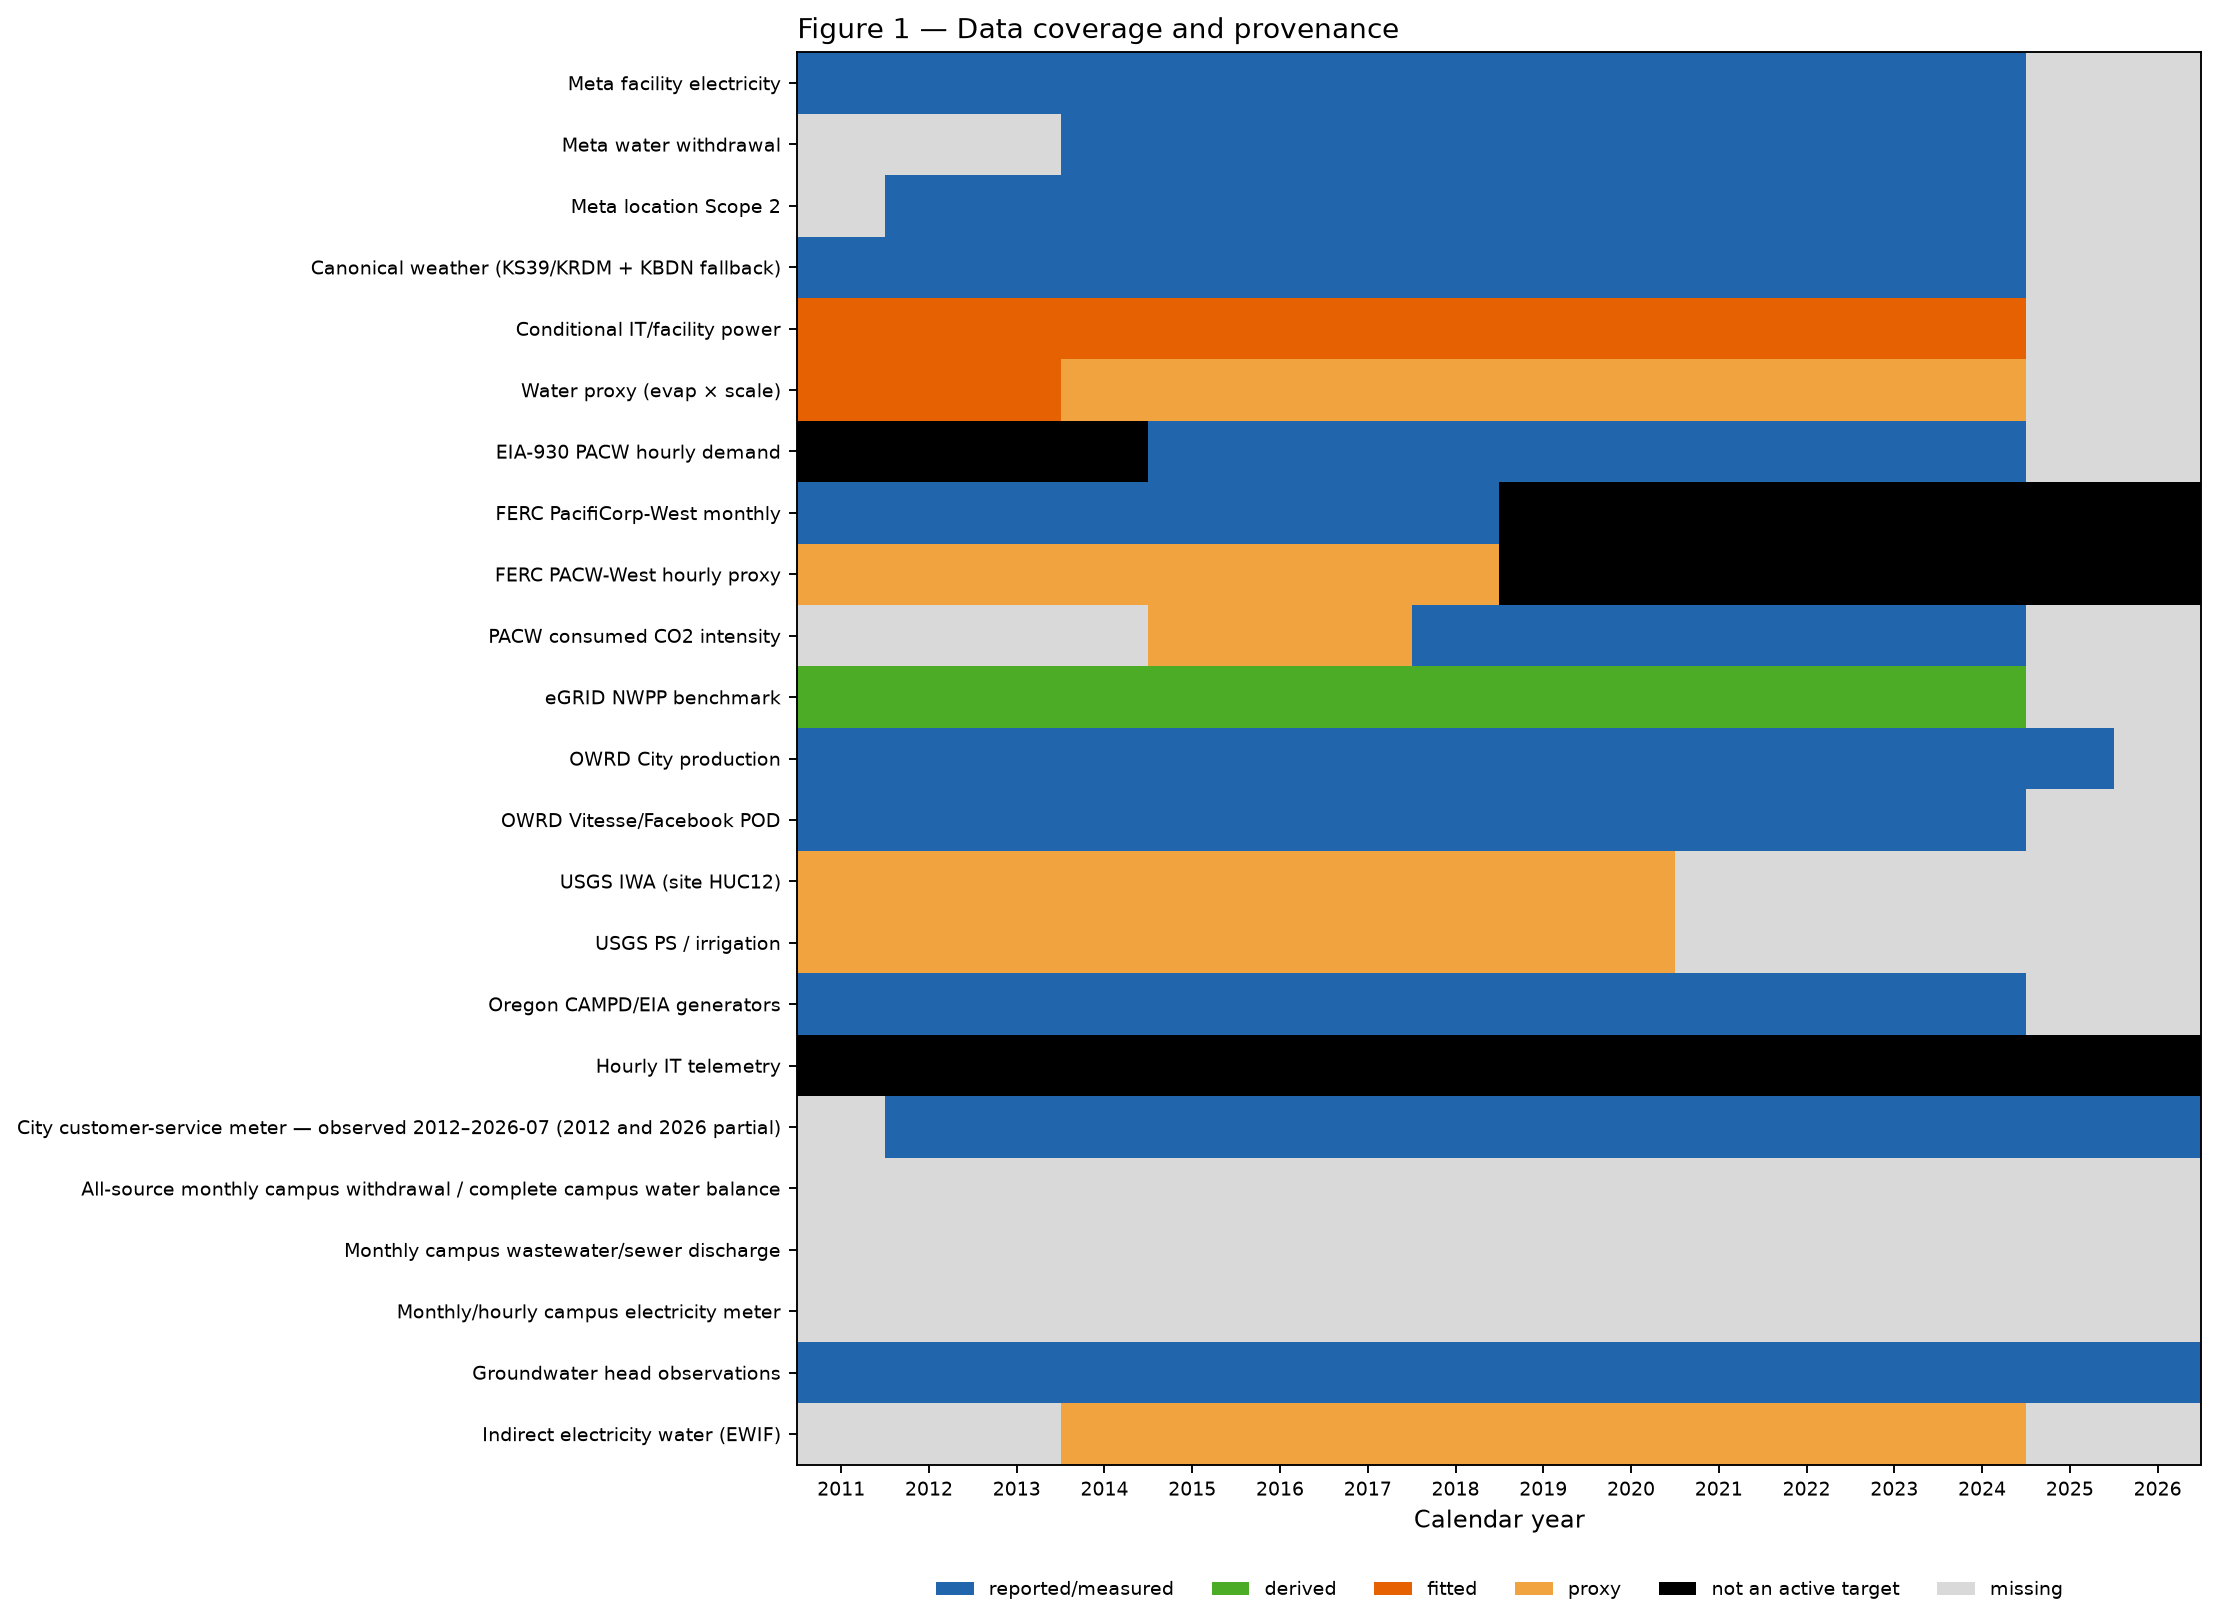
\includegraphics[width=0.86\linewidth]{../../outputs/glossary_refresh_20260903/figures/fig01_data_coverage_provenance.png}
    \caption{\latesttxt{Data coverage and provenance, regenerated from the current Baseline-v2 reporting code. Evidence classes are reported/measured, derived, fitted, proxy, not-an-active-target, or missing over calendar years 2011--2026. Meta annual withdrawal is REPORTED; City WATER-COMM + ADD'L WATER is an OBSERVED customer-service component (2012, 2015, and 2026 partial); all-source monthly Meta/campus withdrawal remains NOT IDENTIFIED. Scope is coverage, not observation density or physical boundary equivalence.}}
    \label{fig:data_coverage}
\end{figure}
% \maybegraphic{fig01_data_coverage_provenanc}
% {Year-by-year coverage status, not a data-density plot. A \Measured{}/\Reported{} cell means a source or measurement exists for that calendar year. For groundwater, that means at least one valid GWIS observation in the year---not monthly completeness or network completeness. \Proxy{} is a model-backed substitute, not a measurement. \NotNecessary{} means not an active acquisition target for the current public-data pipeline, not that the quantity is scientifically useless. Missing remains an active gap.}

% ================================================================
\section{From source to quantity to model}
% ================================================================

The provenance vocabulary used throughout the project is deliberately small:

\begin{center}
\small
\begin{tabularx}{0.96\linewidth}{@{}p{0.16\linewidth}Y@{}}
\toprule
\textbf{Status} & \textbf{Meaning} \\
\midrule
\Reported & Value officially reported by an operator or agency for the stated boundary. \\
\Measured & Direct observational measurement such as weather or groundwater level. \\
\Derived & Computed from observed/validated quantities using an accounting or physical relationship. \\
\Fitted & Estimated from data using a documented statistical or physical model. \\
\Proxy & Substitute for an unavailable target; useful structurally but not claimed as the target measurement. \\
\Scenario & Explicitly assumed or simulated quantity used for sensitivity/counterfactual analysis. \\
\Benchmark & External measured/validated evidence used to test model structure; not transferred numerically to the target site. \\
\NotIdentified & Scientifically relevant quantity/relationship that current evidence does not determine. \\
\NotNecessary & Not an active acquisition target for the present public-data pipeline; not necessarily scientifically unimportant. \\
\bottomrule
\end{tabularx}
\end{center}

\begin{center}
\scriptsize
\begin{tabularx}{\linewidth}{@{}p{0.13\linewidth}p{0.13\linewidth}p{0.14\linewidth}p{0.13\linewidth}Y@{}}
\toprule
\textbf{Layer} & \textbf{Quantity} & \textbf{Source / authority} & \textbf{Status} & \textbf{Model role / current conclusion} \\
\midrule
Workload & \(x_t,u_t\) & none public for Meta & \Scenario & Synthetic workload used only to create plausible operational shapes. \\
IT & \(P^{IT}_t\) & constrained by Meta annual facility MWh & \Fitted / \Scenario & Latent internal state; not directly validated as telemetry. \\
\latesttxt{Modern AI compute} & \latesttxt{\(P^{compute}_{w,N,t}\)} & \latesttxt{NLR/H100 + independent public evidence} & \latesttxt{frozen bounded external evidence} & \latesttxt{Workload/mode/scale conditioning is supported for compute components; full-node AC and facility-IT closure remain uncertain.} \\
Facility & \(E^{fac}_y\) & Meta & \Reported & High-confidence annual target. \\
\newtxt{Facility structure} & \newtxt{\(P^{IT},P^{cool}\)\newline \(P^{fac},PUE\)} & \newtxt{M100 ExaData \cite{m100exadata}} & \newtxt{\Benchmark} & \newtxt{Chronological external validation: explicit weather dependence; PUE derived; cooling dominates M100 non-IT power; dynamic state form remains unidentified.} \\
\oldtxt{Facility archetype intensities} & \oldtxt{\(PUE_k,WUE_k,\)}\newline\oldtxt{\(W^{cond}\)} & \oldtxt{Lei--Masanet \cite{lei2022}} & \oldtxt{external benchmark / in validation} & \oldtxt{First audit: IT-normalized climate--technology intensity model with explicit conditioning-water components; annual envelope/RNG reproduction is the current gate.} \\
\latesttxt{Facility archetype structure} & \latesttxt{\(PUE_k,WUE_k,\)}\newline\latesttxt{\(W^{cond}\)} & \latesttxt{Lei--Masanet \cite{lei2022}} & \latesttxt{\Benchmark; PARTIAL / closed} & \latesttxt{Structure and water-component semantics supported; quantitative adapter promotion blocked by the final reproducibility closure.} \\
\latesttxt{Facility overhead regime structure} & \latesttxt{\(P^{overhead},\)}\newline\latesttxt{\(A^{arch},S^{op}\)} & \latesttxt{NLR/ESIF \cite{esifdata}} & \latesttxt{\Benchmark; PARTIAL / closed} & \latesttxt{Stationary IT+weather total-aux hypothesis fails; architecture/configuration and operating state must be allowed when spanning facility epochs.} \\
\oldtxt{Independent facility response} & \oldtxt{\(P^{IT}\rightarrow P^{accessory}\)} & \oldtxt{Frontier \cite{frontier2024}} & \oldtxt{external benchmark / QC pending} & \oldtxt{First chronological result: affine IT-load model improves accessory-power MAE in all 9 folds; gap-safe coverage/energy correction is running.} \\
\latesttxt{Independent facility response} & \latesttxt{\(P^{IT}\rightarrow P^{accessory}\)} & \latesttxt{Frontier \cite{frontier2024}} & \latesttxt{\Benchmark; closed} & \latesttxt{Corrected gap-safe audit leaves the all-9-fold load-dependence conclusion unchanged; no site-water/WUE inference.} \\
Weather & \(T,T_d,T_{wb},p\) & NOAA & \Measured / \Derived & Strong cooling input layer. \\
Cooling & \(P^{cool}_t,Q^{cool}_t\) & gray-box & \Derived & Mechanism/scenario quantity. \\
Campus water & \(W^{Meta}_y\) & Meta & \Reported & High-confidence annual withdrawal target for 2014--2024; withdrawal is not consumption. \\
\latesttxt{City customer-service water} & \latesttxt{\(W^{City,service}_m\)} & \latesttxt{City of Prineville utility records} & \latesttxt{\Reported} & \latesttxt{Observed Facebook Data Center WATER-COMM + ADD'L WATER monthly service component; not total campus withdrawal and not a source allocation.} \\
\latesttxt{All-source monthly campus withdrawal} & \latesttxt{\(W^{Meta,total}_m\)} & \latesttxt{no closed source/accounting bridge} & \latesttxt{\NotIdentified} & \latesttxt{City service is one observed component; bulk/SWR/WELL/direct-POD/reuse/return/storage and scope relations do not identify the campus total.} \\
Evaporation & \(W^{evap}_t\) & gray-box & \Derived & Physical cooling mechanism, not total campus withdrawal. \\
Municipal/direct pumping & \(Q_t\) & OWRD & \Reported & Water-system / groundwater forcing at explicit reporting boundaries. \\
Regional water context & HUC12 use / availability & USGS & \Proxy & Regional context only; not a campus or aquifer measurement. \\
Grid demand & \(D^{PACW}_t\) & EIA + FERC & \Measured / \Proxy & EIA later; FERC historical bridge earlier. \\
Carbon & \(CI_t\) & EIA / EPA eGRID & \Derived / \Proxy & Regional average/accounting context. \\
Plant impacts & \(G_{g,t},CO_{2,g,t}\)\newline \(W_{g,t}\) & EIA / EPA & \Reported / \Derived & Generator-level context; no Meta-specific serving attribution. \\
Groundwater level & \(BLS_{i,t}\) / reported AMSL & OWRD GWIS & \Measured & QC-qualified individual-well observations; not a spatial/network head field. \\
Within-well relative head & \(\tilde h_{i,t}\) & derived from GWIS & \Derived & \(\tilde h_{i,t}=-(BLS_{i,t}-\overline{BLS}_i)\); physically signed target for the planned empirical benchmark. \\
Facility chronology & technology/events & Crook County & \Reported & Documentary evidence of expansion/cooling regime changes. \\
Groundwater response / state & \((\beta,A,B_R,B_Q)\) & not yet estimated & \NotIdentified & Empirical pumping response is the immediate benchmark; a reduced spatial/network state remains future work. \\
Decision variables & workload / siting / source choice & future & \Scenario & Long-run optimization layer after response models are validated. \\
\bottomrule
\end{tabularx}
\par\smallskip{\small\itshape Master source--quantity--model map. Appendix~\ref{app:quantities} provides the complete machine-traceable version.\par}\end{center}

% ================================================================
\section{The model: general structure and current Prineville approximation}
% ================================================================

The literature suggests a coherent coupled spine. The Prineville implementation intentionally uses the simplest version supported by available public data.

\subsection[Workload to IT power]{Workload \(\rightarrow\) IT power}

A general operational model would begin with
\[
E^{IT}_{t}
=
\mathcal P(x_t,u_t,\text{hardware},\text{workload})\Delta t.
\]

\textbf{Prineville:} workload and server telemetry are not public. \(P^{IT}_t\) is therefore latent/scenario-based, not measured.

\newtxt{For the generic model, keep server/node power and the facility IT meter as distinct boundaries:
\[
P^{IT,fac}_t
=
\mathcal A_h\!\left(\{P^{node}_{j,t}\}_{j=1}^{N_t};\theta^{IT}_h\right).
\]
M100 validates the need for this mapping: summed qualified node power strongly tracks the canonical facility IT meter but covers only roughly \(74.5\)--\(80.9\%\) of \(Tot\_ict\), so node power must not be equated mechanically with facility IT power.}

\oldtxt{The next compute-side experiment is already specified under \path{other_sources/it_power}: NLR, the 2026 H100/B200 dataset, and MLPerf Power provide complementary device/node/system boundaries. This is an experimental design only; no generic workload--power map is yet validated.}

\latesttxt{The modern AI IT-power layer under \path{other_sources/it_power} now has machine disposition \path{FROZEN_BOUNDED_WITH_EXPLICIT_NODE_UNCERTAINTY}. Controlled CPU/H100 evidence supports workload-, mode-, scale-, and temporal-profile conditioning for compute-component power. It does not close full-node AC, other-node power, the production workload mix, or the node/system-to-facility-IT boundary.}

\subsection[IT power to facility electricity and cooling]{IT power \(\rightarrow\) facility electricity and cooling}

\oldtxt{The generic reading of the current scaffold is \(P^{fac}_t=P^{IT}_t+P^{fan}_t+P^{other}_t+P^{cool,aux}_t\).}

\newtxt{The externally validated generic accounting boundary should instead be written as}
\[
{\color{green!45!black}
P^{fac}_t
=
P^{IT}_t
+
P^{cool}_t
+
P^{aux}_t,
}
\]
\[
{\color{green!45!black}
P^{cool}_t
=
f_k\!\left(P^{IT}_t,\mathbf w_t,s_t;\theta_k\right),
\qquad
PUE_t=\frac{P^{fac}_t}{P^{IT}_t}.
}
\]
\newtxt{Here \(k\) is a facility/cooling archetype, \(\mathbf w_t\) is the relevant weather vector, and \(s_t\) is an optional latent/operating state. M100 strongly supports explicit weather dependence and derived \(PUE\); it does \emph{not} identify universal coefficients, a universal weather variable, or a validated generic state equation.}

\oldtxt{For strategic/planning models, the minimum currently supported form is \(P^{cool}_t=f_k(P^{IT}_t,\mathbf w_t;\theta_k)\).}

\oldtxt{The first Lei--Masanet audit supports a simpler \emph{planning intensity backbone}:}

\latesttxt{Lei--Masanet supports the following \emph{model class} as a climate--technology intensity abstraction, but its final reproducibility closure blocks promotion of the public implementation as a quantitative project adapter:}
\[
{\color{green!45!black}
P^{fac}_t
=
P^{IT}_t\,PUE_k(\mathbf w_t,\theta_k),
\qquad
P^{nonIT}_t
=
P^{IT}_t\bigl[PUE_k(\mathbf w_t,\theta_k)-1\bigr].
}
\]
\newtxt{This uses climate and cooling-technology archetype \(k\) to determine facility intensity; it does not claim that Lei--Masanet identifies nonlinear IT part-load behavior. The more general decomposition \(P^{fac}=P^{IT}+P^{cool}+P^{aux}\) remains the accounting architecture, and a dynamic \(f_k(P^{IT},\mathbf w,s)\) should be introduced only if later operational evidence makes it decision-relevant.}

\latesttxt{ESIF adds a separate caution on stationarity. When a model spans infrastructure/configuration epochs, the minimum supported predictive structure may require explicit architecture and operating-state variables:}
\[
{\color{purple!85!black}
P^{overhead}_t
=
f_k\!\left(P^{IT}_t,\mathbf w_t,A^{arch}_t,S^{op}_t;\theta_k\right),
\qquad
P^{fac}_t=P^{IT}_t+P^{overhead}_t.
}
\]
\latesttxt{Here \(A^{arch}_t\) denotes facility/hardware/configuration epoch and \(S^{op}_t\) an operating/control state. This is a structural allowance, not an identified universal state equation and not permission to transfer ESIF coefficients.}

\newtxt{With variable IT load, annual PUE must be energy-weighted:}
\[
{\color{green!45!black}
PUE_y
=
\frac{\sum_{t\in y}P^{fac}_t\Delta t}
     {\sum_{t\in y}P^{IT}_t\Delta t},
}
\]
\newtxt{not an unweighted arithmetic mean of hourly PUE. The two coincide in the upstream Lei--Masanet reproduction only because it normalizes hourly \(P^{IT}=1\). PUE accounting should follow ISO/IEC 30134-2 \cite{isoPUE}; PUE remains a derived KPI, not an independently sampled primitive.}

\textbf{Prineville implementation.} The annual IT scale is chosen so that
\[
\sum_{t\in y}P^{fac}_t\Delta t=E^{Meta}_y.
\]

\textbf{Interpretation:} this is an annual-closed reconstruction. The exact annual match is an accounting/calibration closure, \emph{not} electricity forecast accuracy.

\subsection[Cooling/facility to conditioning and source water]{\oldtxt{Cooling \(\rightarrow\) direct water} \newtxt{Cooling/facility \(\rightarrow\) conditioning water \(\rightarrow\) source water}}

\oldtxt{The earlier generic water block mapped cooling directly to separate withdrawal and consumption response functions.}

\newtxt{The first Lei--Masanet audit identifies an intermediate facility-side quantity more directly: modeled onsite \emph{conditioning-water use}. For interval \(t\),}
\[
{\color{green!45!black}
W^{cond}_t
=
E^{IT}_t\,WUE_k(\mathbf w_t,\theta_k),
}
\]
\newtxt{where the upstream model's water total includes cooling-tower evaporation, windage/drift, draw-off/blowdown, adiabatic/direct evaporative cooling, and humidification. This is an IT-normalized climate--technology intensity model; it does not separately identify source withdrawal, total consumption, return/discharge, or source shares.}

\newtxt{Therefore the coupled project must retain an explicit second bridge:}
\[
{\color{green!45!black}
W^{cond}_t+W^{other}_t
\longrightarrow
\{W^{with}_t,W^{cons}_t,W^{return}_t\}
\longrightarrow
\{W^{municipal}_t,W^{direct\,gw}_t,W^{reuse}_t,\ldots\}
\longrightarrow q^{gw}_t.
}
\]
\newtxt{In particular, \(WUE_k E^{IT}\neq\) groundwater pumping. M100 independently reinforces this boundary because its liquid-loop flow is circulation, not site water use.}

\newtxt{With variable IT load, annual conditioning-water intensity must also be energy-weighted:}
\[
{\color{green!45!black}
WUE_y
=
\frac{\sum_{t\in y}W^{cond}_t}
     {\sum_{t\in y}E^{IT}_t}.
}
\]
\newtxt{The current project should keep this modeled conditioning-water intensity distinct from Meta withdrawal intensity and from any future source-resolved withdrawal/consumption accounting.}
\oldtxt{Facility-water gate now running: annual Lei--Masanet envelope/RNG reproduction must pass before the adapter is used. The 2023--2024 Meta water holdout remains untouched. Source withdrawal/return/reuse still require separate evidence.}

\latesttxt{\textbf{Lei--Masanet closure.} Final disposition is PARTIAL and quantitative adapter promotion is NO/blocked. The climate--technology intensity structure and conditioning-water components remain useful evidence, but exact quantitative envelopes are not treated as a validated generic project adapter. The frozen Meta 2023--2024 water holdout was not read during the closure.}

The current Prineville gray-box estimates a raw evaporative requirement from weather, airflow, heat load, and simplifying cooling assumptions. A parsimonious annual model then fits
\[
\widehat W_y=s\,W^{evap}_y
\]
or related energy/evaporation regressions to annual Meta withdrawal.

\textbf{Interpretation:} \(W^{evap}\) is a physical mechanism, not total campus withdrawal. The fitted scale absorbs unobserved non-cooling use, blowdown/reuse differences, architecture changes, and model error.

\latesttxt{\textbf{New Prineville observation.} The City public-records integration now provides a directly observed monthly customer-service quantity}
\[
{\color{purple!85!black}
W^{City,service}_m
=
\sum_{r\in\mathcal R_{service}}W^{City}_{r,m},
\qquad
\mathcal R_{service}=\{\text{WATER-COMM},\ \text{ADD'L WATER}\},
}
\]
\latesttxt{with source units of 100 ft\(^3\) per reported unit (748 US gal). This is a downstream municipal-service boundary. It is not \(W^{Meta,total}_m\), not consumption, not municipal production, and not groundwater pumping. Bulk/hydrant, SWR METER, WELL METER FOR SEW, Trailer City, and Warehouse remain separate until their accounting relationships are identified.}

\subsection[Facility electricity to regional grid, carbon, and generator water]{Facility electricity \(\rightarrow\) regional grid, carbon, and generator water}

Attributionally,
\[
\widehat{CO}_{2,t}=CI_tE^{grid}_t,
\qquad
\widehat W^{ind}_t=EWIF_tE^{grid}_t.
\]

Modern regional demand comes from EIA-930. Historical PACW-West hourly demand is reconstructed using FERC Form 714 monthly West totals plus East+West hourly shape, then validated against EIA-930 in overlap years.

\textbf{Interpretation:} these are regional accounting/context layers. They do not identify Meta's exact serving generators or marginal grid response.

\subsection[Water-source pumping to groundwater state]{Water-source pumping \(\rightarrow\) groundwater state}

\oldtxt{Earlier notation mapped groundwater forcing from a single \(W^{dir,with}\) quantity.}

\newtxt{The eventual coupled model should instead use the source-resolved groundwater share of facility withdrawal:}
\[
{\color{green!45!black}
q^{dc}_{n,\tau}
=
\theta^{gw}_{n,\tau}W^{with}_{\tau},
}
\]
\newtxt{where \(\theta^{gw}_{n,\tau}\) is an explicitly identified groundwater/source allocation, not an assumed conversion from WUE or conditioning water. This forcing then enters a reduced groundwater state model such as}
\[
h_{\tau+1}
=
Ah_\tau+B_RR_\tau-B_Qq_\tau+\varepsilon_\tau.
\]

\textbf{Prineville today:} source shares and physical aquifer parameters are not identified. What we observe directly are well-specific GWIS BLS/AMSL measurements. For the first benchmark we derive a within-well, physically signed relative head anomaly, \(\tilde h_{i,t}=-(BLS_{i,t}-\overline{BLS}_i)\). This is enough to test a simple empirical pumping-response relationship, but it is not a common-datum spatial groundwater state and does not identify \(A,B_R,B_Q\).

\subsection{Simulation and future decisions}

The stochastic workload module generates plausible workload/utilization shapes,
\[
\text{synthetic arrivals}
\rightarrow
u_t
\rightarrow
P^{IT}_t
\rightarrow
\text{energy / cooling / water / carbon scenarios}.
\]

Simulation is therefore an \textbf{experiment engine}: it can explore interactions under explicit assumptions, but it cannot recover missing historical telemetry or establish causal groundwater impacts.

\newtxt{\textbf{Model-fidelity principle.} The eventual planning model should compare a fixed-coefficient baseline, a validated climate--technology archetype model, and only if needed a higher-fidelity dynamic model by \emph{decision relevance}---regret, changed site/cooling/source choices, capacity or groundwater violations, and environmental/equity outcomes---not only by predictive fit.}

% ================================================================
\section{How the literature maps to the model}
% ================================================================

The project is deliberately not trying to implement every ``state-of-the-art'' model at once. The relevant question is which literature structure is justified by the data at each layer.

\begin{center}
\scriptsize
\begin{tabularx}{\linewidth}{@{}p{0.17\linewidth}p{0.20\linewidth}p{0.21\linewidth}Y@{}}
\toprule
\textbf{Literature family} & \textbf{What we inherit} & \textbf{Current Prineville approximation} & \textbf{What would justify the next upgrade?} \\
\midrule
\newtxt{Measured facility telemetry: M100 ExaData \cite{m100exadata}} & \newtxt{Measured IT/facility/cooling/weather relationships and accounting boundaries} & \newtxt{External structural benchmark; no coefficient transfer to Prineville} & \newtxt{Completed v3 closure; use findings as model constraints, then stop M100 fitting.} \\
\newtxt{Thermal dynamics on M100 \cite{m100dynamic}} & \newtxt{Same-data literature triangulation that dynamic cooling states can matter} & \newtxt{Interpretive support only; not independent validation} & \newtxt{Use independent facilities/models before adopting a dynamic state equation.} \\
National/accounting: LBNL; Siddik et al.\ \cite{lbnl2024,siddik2021} & Explicit system boundaries, aggregate envelopes, spatial environmental accounting & Site-specific reported annual quantities + regional context & Use mainly as external order-of-magnitude / boundary checks. \\
Facility PUE/WUE: Lei \& Masanet\ \cite{lei2020,lei2022} & Climate- and technology-dependent coupled energy/water physics & \oldtxt{Next generic archetype layer: cooling power, withdrawal, and consumption as climate/technology-dependent outputs} \newtxt{First audit complete: IT-normalized PUE/WUE intensity backbone with explicit conditioning-water components} & \oldtxt{Annual 50-LHS\(\times\)8760 reproduction, hidden-RNG gate, adapter tests, and Prineville-2022-weather translation are running; no Meta water holdout is read.} \latesttxt{Final closure PARTIAL; adapter promotion blocked. Retain structural/intensity evidence and water-component definitions, not a quantitative generic adapter.} \\
\newtxt{Independent thermal/power benchmark: Frontier \cite{frontier2024}} & \newtxt{Measured compute/accessory power and coolant telemetry on a different liquid-cooled facility} & \oldtxt{Not yet integrated} \newtxt{First chronological F0/F1/F2 test complete: IT-load term improves accessory-power MAE in all 9 folds} & \oldtxt{Gap-safe expected-time-grid/energy QC correction is running; thermal-field reproduction is not independent conservation validation.} \latesttxt{Corrected gap-safe audit is CLOSED; coverage is about 93.4\% and the F1-vs-F0 qualitative conclusion is unchanged. Thermal reconstruction remains formula reproduction, not independent conservation.} \\
\latesttxt{Measured facility overhead: NLR/ESIF \cite{esifdata}} & \latesttxt{Measured IT, component overhead, PUE, and weather across a long facility history} & \latesttxt{Electrical overhead layer closes PARTIAL; stationary IT+weather total-aux hypothesis FAILS across the 2024 regime change} & \latesttxt{Use \(f(P^{IT},\mathbf w,A^{arch},S^{op})\) as the minimum cross-epoch structural allowance; do not transfer coefficients or site PUE values.} \\
\oldtxt{Modern AI IT-power evidence: NLR / H100--B200 / MLPerf} & \oldtxt{Device, node, and system power at complementary boundaries} & \oldtxt{Source audit and smallest nested experiment are predeclared under \path{other_sources/it_power}} & \oldtxt{No generic workload\(\rightarrow P^{IT}\) map is yet validated; preserve device/node/system/facility boundaries.} \\
\latesttxt{Modern AI IT-power evidence: NLR / H100 + independent public evidence} & \latesttxt{Workload-, mode-, scale-, and temporal-profile-conditioned compute-component power} & \latesttxt{Frozen bounded external layer with explicit node uncertainty} & \latesttxt{Use workload-specific compute scenarios; full-node AC, other-node power, production mix, and the facility-IT bridge remain unresolved.} \\
Water footprint: Li et al.; Gupta et al.; Han et al.\ \cite{li2023,gupta2024,han2026} & Direct vs indirect water; temporal water signals; peak public-water capacity & \oldtxt{Annual direct water + partial regional generator-water diagnostics} \latesttxt{Annual Meta withdrawal + observed monthly City-service component + partial regional generator-water diagnostics} & \oldtxt{Monthly campus water, source shares, withdrawal/consumption/discharge, peak delivery.} \latesttxt{All-source monthly campus withdrawal, source shares, withdrawal/consumption/return, and peak delivery remain unresolved.} \\
Operational scheduling: WACE; Google; WaterWise; TAPAS\ \cite{wace,googlecarbon,waterwise,tapas} & Workload conservation, spatial/temporal flexibility, carbon/water/thermal constraints & Stochastic scenarios only; no actual workload optimization yet & Real workload flexibility/capacity, validated environmental response signals, prices/costs. \\
Siting/planning: PSCC project\ \cite{projectpscc} & Cost--carbon--water--equity planning backbone & Long-run target, not current implementation & Credible source-specific water and groundwater response functions. \\
Groundwater: MODFLOW / hydro-economic models\ \cite{modflow,harou2009} & Pumping/recharge \(\rightarrow\) head/storage dynamics; multi-sector allocation & First empirical well-level benchmark only & Recharge/background forcing and sufficient hydrogeologic/response information for reduced-order or physical calibration. \\
\bottomrule
\end{tabularx}
\par\smallskip{\small\itshape Literature-to-model map: what is inherited now, what is simplified, and what evidence would justify more complexity.\par}\end{center}

% ================================================================
\section{External facility-model validation: M100 ExaData}
% ================================================================

\newtxt{M100 is used only as an \Benchmark{} for the missing internal facility layer. The canonical record is the v3 closure under
\path{other_sources/m100/results/suitability_2021_v3_closure/}; Apr--Dec 2021 provide nine qualified full-facility months and eight expanding chronological test folds (May--Dec). The primary target is \(P^{nonIT}=Tot-Tot\_ict\); a validated cooling-power aggregate is a secondary target.}

\begin{center}
\scriptsize
\begin{tabularx}{\linewidth}{@{}p{0.25\linewidth}p{0.37\linewidth}Y@{}}
\toprule
\textbf{Claim tested} & \textbf{M100 experiment / evidence} & \textbf{Model consequence} \\
\midrule
\newtxt{Facility accounting boundary} &
\newtxt{Canonical \(Tot\) and \(Tot\_ict\) pass strong internal checks; validated cooling components explain about \(95.5\)--\(98.2\%\) of M100 non-IT energy.} &
\newtxt{Use \(P^{fac}=P^{IT}+P^{cool}+P^{aux}\); do not transfer the M100 cooling share.} \\

\newtxt{Weather dependence} &
\newtxt{Adding weather to affine IT load improves held-out MAE in \(8/8\) expanding folds (about \(42\%\) mean improvement) and in \(7/9\) fixed within-month tests. Dry-bulb and wet-bulb variants both carry signal.} &
\newtxt{Weather must be explicit; do not hard-code a universal weather variable.} \\

\newtxt{IT--weather interaction} &
\newtxt{The predeclared \(P^{IT}\!\times T_{wb}\) interaction adds \(\ge5\%\) MAE improvement in \(0/8\) folds.} &
\newtxt{Do not require this interaction in the minimum generic model.} \\

\newtxt{Observed free-cooling state} &
\newtxt{A regime/state enrichment is stably useful in only \(2/8\) folds and worsens most later folds.} &
\newtxt{Do not expose M100 \texttt{Free\_Cooling\_Status} as a required generic input.} \\

\newtxt{Temporal state/dynamics} &
\newtxt{Static residuals have strong 1-h persistence; a one-step lag oracle helps strongly, but the tested recursive D1 simulator is worse than the static weather model in \(7/8\) folds.} &
\newtxt{Allow a future dynamic state for operational simulation, but its form is not identified by M100.} \\

\newtxt{Node \(\rightarrow\) facility IT boundary} &
\newtxt{Summed qualified node power tracks \(Tot\_ict\) but covers only about \(74.5\)--\(80.9\%\) of that boundary.} &
\newtxt{Require a server/node-to-facility-IT aggregation map; do not equate GPU/node watts with facility IT watts.} \\

\newtxt{Thermal transport} &
\newtxt{\(P^{IT}\) vs.\ \(flow\times\Delta T\) is positively associated (Pearson roughly \(0.45\)--\(0.89\)) on qualified periods; Sep--Oct twin-panel behavior is unresolved.} &
\newtxt{Qualitative thermal sanity only; no M100 thermal-kW closure or water-consumption claim.} \\

\newtxt{Water use} &
\newtxt{No independently verified makeup/withdrawal/consumption meter was found; circulating flow is not site water use.} &
\newtxt{M100 cannot identify WUE, withdrawal, or consumptive-water parameters.} \\
\bottomrule
\end{tabularx}
\end{center}

\newtxt{\textbf{Bottom line.} M100 falsifies a weather-independent fixed-efficiency facility model across changing conditions and supports an archetype-based response \(P^{cool}=f_k(P^{IT},\mathbf w,\text{optional state})\). It validates structure, not generic coefficients.}

\newtxt{\textbf{QC limits retained in the record.} The processed tables support strong energy-integral/gap robustness but not a reconstructed \(\ge90\%\) raw source-sample coverage test. October's reported-PUE channel is anomalous while canonical \(Tot/Tot\_ict\) remains usable. The 2026 dynamic-model code was executable but did not numerically reproduce its bundled sample exactly, so it is treated only as same-data literature triangulation.}
\todo[inline]{After the M100 reporting cleanup is merged, record the final git commit/hash here for immutable provenance.}

% ================================================================
\section[External facility evidence beyond M100]{\oldtxt{Facility energy--water archetype validation: Lei--Masanet + Frontier}\ \latesttxt{External facility evidence beyond M100: Lei--Masanet, Frontier, ESIF, and transferability}}
% ================================================================

\oldtxt{The next external-validation layer asks whether the planning model can replace fixed PUE/water coefficients with climate--technology intensities without pretending to recover a specific private facility. The first Lei--Masanet audit is complete; a bounded publication-scale annual reproduction is currently running. Frontier supplies a separate measured power/thermal check.}

\latesttxt{This layer is now mostly a \emph{claim-restriction} exercise rather than an open-ended model search. M100 is frozen; Frontier's corrected QC is closed; ESIF's electrical overhead experiment is closed PARTIAL; Lei--Masanet's final reproducibility closure is PARTIAL with adapter promotion blocked. Together they support a reduced structural family, but not a universal coefficient set.}

\newtxt{PUE and WUE should be generated jointly from the same archetype, weather, and facility-parameter draw rather than sampled independently. LBNL is used only for qualitative technology/envelope triangulation because it shares modeling/authorship lineage with Lei--Masanet; it is not counted as independent validation.}

{\color{purple!85!black}
\begingroup
\scriptsize
\setlength{\tabcolsep}{3pt}
\setlength{\emergencystretch}{3em}
\raggedright
\sloppy
\begin{longtable}{@{}p{0.120\linewidth}p{0.150\linewidth}p{0.230\linewidth}p{0.230\linewidth}p{0.190\linewidth}@{}}
\caption{Final frozen external-validation synthesis. These streams constrain model structure at their stated boundaries; none supplies a calibrated Prineville facility/water model.}\\
\toprule
\textbf{Evidence stream} & \textbf{Final status} & \textbf{Strongest supported result} & \textbf{Not identified / prohibited inference} & \textbf{Model consequence} \\
\midrule
\endfirsthead
\toprule
\textbf{Evidence stream} & \textbf{Final status} & \textbf{Strongest supported result} & \textbf{Not identified / prohibited inference} & \textbf{Model consequence} \\
\midrule
\endhead
\midrule
\multicolumn{5}{r}{\emph{Continued on next page}}\\
\endfoot
\bottomrule
\endlastfoot
M100 & CLOSED / FROZEN; limitations & Measured accounting and weather structure; node power strongly bridges to, but is not equal to, facility IT. & No generic coefficient/PUE/cooling-fraction/water transfer; node/system is not facility IT. & Retain explicit IT + weather facility structure and boundary separation. \\
Frontier & CLOSED & Independent 9-fold evidence that IT load improves accessory-power prediction; corrected time-grid coverage 93.4\%. & No WUE, withdrawal, site-water, or transferable thermal coefficient claim. & Retain IT-load-dependent accessory-power structure; thermal formula is an accounting reproduction. \\
Lei--Masanet & PARTIAL / CLOSED; adapter blocked & Climate-by-technology intensity and onsite conditioning-water component structure are useful. & No quantitative adapter promotion, nonlinear IT-load twin, source/groundwater inference, or Meta calibration. & Use only bounded qualitative/archetype scenarios; preserve P\_IT=1 intensity semantics. \\
NLR/ESIF facility overhead & PARTIAL / CLOSED & Stationary IT+weather total-overhead mapping fails across the persistent 2024 HVAC/configuration regime shift. & No coefficient transfer or claim that one cross-epoch HVAC law is validated. & Include architecture/configuration and operating state; validate components and epochs. \\
Forest City v3 & Qualitative PARTIAL; quantitative NOT VALIDATED & Same-window climate/controller replay supports mechanism-specific transportability and station-robust zero summer DX. & Effective facility Delta-T, airflow, cooling-only water, and numerical transfer remain unidentified; model not calibrated. & Transfer qualitative mechanisms only; engineering/utility records bind further progress. \\
Modern AI IT-power layer & FROZEN / BOUNDED; node uncertainty & Controlled CPU/H100 compute-component energy is workload/mode/scale conditioned; independent H100 sanity check passes. & Full-node AC and same-system component-to-node bridge are unsupported; production workload mix and facility IT boundary remain incomplete. & Use bounded workload-specific compute scenarios plus explicit uncertainty for other-node, network, storage, and service power. \\
\end{longtable}
\endgroup

}

{\small
\oldtxt{\textbf{Current annual validation gate.}} \oldtxt{The paper/code case crosswalk passed 12 focused tests.}\\
\oldtxt{Six case\(\times\)climate cells were then locked} \oldtxt{before inspecting reproduction errors}\\
\oldtxt{and span wet/waterside, air-cooled, DX, economizer,} \oldtxt{hot/humid, and cold regimes.}\\
\oldtxt{Each is evaluated using the paper-style} \oldtxt{\(50\) LHS facility samples \(\times 8760\) TMY hours.}\\
\oldtxt{Hidden upstream RNG is tested separately} \oldtxt{against facility-parameter uncertainty.}\\
\oldtxt{Only if this gate passes do adapter tests} \oldtxt{and a Prineville-2022-weather translation proceed;}\\
\oldtxt{the frozen Meta 2023--2024 water holdout is never read.}\par}

\latesttxt{\textbf{Closed Lei--Masanet verdict.} The final reproducibility closure is PARTIAL and adapter promotion is NO/blocked. The physical/accounting/climate--technology structure remains useful, but exact quantitative envelopes are only partially compatible; no seed search, range tuning, weather substitution, or upstream-physics edit was used to rescue the result. The protected Meta 2023--2024 water holdout remained unread.}

{\small
\oldtxt{Replace this running-status paragraph with the canonical}\\
\oldtxt{FOLLOWUP\_V1\_STATUS.json / FOLLOWUP\_V1\_SUMMARY.md}\\
\oldtxt{result once the DAG completes.}\\
\oldtxt{If the annual/RNG gate fails,} \oldtxt{keep Lei--Masanet as qualitative archetype evidence}\\
\oldtxt{rather than a project adapter.}\par}

{\color{purple!85!black}
\textbf{Forest City v3 transferability check.} The frozen cross-site experiment ends with:
\begin{itemize}
\item \path{QUANTITATIVE_PHYSICS_TRANSFER=NOT_VALIDATED};
\item \path{FACILITY_EFFECTIVE_DELTA_T=UNIDENTIFIED};
\item \oldtxt{\path{COOLING_WATER_MAGNITUDE=UNIDENTIFIED};}
\item \latesttxt{\path{FRC1_COOLING_ONLY_WATER_MAGNITUDE=UNIDENTIFIED};}
\item \path{MODEL_CALIBRATED=NO}.
\end{itemize}
It provides strong same-window climate evidence and useful weather\(\times\)controller decomposition, but only PARTIAL qualitative physics transfer. This reinforces the rule: transfer structure, not numerical coefficients.
}

% ================================================================
\section{What we have learned so far}
% ================================================================

\subsection*{1. The case is now empirically rich enough to ground the research question}

Meta Prineville grew from a comparatively small early campus to a facility using electricity at the TWh/year scale. Reported campus electricity covers 2011--2024 (71{,}000~MWh to 1.73~TWh). Water withdrawal is reported from 2014. Location-based Scope 2 is reported from 2012; 2011 is not separately disclosed. Annual campus electricity, water withdrawal, and location-based Scope 2 evolve differently, which already shows that one single ``size'' proxy cannot explain every externality.


\begin{figure}
    \centering
    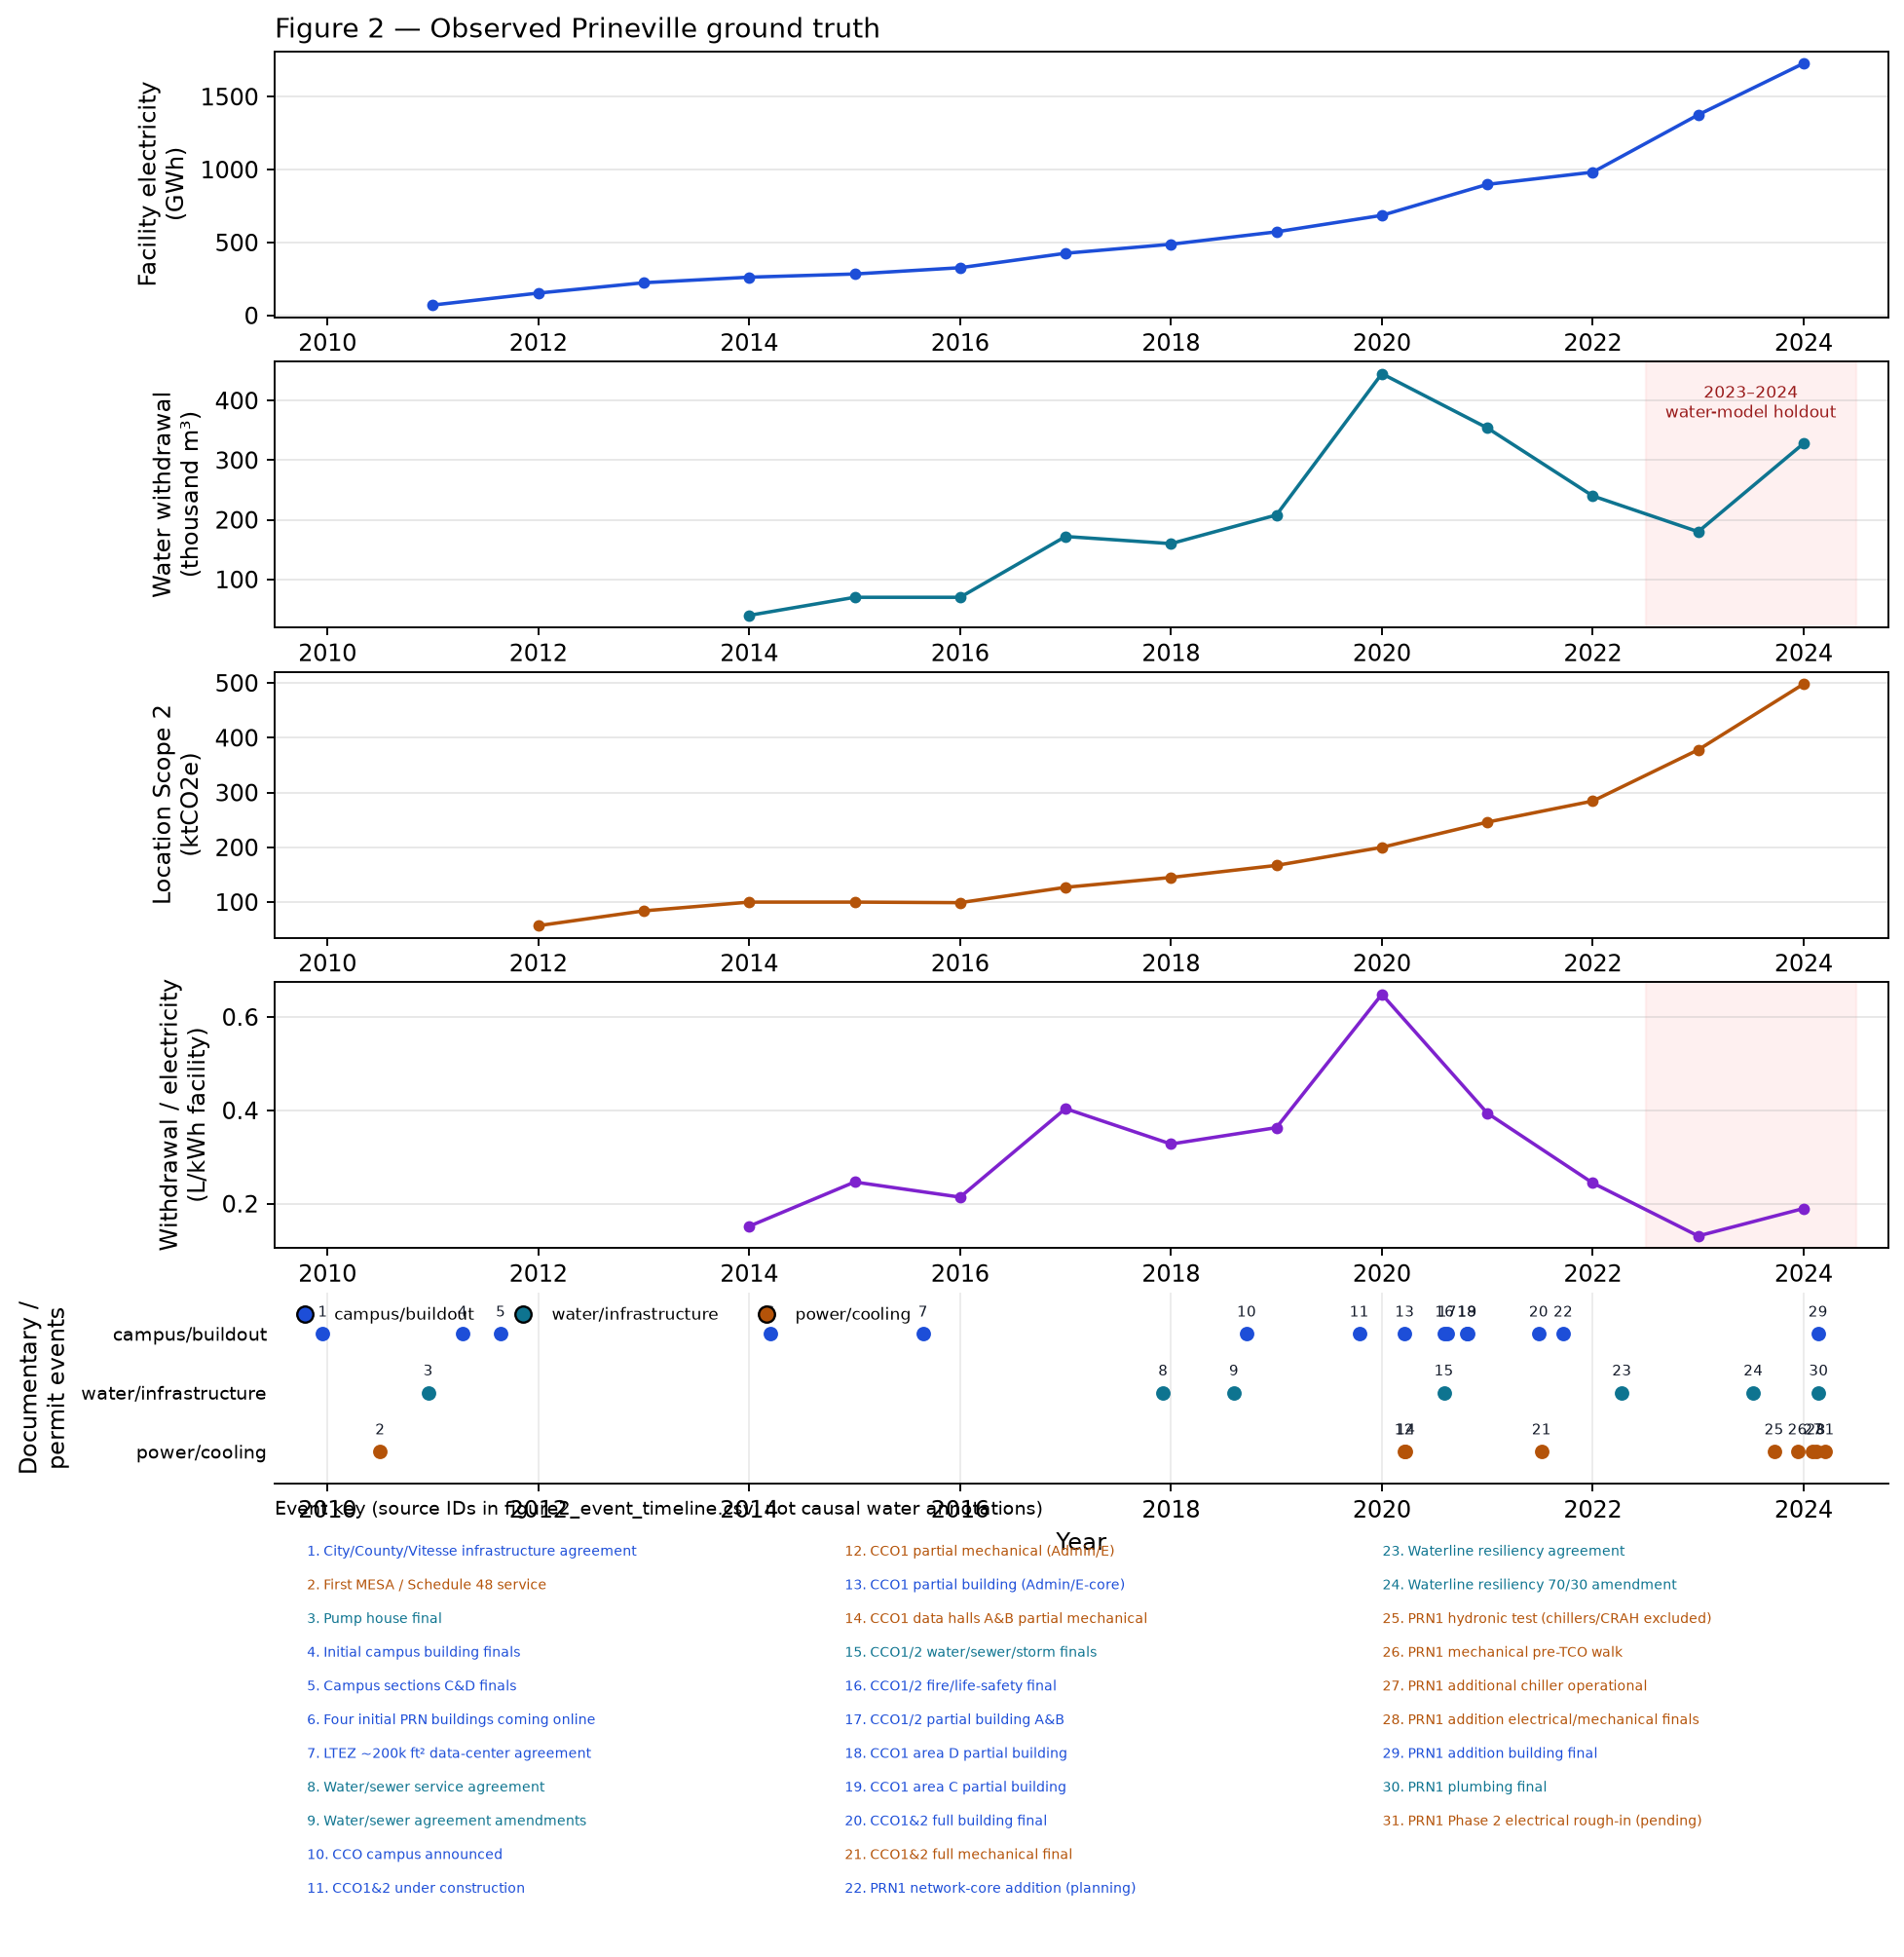
\includegraphics[width=0.8\linewidth]{../../Meta_Prineville_Oregon_v3/outputs/pipeline_report/figures/fig02_observed_ground_truth.png}
    \caption{Observed annual Meta Prineville ground truth and intensity evolution. This is the empirical anchor for the case study. \latesttxt{Evidence class: REPORTED operator disclosures; campus annual scope; electricity (n=14) (2011--2024, GWh), water withdrawal (n=11) (2014--2024, thousand m\(^3\)), Scope~2 (n=13) (2012--2024, ktCO\(_2\)e), and derived withdrawal intensity (L/kWh facility). Documentary/permit events are chronology, not causal attribution.}}
    \label{fig:meta_ground_truth}
\end{figure}
% \maybegraphic{../outputs/pipeline_report/figures/fig02_observed_ground_truth.png}
% {Observed annual Meta Prineville ground truth and intensity evolution. This is the empirical anchor for the case study.}

\subsection*{2. Annual electricity is much better identified than internal hourly operation}

Reported Meta electricity provides strong annual scale, but public data do not reveal the true hourly workload, IT load, cooling mode, or facility component powers. The hourly electricity decomposition is therefore useful for physical/scenario reasoning, not historical telemetry recovery.

\subsection*{3. The current annual water model fails the most important predictive test}

Improving the local weather layer did not solve annual water prediction. Training uses observations through 2022; 2023--2024 is a two-year chronological holdout ($N=2$). The current conditional evaporation-scale model has holdout percentage errors of $+128.9\%$ (2023) and $+100.6\%$ (2024). A frozen training-mean baseline is closer ($+8.6\%$ and $-40.4\%$). Energy-only and evaporation-only candidates also fail to beat those simple historical references.


\begin{figure}
    \centering
    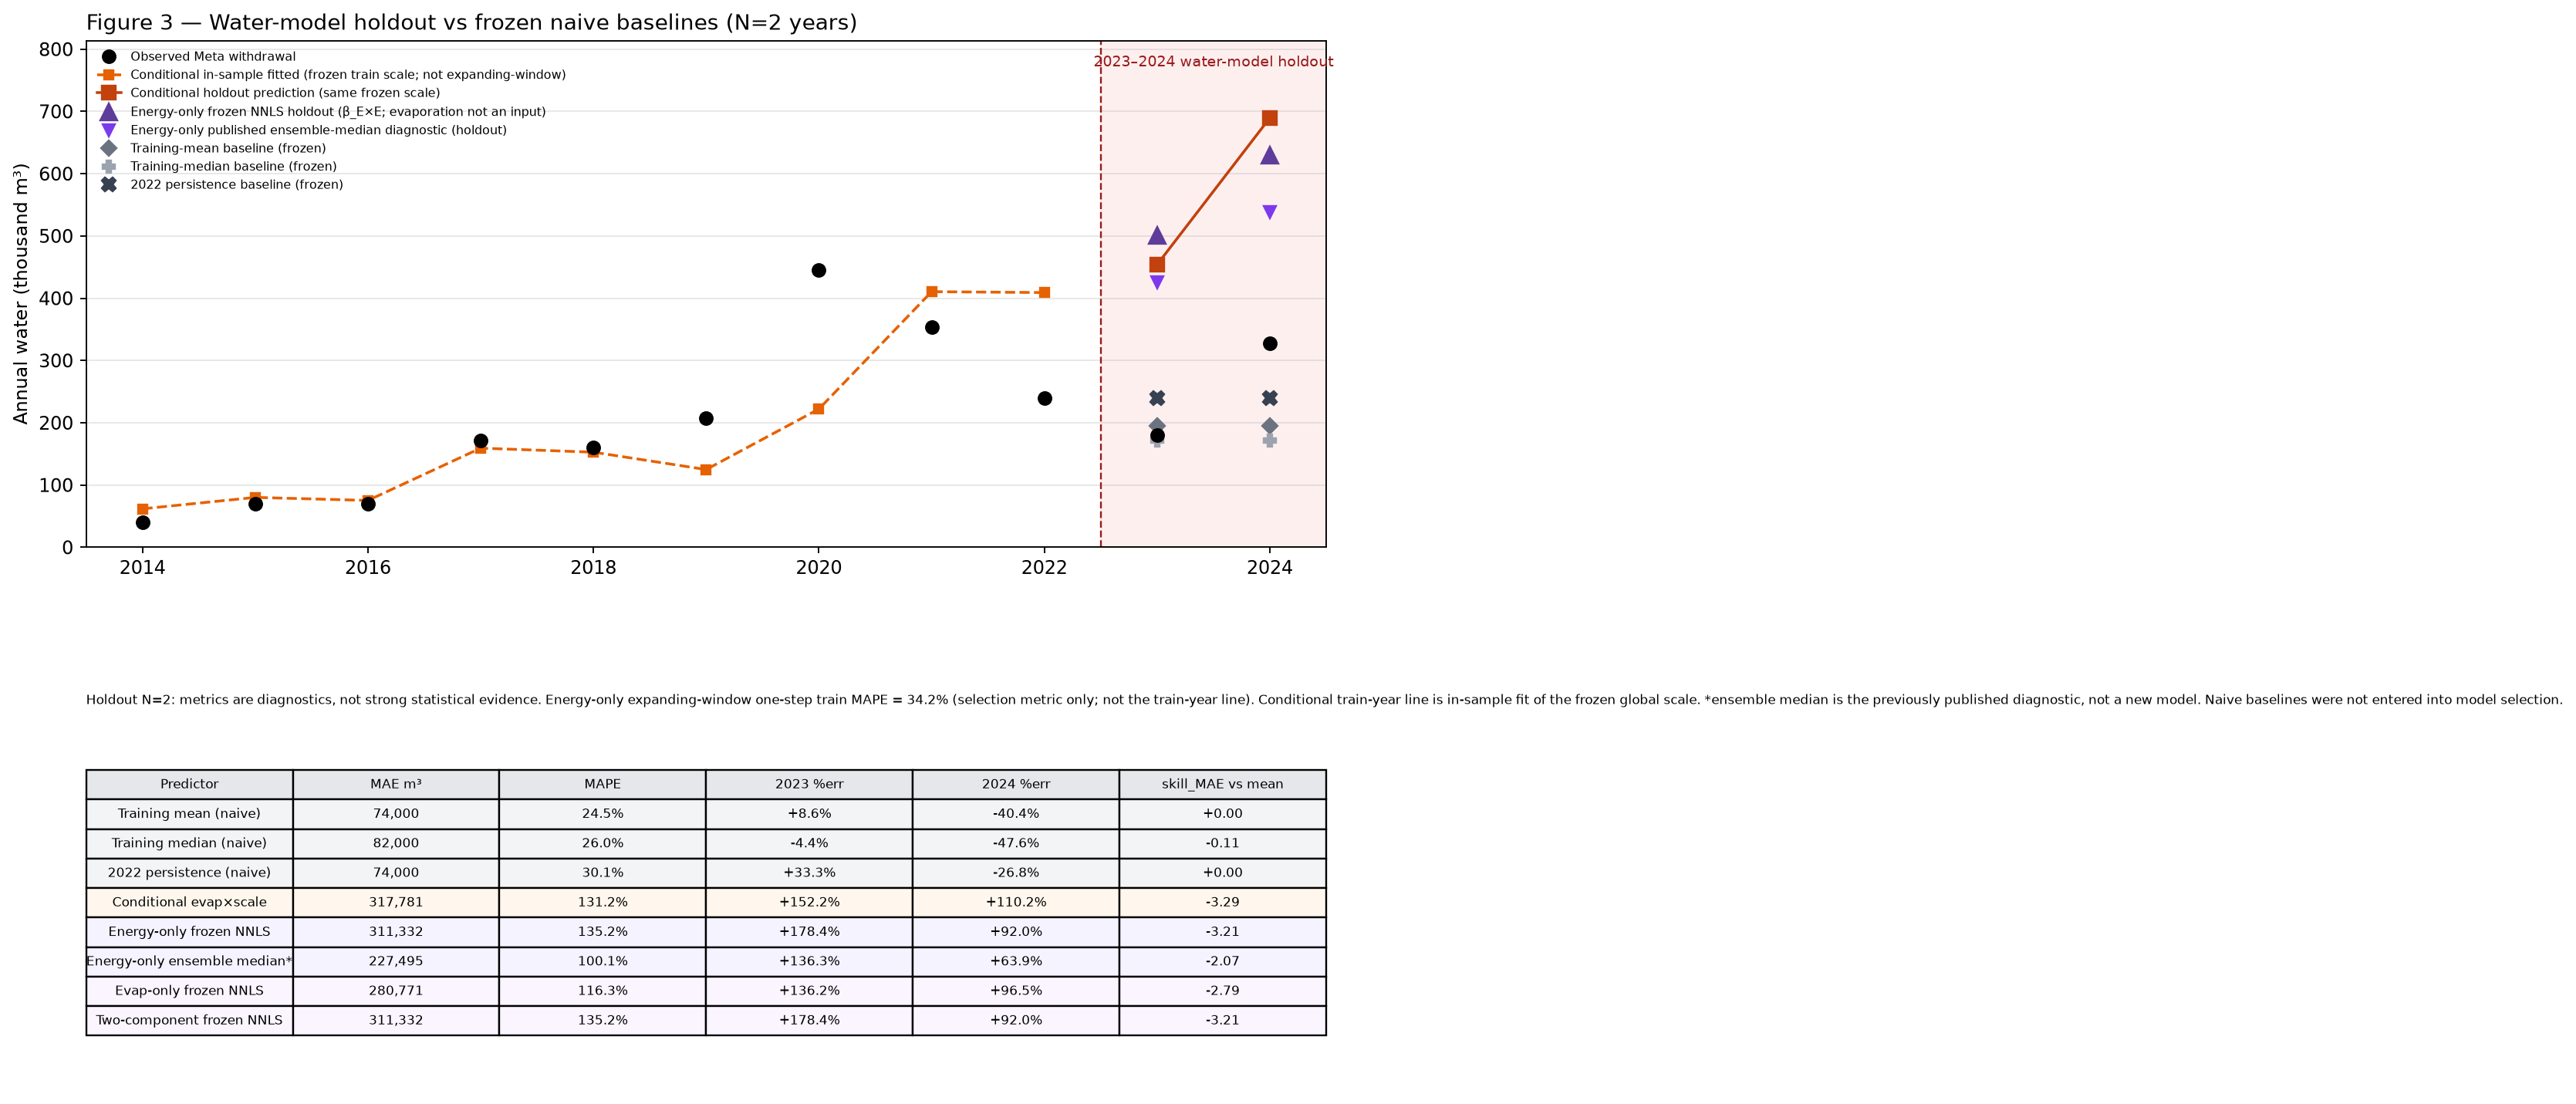
\includegraphics[width=0.8\linewidth]{../../Meta_Prineville_Oregon_v3/outputs/pipeline_report/figures/fig03_water_model_accuracy.png}
    \caption{Annual Meta water validation. The main message is comparative out-of-sample skill: current physics/energy predictors do not beat simple historical references on the two held-out years. \latesttxt{Evidence class: frozen predictive validation; Meta annual campus-withdrawal boundary; holdout (n=2) (2023--2024); units thousand m\(^3\) and percent error. The figure is preserved unchanged and does not identify monthly water, consumption, source share, or mechanism.}}
    \label{fig:water_model_accuracy}
\end{figure}
% \maybegraphic{../outputs/pipeline_report/figures/fig03_water_model_accuracy.png}
% {}

With only two holdout years, this is a small statistical sample. The practical conclusion is nevertheless clear:
\[
\boxed{\text{the current annual water model is a mechanism / falsification baseline, not a reliable predictor}.}
\]

The failure is informative: energy plus simple evaporative weather physics is not sufficient to explain campus withdrawal. Missing drivers may include technology/mode, source/reuse strategy, blowdown, non-cooling use, or other operational changes, but the current data do not identify which one dominates.

\subsection*{\latesttxt{3a. City utility meters convert part of the monthly water problem from modeled to observed}}

\latesttxt{The v2 City integration adds 3,456 meter-month records covering 36 meters from 2012--2026, with 2026 treated as observed only through July. The canonical monthly response is the Facebook Data Center WATER-COMM + ADD'L WATER customer-service component. Bulk/hydrant, SWR METER, WELL METER FOR SEW, Trailer City, and Warehouse are retained separately and excluded from that response because their physical/accounting roles are unresolved.}

\oldtxt{Prior text mixed the native-support baseline MAE (8,035 m\(^3\)) with common-support gray-box metrics; superseded below.}

\latesttxt{On the canonical identical common support (\(n=120\) months across ten complete years within 2014--2024; incomplete 2015 excluded), seasonal persistence is best by MAE (7,473.1 m\(^3\); RMSE 11,164.8 m\(^3\)), while the frozen gray-box evaporation\(\times\)scale candidate has MAE 11,728.1 m\(^3\) and RMSE 15,879.4 m\(^3\). The gray-box retains seasonal-shape signal (pooled within-year-share correlation \(r=0.751\), \(n=132\) shape months) but overconcentrates use in summer: complete-year observed JJA shares span 0.365--0.544 versus 0.751--0.939 for the gray-box. This is an observed City-service validation, not an all-source campus-water validation.}

\latesttxt{Annual reconciliation is diagnostic only: City service is very close to Meta's annual withdrawal in 2022, and City service + bulk is very close in 2023--2024, but that relationship is not stable in earlier years and is not promoted to a physical campus mass-balance identity. WELL METER FOR SEW versus OWRD direct POD has \(n=141\) overlapping reported months and Pearson \(r=0.0929\) (\(n=128\), \(r=0.1397\) when both are nonzero), so no source, master/submeter, or physical identity is asserted.}

\begin{figure}[ht]
    \centering
    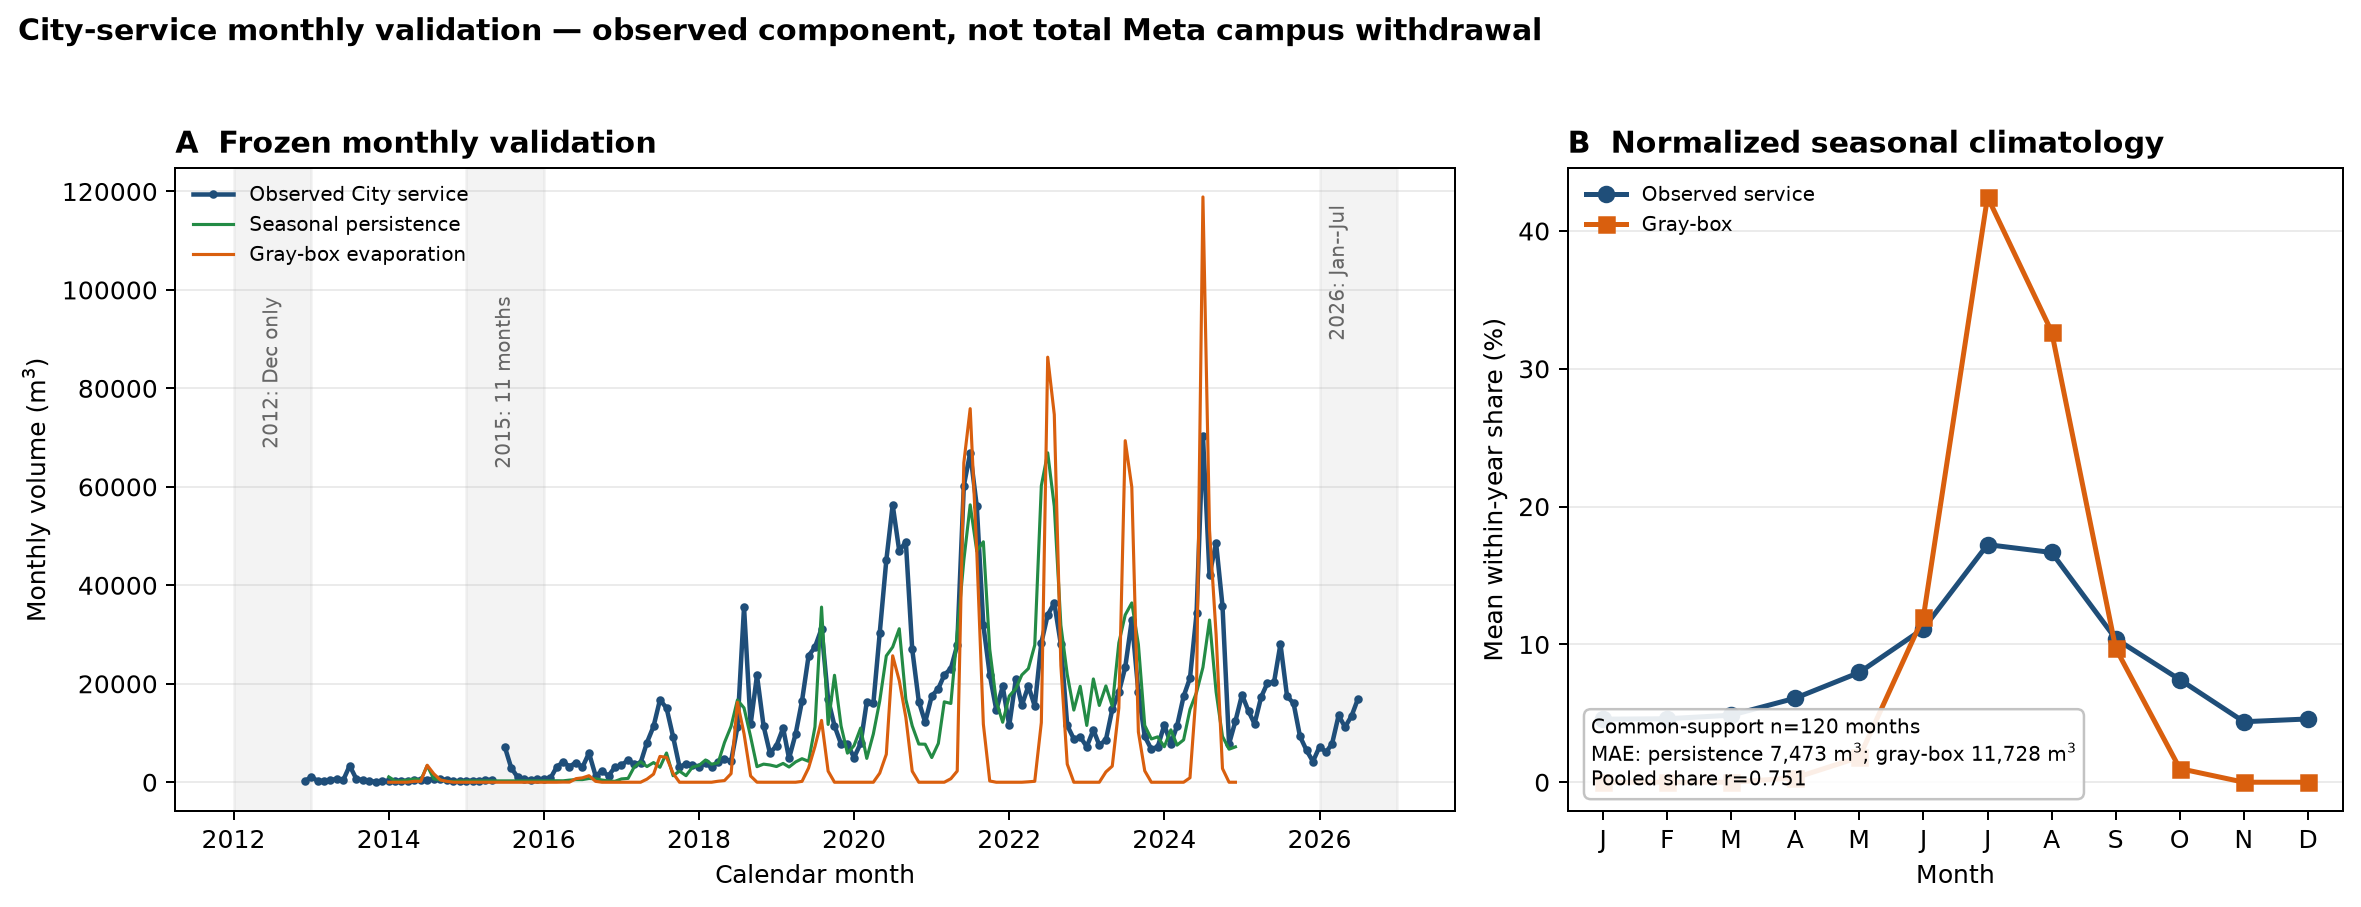
\includegraphics[width=0.98\linewidth]{../../outputs/glossary_refresh_20260903/figures/fig04_city_service_validation.png}
    \caption{\latesttxt{Frozen City-service monthly validation. Panel A compares the OBSERVED City WATER-COMM + ADD'L WATER customer-service component with the strongest frozen simple baseline and the frozen gray-box evaporation candidate; 2012 (December only), 2015 (11 months), and 2026 (January--July) are visibly partial and excluded from the \(n=120\) common-support ranking over ten complete years within 2014--2024. Panel B compares normalized mean within-year share (percent) for observed service and gray-box output. Units are m\(^3\)/month and percent share; scope is City service, not total Meta campus withdrawal.}}
    \label{fig:city_service_validation}
\end{figure}

{\color{purple!85!black}
\begingroup
\footnotesize
\setlength{\tabcolsep}{3pt}
\setlength{\emergencystretch}{3em}
\raggedright
\sloppy
\begin{longtable}{@{}p{0.180\linewidth}p{0.040\linewidth}p{0.100\linewidth}p{0.100\linewidth}p{0.080\linewidth}p{0.110\linewidth}p{0.270\linewidth}@{}}
\caption{Frozen City-service validation metrics on identical common support (n=120 months across ten complete years in 2014--2024; incomplete 2015 excluded). Response is the observed City WATER-COMM + ADD'L WATER service component, not all-source Meta campus withdrawal.}\\
\toprule
\textbf{Model} & \textbf{n} & \textbf{MAE (m3)} & \textbf{RMSE (m3)} & \textbf{SMAPE} & \textbf{Median AE (m3)} & \textbf{Information set} \\
\midrule
\endfirsthead
\toprule
\textbf{Model} & \textbf{n} & \textbf{MAE (m3)} & \textbf{RMSE (m3)} & \textbf{SMAPE} & \textbf{Median AE (m3)} & \textbf{Information set} \\
\midrule
\endhead
\midrule
\multicolumn{7}{r}{\emph{Continued on next page}}\\
\endfoot
\bottomrule
\endlastfoot
Month-of-year climatology & 120 & 9,430.1 & 14,691.6 & 0.862 & 5,173.8 & prospective\_forecastable\_baseline \\
Seasonal persistence & 120 & 7,473.1 & 11,164.8 & 0.631 & 4,672.0 & prospective\_forecastable\_baseline \\
Annual-electricity scale & 120 & 8,692.5 & 12,973.2 & 0.648 & 6,236.8 & contemporaneous\_explanatory \\
Gray-box evaporation scale & 120 & 11,728.1 & 15,879.4 & 1.557 & 8,460.5 & contemporaneous\_explanatory \\
Electricity + evaporation & 120 & 8,518.4 & 12,686.2 & 0.612 & 4,809.5 & contemporaneous\_explanatory \\
\end{longtable}
\endgroup

}

\latesttxt{The water boundaries used by this document are therefore kept explicit in the following main-body accounting table. ``No'' in the automatic-sum column is an identifiability restriction, not an assertion that the physical streams can never be related.}

{\color{purple!85!black}
\begingroup
\scriptsize
\setlength{\tabcolsep}{3pt}
\setlength{\emergencystretch}{3em}
\raggedright
\sloppy
\begin{longtable}{@{}p{0.170\linewidth}p{0.170\linewidth}p{0.200\linewidth}p{0.080\linewidth}p{0.300\linewidth}@{}}
\caption{City/Meta/OWRD water-boundary map. No row may be automatically summed with another without an identified accounting relationship.}\\
\toprule
\textbf{Boundary / source} & \textbf{Canonical quantity} & \textbf{Status / coverage} & \textbf{Auto-sum?} & \textbf{Role / caveat} \\
\midrule
\endfirsthead
\toprule
\textbf{Boundary / source} & \textbf{Canonical quantity} & \textbf{Status / coverage} & \textbf{Auto-sum?} & \textbf{Role / caveat} \\
\midrule
\endhead
\midrule
\multicolumn{5}{r}{\emph{Continued on next page}}\\
\endfoot
\bottomrule
\endlastfoot
Meta annual withdrawal & \path{Q_W_WITH}\newline W\_Meta,y & REPORTED; 2014--2024 (11 annual values) & No & Annual campus disclosure; withdrawal, not consumption; no monthly allocation implied. \\
City WATER-COMM + ADD'L WATER service & \path{Q_CITY_METER_SERVICE}\newline W\_City,service,m & OBSERVED/REPORTED; 2012-12 to 2026-07 (163 observed months; 2012, 2015, and 2026 partial) & No & Customer municipal-service component; model response; not all-source campus withdrawal. \\
City bulk/hydrant & \path{Q_CITY_BULK_WATER} & OBSERVED/REPORTED; 2018-02 to 2026-08 (103 billing months) & No & Billing-month component with unresolved campus/use boundary; service+bulk is diagnostic only. \\
City SWR METER & \path{Q_CITY_SWR_METER} & OBSERVED/REPORTED; identity unresolved; 2012-12 to 2026-07 (163 months) & No & Keep separate; naming/numerical proximity does not establish master/submeter or return semantics. \\
City WELL METER FOR SEW & \path{Q_CITY_WELL_METER_SEW} & OBSERVED/REPORTED; identity unresolved; 2012-12 to 2026-07 (163 months) & No & Weak OWRD-POD correspondence; do not infer source, sewer, or master/submeter identity. \\
OWRD direct Vitesse/Facebook POD & \path{Q_DIRECT_POD} & REPORTED; 2010-10 to 2024-09 (450 reported POD-month rows) & No & Direct-POD reporting boundary; not total Meta withdrawal and not automatically additive to City service. \\
All-source monthly Meta/campus withdrawal & W\_Meta,total,m (coverage/report concept; no distinct registry row) & NOT IDENTIFIED; None & No & Service, bulk, SWR/WELL, direct POD, reuse/return/storage, lifecycle, and campus-scope relations do not close a mass balance. \\
\end{longtable}
\endgroup

}

\subsection*{4. Public regulatory data can reconstruct missing regional grid context}

The FERC-constrained historical PACW proxy agrees well with EIA-930 during the mature 2016--2018 overlap ($r=0.919$, NRMSE $=0.083$). This makes pre-EIA regional demand usable as a \emph{validated proxy}, not as directly observed West-hourly demand.

\subsection*{5. Independent permit evidence proves that facility technology is not temporally static}

Crook County records document a PRN1 addition of approximately \(82.7\)k ft\(^2\) (reported range \(82{,}273\)--\(82{,}736\) ft\(^2\)), IT-serving chilled-water/CRAH/chiller infrastructure, late-2023 commissioning/testing, and an additional chiller operational in early 2024.

This is important because a single cooling architecture over 2011--2024 is a simplification. It is \textbf{not} evidence that the permit event caused the 2023--2024 water-model failure, and it was not used to retune the holdout.

\subsection*{\latesttxt{5a. Cross-site evidence supports structural, not quantitative, transfer}}

\latesttxt{Forest City v3 is a deliberately conservative transportability experiment. Same-window observations show materially different climate, and the weather\(\times\)controller decomposition confirms that cooling-regime occupancy depends jointly on climate and control logic. Yet transferred Lei--Masanet/ESIF calculations are not site calibration: qualitative physics transfer is PARTIAL, quantitative transfer is NOT\_VALIDATED, cooling-water magnitude and effective facility \(\Delta T\) remain UNIDENTIFIED, and \texttt{MODEL\_CALIBRATED=NO}. The acquisition implication is also clear: engineering and utility records now outrank more weather data for improving site calibration.}

\subsection*{6. Groundwater has crossed from ``missing state'' to ``testable empirical layer''}

The GWIS QC step processed 812 records, of which 800 contain numeric BLS measurements. After metadata-based exclusions, 796 are retained as potentially usable groundwater-state observations. Of these, 427 are explicitly STATIC and 369 are retained with ambiguous/unknown status.

Known problematic observations (for example PUMPING, FLOWING, INJECTING, DRY, or NOT MEASURED) are excluded only when metadata justify exclusion; surprising values are not deleted by magnitude alone.

The target is now physically signed:
\[
\text{bls\_anomaly}_{i,t}=BLS_{i,t}-\overline{BLS}_i,
\qquad
\text{head\_anomaly}_{i,t}=-\text{bls\_anomaly}_{i,t}.
\]

Three systems remain \emph{estimation candidates} in the current Task-1 screen---meaning sufficient data to attempt a validated empirical response benchmark, not identified groundwater dynamics:
\[
\boxed{\text{Heliport (SRC-GC), Millican (SRC-JA), Airport \#2 (SRC-GB)}}.
\]
Airport pumping remains the accepted combined SRC-GA+SRC-GB group. The broad parameterized-aquifer model remains Class~B / not ready. No groundwater-response model is fitted.

However, Heliport and especially Millican retain large REPORTED/UNKNOWN excursions that are not explained by available local method/status metadata. Measured groundwater observations are now available and several pumping/well systems contain enough overlap to attempt an empirical benchmark, but measurement-condition uncertainty remains material at some wells. The data are therefore \emph{usable with explicit sensitivity analysis}, not ``fully cleaned.''

% \maybegraphic{../outputs/pipeline_report/figures/fig_advisor_gwis_estimation_candidates.png}

\begin{figure}
    \centering
    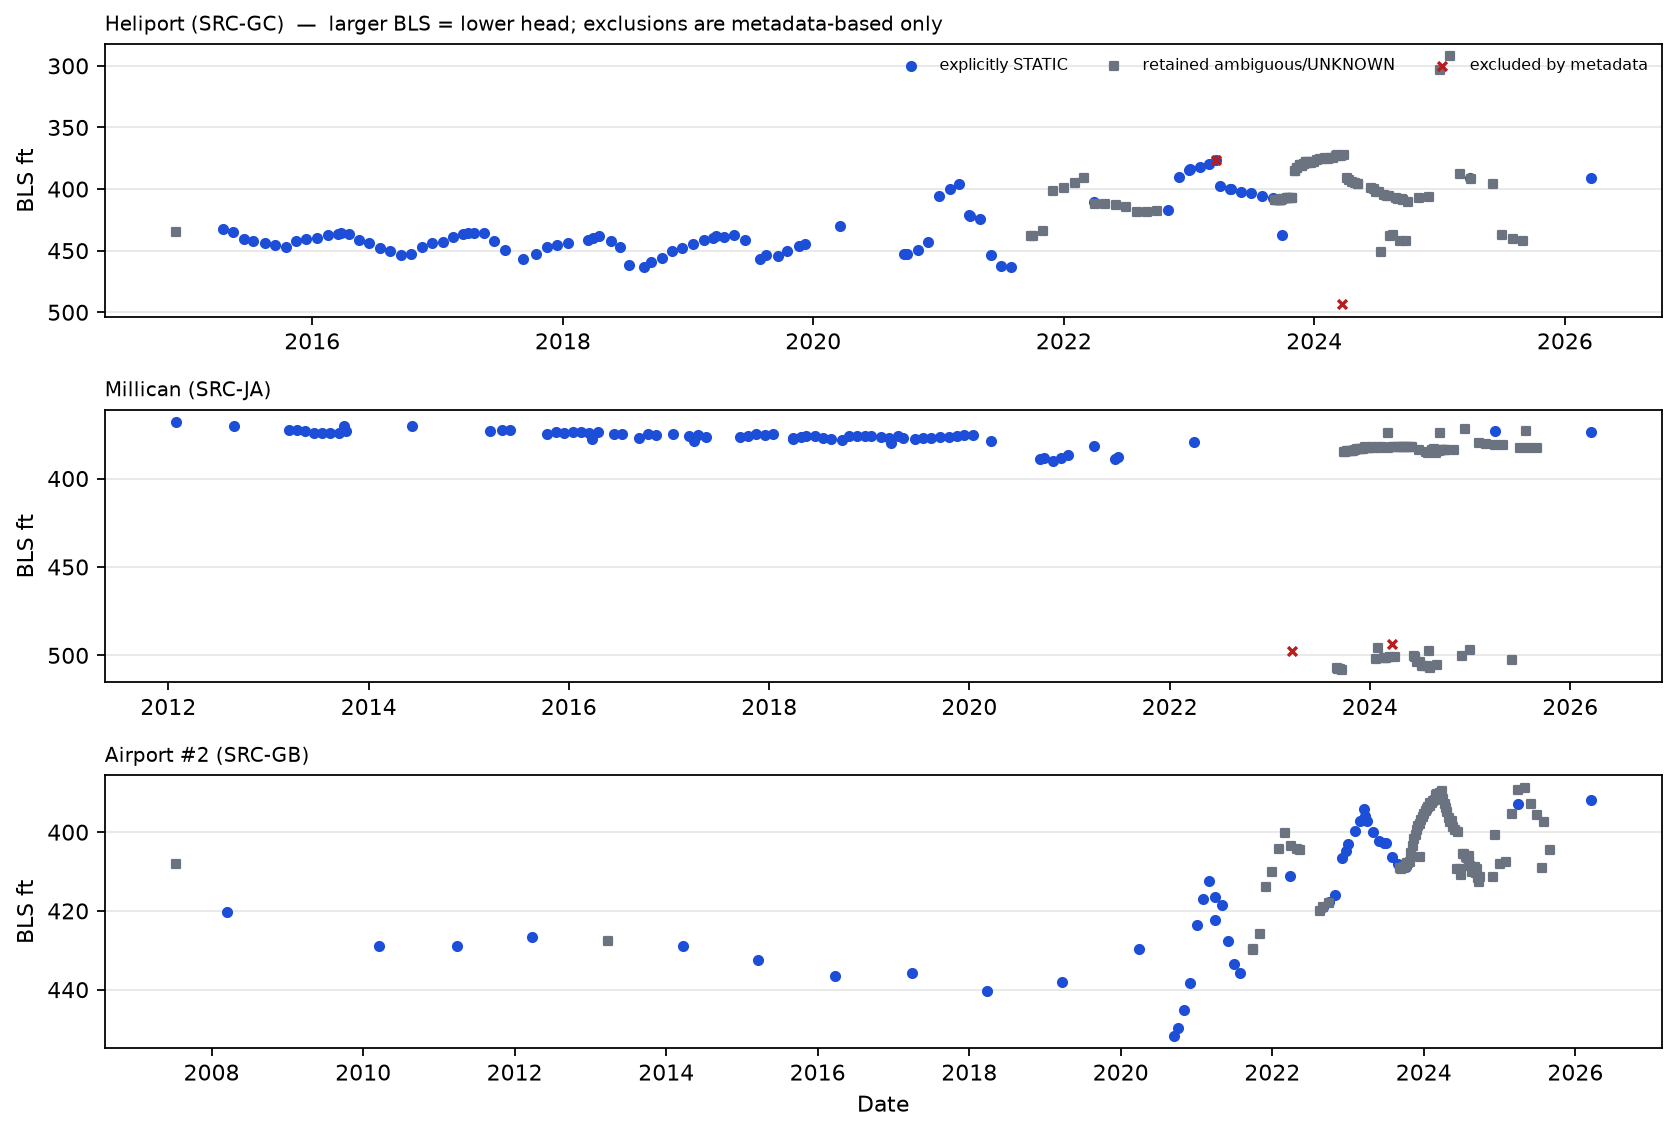
\includegraphics[width=0.8\linewidth]{../../Meta_Prineville_Oregon_v3/outputs/pipeline_report/figures/fig_advisor_gwis_estimation_candidates.png}
    \caption{GWIS BLS at the three estimation-candidate wells. Blue circles are explicitly STATIC; grey squares are retained ambiguous/UNKNOWN; red crosses are metadata exclusions (not magnitude outliers). Larger BLS is lower hydraulic head. \latesttxt{Evidence class: measured/reported GWIS observations; (n=488) plotted records across SRC-GC, SRC-JA, and SRC-GB, of which 483 are state-model eligible; units ft below land surface; individual-well scope. The preserved figure does not establish causal pumping response or a common-datum groundwater field.}}
    \label{fig:gwis_candidates}
\end{figure}
% 

% ================================================================
\section{What should we trust, and what remains unidentified?}
% ================================================================

\subsection*{Confidence ladder}

\begingroup
\small
\begin{longtable}{@{}p{0.20\linewidth}p{0.31\linewidth}p{0.43\linewidth}@{}}
\caption{\latesttxt{Current confidence hierarchy. Confidence attaches to a quantity and boundary, not to a source name in isolation.}}\\
\toprule
\textbf{Level} & \textbf{Components} & \textbf{Interpretation} \\
\midrule
\endfirsthead
\toprule
\textbf{Level} & \textbf{Components} & \textbf{Interpretation} \\
\midrule
\endhead
High-confidence evidence & Meta annual ground truth; canonical NOAA weather; EIA modern grid; OWRD reported pumping; permit chronology; GWIS observations as observations & Use directly at their stated physical/accounting boundaries. \\
\latesttxt{Observed City-service component} & \latesttxt{Facebook Data Center WATER-COMM + ADD'L WATER monthly utility-meter report; 2012--2026 with 2026 through July} & \latesttxt{Use as an observed customer-service boundary only. It does not close monthly campus withdrawal, source shares, sewer return, reuse, or groundwater forcing.} \\
\oldtxt{Externally validated facility structure} & \oldtxt{M100: IT/facility/cooling accounting; weather-dependent cooling overhead; nonconstant derived PUE; persistent temporal structure} & \oldtxt{Use as structural constraints only. Do not transfer M100 coefficients, cooling fractions, control thresholds, or water quantities.} \\
\oldtxt{External facility-validation stack} & \oldtxt{M100 structure; Lei--Masanet climate/technology intensity audit; preliminary Frontier IT-load/accessory-power validation} & \oldtxt{Use M100 as frozen structural evidence; treat Lei--Masanet as an intensity/archetype backbone only if the annual/RNG gate passes; treat Frontier result as preliminary until gap-safe QC closes. No generic coefficient transfer.} \\
\latesttxt{Closed/strong external structural evidence} & \latesttxt{M100 frozen structure; Frontier corrected load-dependence result} & \latesttxt{Use as model-form constraints at their boundaries; do not transfer site coefficients or water quantities.} \\
\latesttxt{Partial / transfer-restricted evidence} & \latesttxt{Lei--Masanet final PARTIAL closure; ESIF electrical PARTIAL closure; Forest City qualitative transfer PARTIAL} & \latesttxt{Use for archetype structure, regime/state allowance, and falsification. No quantitative generic adapter or cross-site coefficient transfer is validated.} \\
\latesttxt{Bounded compute-component evidence} & \latesttxt{Modern AI IT-power layer: frozen workload/mode/scale-conditioned CPU/H100 results} & \latesttxt{Use for bounded compute scenarios. Full-node AC, other-node power, production mix, and facility-IT aggregation remain explicit uncertainties.} \\
Validated proxy / reconstruction & FERC historical PACW bridge; annual-closed facility-electricity profile & Useful because constraints/overlap validation are explicit; not raw telemetry. \\
Mechanism / scenario & cooling gray-box; stochastic workload; monthly water allocations; temporal carbon/water scenarios & Useful for sensitivity and counterfactuals, not historical identification. \\
Weak predictor & annual campus-water models & No demonstrated holdout advantage over naive references. \\
\latesttxt{Weak monthly physical predictor} & \latesttxt{City-service gray-box level model} & \latesttxt{Seasonal persistence beats weather/evaporation models on MAE; gray-box shares are too summer-peaked. Use as mechanism/falsification evidence, not a promoted predictor.} \\
\oldtxt{Not yet identified} & \oldtxt{hourly Meta IT; monthly campus meters; exact source shares; pumping-to-head causal response; aquifer dynamics; exact serving generators/marginal impacts; costs/optimization} & \oldtxt{Requires new identification or data before strong claims/optimization.} \\
\latesttxt{Not yet identified} & \latesttxt{hourly Meta IT; all-source monthly campus withdrawal; source/return/reuse shares; generic quantitative PUE/WUE adapter; pumping-to-head causal response; aquifer dynamics; exact serving generators/marginal impacts; coupled planning/policy result} & \latesttxt{Requires source-accounting or response identification before strong coupled-planning claims.} \\
\bottomrule
\end{longtable}
\endgroup

\begin{center}
\fbox{\parbox{0.94\linewidth}{
\latesttxt{\textbf{Current project bottom line.} Facility-model structure is sufficiently constrained for reduced planning representations, but generic numerical transfer is not validated. The observed monthly City-service component shifts the water problem from ``invent a monthly shape'' to source/boundary accounting. The sequential critical path is \(W^{cond}\rightarrow\{W^{with},W^{return},\text{source share}\}\rightarrow q^{gw}\), then \(q^{gw}+\{R,\text{background hydrology}\}\rightarrow h\), and finally deterministic \(M_0\)-versus-\(M_1\) decision replay.}
}}
\end{center}

\subsection*{Missing information by the scientific relationship it blocks}

\begin{center}
\scriptsize
\begin{tabularx}{\linewidth}{@{}p{0.22\linewidth}p{0.34\linewidth}Y@{}}
\toprule
\textbf{Relationship we want} & \textbf{Main missing / uncertain information} & \textbf{What it prevents today} \\
\midrule
\oldtxt{Workload / hardware \(\rightarrow\) facility IT} & \oldtxt{Modern AI workload--power mapping and server/node-to-facility boundary parameters} & \oldtxt{Generic \(P^{IT}\) scenarios; NLR/H100/B200/MLPerf source audit and smallest experiment are designed but not yet validated.} \\
\latesttxt{Workload / hardware \(\rightarrow\) facility IT} & \latesttxt{Full-node AC/other-node power, production workload mix, network/storage/service/idle load, and same-system aggregation evidence} & \latesttxt{The compute component is bounded, but a closed facility-IT scenario still requires explicit node/system/facility uncertainty.} \\
\oldtxt{IT + weather + technology \(\rightarrow\) cooling power} & \oldtxt{Cross-technology archetype parameters and independent facility validation} & \oldtxt{Generic \(f_k\) calibration; next sources are Lei--Masanet/LBNL and Frontier.} \\
\oldtxt{IT + weather + technology \(\rightarrow\) facility energy / conditioning water} & \oldtxt{Annual Lei--Masanet envelope reproducibility, hidden-RNG stability, and clean adapter semantics; Frontier gap-safe QC} & \oldtxt{Whether \(PUE_k(\mathbf w,\theta_k)\) and \(WUE_k(\mathbf w,\theta_k)\) can become the planning archetype backbone.} \\
\latesttxt{IT + weather + architecture/state \(\rightarrow\) facility overhead} & \latesttxt{Validated quantitative parameterization that survives facility epochs; ESIF shows stationary IT+weather alone is insufficient} & \latesttxt{A universal numerical overhead law. For planning, retain bounded/archetype scenarios unless new independent evidence supports transferable coefficients.} \\
\latesttxt{Climate/technology \(\rightarrow\) facility conditioning-water intensity} & \latesttxt{Quantitative generic adapter remains unavailable because Lei--Masanet promotion is blocked; cross-site transfer is not validated} & \latesttxt{Use the \(W^{cond}=E^{IT}WUE_k\) structure as a model class, not as a validated universal parameterization.} \\
\oldtxt{Workload \(\rightarrow\) IT / facility operation} & \oldtxt{workload telemetry, IT power, detailed cooling state/control} & \oldtxt{Historical hourly internal-state identification; this row is subsumed by the boundary-specific workload/hardware row above.} \\
\oldtxt{Cooling \(\rightarrow\) campus water} & \oldtxt{monthly campus water, consumption vs withdrawal, discharge/return, cooling-loop operation, source/reuse shares} & \oldtxt{Reliable subannual water prediction and source-resolved accounting.} \\
\oldtxt{Conditioning water \(\rightarrow\) source withdrawal / consumption / return} & \oldtxt{Campus source shares, municipal/direct-well delivery, reuse/reclaimed water, discharge/return, blowdown destination, storage/ASR accounting; City-service is observed, but bulk/SWR/WELL/direct-POD/return/source relationships remain unresolved.} & \oldtxt{Groundwater forcing cannot yet be mapped.} \\
\latesttxt{\(W^{cond}\rightarrow W^{with}/W^{return}/\)source share \(\rightarrow q^{gw}\)} & \latesttxt{Service/bulk/SWR/WELL/direct-POD crosswalk; withdrawal-versus-consumption/return; reuse, blowdown, storage/ASR, meter lifecycle, and campus-scope accounting} & \latesttxt{An identified site-water mass balance and groundwater forcing series. City service alone does not close either quantity.} \\
\oldtxt{Pumping \(\rightarrow\) groundwater} & \oldtxt{measurement-condition uncertainty, recharge/background hydrology, other pumping; physical \(T,S,S_y\) for full model} & \oldtxt{Causal/physical groundwater response and aquifer simulation.} \\
\latesttxt{\(q^{gw}+\) recharge/background \(\rightarrow\) groundwater response} & \latesttxt{Chronological response validation, measurement-condition uncertainty, recharge/background hydrology, other pumping; physical \(T,S,S_y\) for a later full model} & \latesttxt{A validated empirical head-response benchmark; no pumping-to-groundwater response is presently identified.} \\
Facility load \(\rightarrow\) grid externality & actual supply contract/serving attribution, marginal dispatch response & Meta-specific marginal carbon/water consequences. \\
\latesttxt{Validated response functions \(\rightarrow M_0\) vs \(M_1\) decisions} & \latesttxt{Closed source/GW forcing and response, workload flexibility, tariffs/costs, capacity constraints, and predeclared decision metrics} & \latesttxt{Credible replay of whether dynamic source/GW representation changes siting, technology/source choice, equity, or regret.} \\
\bottomrule
\end{tabularx}
\par\smallskip{\small\itshape The important gaps are causal/identification gaps, not simply a list of missing files.\par}\end{center}

% ================================================================
\section{What simulation can and cannot do today}
% ================================================================

Simulation is useful when its role is explicit.

\textbf{Useful now:}
\begin{itemize}
\item explore plausible workload shapes and utilization patterns;
\item \oldtxt{propagate IT load and weather through explicitly labeled facility/cooling archetypes, with PUE derived as an output;} \newtxt{propagate variable IT load through validated climate--technology intensity archetypes, with energy-weighted PUE/WUE and explicit conditioning-water components;}
\item compare explicit subannual water-allocation scenarios;
\item study timing interactions with regional carbon signals;
\item test future counterfactual technology/source/operating assumptions.
\end{itemize}

\textbf{Not justified now:}
\begin{itemize}
\item recovering Meta's historical workload or hourly IT telemetry;
\item \oldtxt{reconstructing actual monthly campus water without a meter/stronger model;} \latesttxt{recovering all-source monthly Meta campus withdrawal from the observed City-service component; the service boundary is observed, but the total/source/return balance remains unidentified;}
\item interpreting simulated pumping as the cause of an observed groundwater movement;
\item treating scenario output as evidence of an actual historical cooling mode or source share;
\item \newtxt{transferring M100 coefficients, free-cooling thresholds, cooling fractions, or circulating liquid flow as generic facility/water parameters;}
\item \newtxt{equating Lei--Masanet conditioning-water use/WUE with source withdrawal, consumption, or groundwater pumping.}
\item \latesttxt{treating Forest City transferred Masanet/ESIF outputs as site calibration, or treating ESIF/M100 coefficients and regime thresholds as generic facility parameters;}
\end{itemize}

% ================================================================
\section{Immediate next scientific decision}
% ================================================================

\oldtxt{The next step was framed as one narrow groundwater-only empirical question.}

\oldtxt{\textbf{Updated sequencing after M100.} The immediate facility-model task is to validate climate--technology response surfaces for cooling power, withdrawal, and consumption (Lei--Masanet/LBNL), with Frontier as an independent thermal benchmark; the modern workload/hardware block can proceed in parallel.}

\oldtxt{\textbf{Current sequencing.} The first Lei--Masanet audit is complete. The immediate facility gate is the predeclared annual PUE/WUE-envelope reproduction plus hidden-RNG test and Frontier gap-safe QC. If it passes, freeze a clean planning adapter \(P^{fac}=P^{IT}PUE_k(\mathbf w,\theta_k)\), \(W^{cond}=E^{IT}WUE_k(\mathbf w,\theta_k)\); if it fails, retain Lei--Masanet only as qualitative archetype evidence. In parallel, the modern workload/hardware \(\rightarrow P^{IT}\) experiment is designed, and the pumping\(\rightarrow\)groundwater benchmark remains a separate Thrust-A identification task.}

\oldtxt{\textbf{Current critical path.} The main bottleneck is no longer another facility-model search. M100 and Frontier are closed; ESIF's electrical layer is closed PARTIAL; Lei--Masanet is closed PARTIAL with adapter promotion blocked; Forest City v3 does not validate quantitative transfer. The two immediate scientific tasks are therefore parallel: reconcile the observed City-service/bulk/SWR/WELL/direct-POD evidence and run the pumping\(\rightarrow\)groundwater benchmark. Modern AI \(P^{IT}\) validation remains a supporting track.}

\latesttxt{\textbf{Current critical path.} The closed external-validation stack removes further generic facility-model search from the critical path. The work is now sequential: \textbf{(1)} reconcile site-water/source accounting from City service, bulk, SWR/WELL, direct POD, meter lifecycle, reuse/return/blowdown, and scope evidence without forcing closure; \textbf{(2)} translate the identified source shares into groundwater forcing \(q^{gw}\); \textbf{(3)} validate groundwater response using pumping plus recharge/background controls; and \textbf{(4)} replay the smallest deterministic source/GW-aware \(M_1\) against static \(M_0\). The modern IT-power layer is already frozen bounded and remains a supporting uncertainty block, not the immediate bottleneck.}

\[
\boxed{\parbox{0.90\linewidth}{\centering
\latesttxt{Groundwater-response stage (after forcing is defensible): does antecedent pumping add stable chronological predictive information about groundwater levels beyond seasonality, recharge/background hydrology, and trend?}}}
\]

To align monthly OWRD pumping with uneven GWIS measurement density, the first benchmark should use one target per well-month (for example, the median eligible head anomaly in that month).

Two samples should be pre-specified:

\[
\textbf{Primary: all metadata-eligible observations},
\]
\[
\textbf{Sensitivity: explicitly STATIC observations only}.
\]

For SRC-GC, SRC-JA, and SRC-GB (with Airport pumping kept as the accepted combined SRC-GA+SRC-GB group), compare:

\[
M_0:
\tilde h_{i,m}
=
\alpha_i+s_i(month_m)+\gamma_i m+\epsilon_{i,m},
\]

against

\[
M_1:
\tilde h_{i,m}
=
\alpha_i+s_i(month_m)+\gamma_i m+\beta_iX^{antecedent\,pumping}_{i,m}+\epsilon_{i,m}.
\]

Use only completed prior-month pumping exposures; no same-month total that can contain pumping after the groundwater measurement. Validation should be chronological, not random.

\textbf{Decision rule:}

\[
\boxed{\text{Stable incremental skill} \Rightarrow \text{build a small reduced-order groundwater module.}}
\]
\[
\boxed{\text{No stable incremental skill} \Rightarrow \text{add recharge/background controls before more complexity.}}
\]

Only after the response models are credible should the project move toward coupled workload/source/siting optimization.

\todo[inline]{Ultimate fidelity test: compare the static PSCC-style \(M_0\) against the smallest empirically defensible source-resolved/groundwater \(M_1\). Add higher-fidelity facility dynamics only if decision replay shows material regret, changed choices, or constraint violations.}

% ================================================================
\section{Discussion questions for the meeting}
% ================================================================

The most useful advisor feedback is not on implementation detail, but on the modeling hierarchy:

\begin{enumerate}
\item Is the overall causal chain the right research abstraction: compute \(\rightarrow\) facility \(\rightarrow\) grid/water \(\rightarrow\) environmental state \(\rightarrow\) decision?
\item Is Prineville now sufficiently grounded to serve as the empirical validation case, despite missing internal telemetry?
\item \oldtxt{Should the next identification effort prioritize groundwater response, or is there a higher-value missing relationship (for example monthly campus water/source shares)?}
\oldtxt{Is the next model-validation priority correctly split between generic facility energy/water archetypes and modern AI \(P^{IT}\), and the parallel pumping-to-groundwater response benchmark?}
\oldtxt{If the current Lei--Masanet annual/RNG gate passes, is the IT-normalized climate--technology intensity model the right planning fidelity, with higher-fidelity part-load/dynamic cooling added only when it changes decisions?}
\oldtxt{Given that quantitative Lei--Masanet promotion is blocked and Forest City numerical transfer is not validated, should the first coupled planner use bounded/archetype facility scenarios while prioritizing the now-observed City-service/source accounting bridge?}
\oldtxt{Once the source bridge and pumping-response benchmark are resolved, is that sufficient evidence to build the first deterministic \(M_1\) for direct comparison against the static PSCC \(M_0\)?}
\item \latesttxt{Is the sequential critical path correct: site-water/source accounting \(\rightarrow q^{gw}\rightarrow\) groundwater response \(\rightarrow M_0\)-versus-\(M_1\) replay?}
\item \latesttxt{What minimum source-accounting and groundwater-response validation gates are sufficient before the first deterministic \(M_1\) decision replay?}
\item Is the proposed progression---simple empirical response \(\rightarrow\) reduced-order state model \(\rightarrow\) later physical/optimization coupling---the right level of complexity?
\item Which eventual decision problem is most scientifically valuable: operations, source selection, siting, or multi-sector water allocation?
\end{enumerate}

\latesttxt{\textbf{Document governance.} This file is the advisor-facing glossary, traceability map, and evidence companion. The canonical project-wide scientific argument and research path remain in \path{main_documents/master.tex}; machine-readable/site-specific truth remains in the Prineville registries and experiment status artifacts. This separation is intentional so that the glossary does not become a second competing source of truth.}

% ================================================================
\appendix
\section{Complete source traceability}
\label{app:sources}

\oldtxt{The table below is generated from the current \emph{Prineville} pipeline source catalog (\SourceCount{} products). It is reference material, not meeting narration.} \oldtxt{External validation datasets such as M100 and Frontier are tracked separately from this site-specific source count.}

\oldtxt{Current public \texttt{main} identifies the Prineville package as Baseline v2. The generated v2 report lists 50 Prineville source products, 82 quantities, and 26 registered methods/models; the validated City-integration run reported 126 package tests PASS. The longtable below preserves the prior generated catalog presentation.}

\latesttxt{At \texttt{08b0c112d8883eb4d23bb05d0d40e1a42c863593}, deterministic reporting regenerates 50 Prineville source products, 82 quantities, and 26 registered methods/models byte-for-byte from the executable catalogs and frozen result claims. The rendered appendices below are generated from those current registries. External validation datasets remain outside the Prineville site-source count.}

\newtxt{External model-validation sources are tracked separately from the site-specific count because their role is structural/archetype validation rather than Prineville measurement:}

\begin{center}
\scriptsize
\begin{tabularx}{\linewidth}{@{}p{0.22\linewidth}p{0.34\linewidth}Y@{}}
\toprule
\textbf{External source} & \textbf{Experiment / role} & \textbf{Current status} \\
\midrule
\newtxt{M100 ExaData \cite{m100exadata}} & \newtxt{Measured IT/facility/cooling/weather structure; node\(\rightarrow\)facility boundary; temporal diagnostics} & \newtxt{Closed/frozen structural benchmark.} \\
\oldtxt{Lei--Masanet 2022 + public code \cite{lei2022}} & \oldtxt{Climate--technology PUE/WUE archetypes; explicit conditioning-water components; annual 50-LHS\(\times\)8760 reproduction} & \oldtxt{First audit complete; bounded annual/RNG validation running.} \\
\latesttxt{Lei--Masanet 2022 + public code \cite{lei2022}} & \latesttxt{Climate--technology PUE/WUE structure and conditioning-water components} & \latesttxt{Final reproducibility closure PARTIAL; quantitative adapter promotion NO/blocked; closed absent new upstream evidence.} \\
\oldtxt{Frontier \cite{frontier2024}} & \oldtxt{Independent compute/accessory-power and liquid thermal context} & \oldtxt{First chronological load-dependence result positive; gap-safe QC correction running.} \\
\latesttxt{Frontier \cite{frontier2024}} & \latesttxt{Independent compute/accessory-power and liquid thermal context} & \latesttxt{Corrected expected-time-grid audit CLOSED; load-dependence conclusion unchanged.} \\
\latesttxt{NLR/ESIF HPC Facility PUE Data \cite{esifdata}} & \latesttxt{Measured IT + facility-overhead components + weather; protected TEST} & \latesttxt{Electrical facility-overhead layer PARTIAL / closed; stationary IT+weather total-aux hypothesis FAIL.} \\
\latesttxt{Forest City v3 project experiment} & \latesttxt{Cross-site climate/controller robustness and transferred-model replay} & \latesttxt{Qualitative physics transfer PARTIAL; quantitative transfer NOT\_VALIDATED; model calibrated = NO.} \\
\oldtxt{NLR / H100--B200 / MLPerf} & \oldtxt{Planned modern workload/device/node/system \(\rightarrow P^{IT}\) validation} & \oldtxt{Source audit + smallest experiment designed; no result yet.} \\
\latesttxt{NLR/H100 + independent public IT-power evidence} & \latesttxt{Workload/mode/scale-conditioned compute-component power and temporal profiles} & \latesttxt{Frozen bounded with explicit node uncertainty; full-node AC and facility-IT bridge incomplete.} \\
\bottomrule
\end{tabularx}
\end{center}

% Superseded hand-maintained source table retained in source history only.
\iffalse
\begingroup
\scriptsize
\setlength{\tabcolsep}{3pt}
\setlength{\emergencystretch}{3em}
\raggedright
\sloppy
\begin{longtable}{@{}p{0.18\linewidth}p{0.25\linewidth}p{0.25\linewidth}p{0.20\linewidth}@{}}
\caption{Complete source-product inventory from the current pipeline catalog. Each row preserves source identity, acquisition route, coverage, physical/accounting boundary, model role, and the main limitation.}\\
\toprule
\textbf{Provider / product} & \textbf{Acquisition + coverage} & \textbf{Boundary + model role} & \textbf{Main limitation} \\
\midrule
\endfirsthead
\toprule
\textbf{Provider / product} & \textbf{Acquisition + coverage} & \textbf{Boundary + model role} & \textbf{Main limitation} \\
\midrule
\endhead
\midrule
\multicolumn{4}{r}{\emph{Continued on next page}}\\
\endfoot
\bottomrule
\endlastfoot
Meta / Facebook\newline \textit{Facebook Sustainability Data 2014} & \url{https://sustainability.atmeta.com/asset/2014-sustainability-data-disclosure/}\newline \textit{Coverage:} 2011-2014 vintage audit / annual / Prineville campus (site table) & \textit{Boundary:} Prineville campus (site table)\newline \textit{Role:} historical source-vintage audit; first 2014 water disclosure & Not the canonical later-year series; site totals are not hourly IT telemetry.\\
Meta / Facebook\newline \textit{2015 Sustainability Data Disclosure} & \url{https://sustainability.atmeta.com/asset/2015-sustainability-data-disclosure/}\newline \textit{Coverage:} 2011-2015 vintage; 2012 location Scope 2 used in canonical table / annual / Prineville ca\ldots & \textit{Boundary:} Prineville campus (site table)\newline \textit{Role:} source-vintage audit; supplies 2012 location Scope 2 & Annual corporate site table, not meters.\\
Meta / Facebook\newline \textit{2016 Sustainability Data Disclosure} & \url{https://sustainability.atmeta.com/asset/2016-sustainability-data-disclosure/}\newline \textit{Coverage:} canonical early electricity (2011-2016); early water; Scope 2 / annual / Prineville campu\ldots & \textit{Boundary:} Prineville campus (site table)\newline \textit{Role:} canonical early electricity, water, location Scope 2, operational GHG & Site annual totals. Do not treat as hourly IT workload.\\
Meta / Facebook\newline \textit{Facebook Sustainability Data 2019} & \url{https://sustainability.atmeta.com/asset/fb_sustainability-data-disclosure-2019/}\newline \textit{Coverage:} canonical 2017-2019 electricity; 2015-2019 water; Scope 2 / annual / Prineville campus (s\ldots & \textit{Boundary:} Prineville campus (site table)\newline \textit{Role:} canonical mid-period electricity, water, location Scope 2 & Site annual totals. Operational GHG definitions are vintage-sensitive.\\
Meta\newline \textit{Meta 2025 Environmental Data Index (FY2024)} & \url{https://sustainability.atmeta.com/wp-content/uploads/2025/10/Meta_2025-Environmental-Data-Index.pdf}\newline \textit{Coverage:} 2020-2024 electricity, water withdrawal, location Scope 2, operational GHG / annual / Pri\ldots & \textit{Boundary:} Prineville campus (site table)\newline \textit{Role:} canonical recent campus electricity, withdrawal, location Scope 2 & Withdrawal is the disclosed site water quantity; consumption vs withdrawal is not separat\ldots\\
Meta\newline \textit{Meta 2023 Environmental Data Index (methods)} & \url{https://sustainability.atmeta.com/wp-content/uploads/2023/07/Meta-2023-Environmental-Data-Index.pdf}\newline \textit{Coverage:} WUE / withdrawal / consumption estimation definitions / methods through 2022 / company/si\ldots & \textit{Boundary:} company/site methodology\newline \textit{Role:} definition/methods context for WUE and water accounting & Canonical numeric series come from 2016/2019/2025 vintages via build\_targets.py, not this\ldots\\
Meta Engineering\newline \textit{Designing a Very Efficient Data Center (2011-04-14)} & \url{https://engineering.fb.com/2011/04/14/core-infra/designing-a-very-efficient-data-center/}\newline \textit{Coverage:} 2011 initial full-load PUE 1.07 and WUE 0.31 L/kWh; outside-air evaporative cooling; no c\ldots & \textit{Boundary:} Prineville initial design\newline \textit{Role:} epoch-1 physics prior and PUE/WUE falsification point & Design point, not measured annual PUE/WUE. Gray-box fan/other fractions are code priors,\ldots\\
Meta\newline \textit{Facebook's Prineville Data Center is Growing Again} & \url{https://datacenters.atmeta.com/2021/03/facebooks-prineville-data-center-is-growing-again/}\newline \textit{Coverage:} 2010 groundbreaking; 2021-03-18 expansion announcement (\textasciitilde{}900,000 sq ft; 11 buildings / \textasciitilde{}4\ldots & \textit{Boundary:} campus\newline \textit{Role:} candidate capacity-state annotation only; completion dates not identified & Announcement is not a commissioning date or MW capacity series.\\
City of Prineville\newline \textit{Economic Opportunities Analysis (2026 draft)} & \url{https://cityofprineville.com/sites/default/files/fileattachments/city_council/page/19317/final_draft_prineville_eoa_january_22_2026.pdf}\newline \textit{Coverage:} 2010-2024; 11 data-center buildings constructed / planning/event / city / campus & \textit{Boundary:} city / campus\newline \textit{Role:} end-state campus-scale cross-check & Does not identify individual commissioning dates or MW.\\
City of Prineville\newline \textit{City Water/Sewer system description} & \url{https://www.cityofprineville.com/1426/WaterSewer}\newline \textit{Coverage:} current / current description / municipal system & \textit{Boundary:} municipal system\newline \textit{Role:} context for municipal ownership, wells/reservoirs, metering & \oldtxt{Not a production time series. Monthly Meta delivery is not in this pipeline.} \latesttxt{System webpage is still not a production time series. Separate 2026 public-records files now provide observed monthly Facebook customer-service meter usage, but not all-source campus withdrawal.}\\
City of Prineville\newline \textit{2024 Consumer Confidence Report} & \url{https://www.cityofprineville.com/DocumentCenter/View/516/2024-Consumer-Confidence-Report}\newline \textit{Coverage:} 2024; groundwater-only source statement / annual/system / PWS 00682 & \textit{Boundary:} PWS 00682\newline \textit{Role:} named well inventory / groundwater-only statement & Not monthly production. Not Meta campus delivery.\\
City of Prineville\newline \textit{Public-records request mechanism} & \url{https://www.cityofprineville.com/1294/Public-Records}\newline \textit{Coverage:} current request mechanism & \textit{Boundary:} \newline \textit{Role:} \oldtxt{documented route for monthly Meta water, discharge, ASR/head (not acquired)} \latesttxt{acquisition route; customer utility-meter package acquired, while wastewater/discharge, municipal-well production/ASR and campus-total closure remain active gaps} & \oldtxt{No monthly Meta water/discharge/ASR operational series is in the repository.} \latesttxt{Monthly City customer-service water is now observed; all-source monthly campus withdrawal, wastewater return, municipal-well production, and ASR operations are still not identified.}\\
\latesttxt{City of Prineville\newline \textit{Facebook utility-meter consumption public records}} & \latesttxt{Immutable 2026 public-records package; 2012--2026, 3,456 meter-month records, 36 meters; primary XLSX with CSV/TXT mirrors} & \latesttxt{Boundary: customer utility meters\newline Role: observed Facebook Data Center WATER-COMM + ADD'L WATER service response; other rate-code/entity components kept separate} & \latesttxt{One unit = 100 ft\(^3\) = 748 US gal. Not total campus withdrawal; parent/submeter/source semantics remain provisional.}\\
\latesttxt{City of Prineville\newline \textit{Facebook bulk/hydrant water}} & \latesttxt{Separate bulk workbook; bill dates 2018--2026} & \latesttxt{Boundary unresolved; preserved as separate observed/reported component} & \latesttxt{Do not shift billing dates or equate bulk with cooling/campus withdrawal without evidence.}\\
\latesttxt{City of Prineville\newline \textit{Meter sets/swaps/lifecycle}} & \latesttxt{Lifecycle workbook; mostly 2018+} & \latesttxt{Meter identity/activity context for consumption records} & \latesttxt{Pre-2018 lifecycle is incomplete; source anomalies are retained rather than silently corrected.}\\
\latesttxt{City of Prineville\newline \textit{Utility data-description note}} & \latesttxt{Custodian metadata delivered with records} & \latesttxt{Defines units, reading/billing timing, and separate bulk timing} & \latesttxt{Measurement/accounting descriptions constrain interpretation but do not close source/return mass balance.}\\
\latesttxt{NOAA NCEI\newline \textit{Global Hourly KBDN / Bend Municipal Airport}} & \latesttxt{Station file ID 72063800224; used only for remaining required-driver hours} & \latesttxt{Tertiary observational weather fallback with monthly additive KRDM--KBDN bias estimated from overlapping observed hours} & \latesttxt{Not a replacement for KS39/KRDM and not selected using water-model outcomes; row-level provenance is retained.}\\
Oregon Health Authority / Drinking Water\ldots\newline \textit{Prineville City PWS 00682 inventory} & \url{https://yourwater.oregon.gov/inventory.php?pwsno=00682}\newline \textit{Coverage:} official source IDs, well-log IDs, source status / current/historical status / source/fac\ldots & \textit{Boundary:} source/facility inventory\newline \textit{Role:} municipal well/source identity for OWRD mapping and HUC12 join & 13 wells unresolved (no official coordinates). Yancey Well \#3 maps outside study HUC geog\ldots\\
Oregon Water Resources Department\newline \textit{Water Use Report Query entity exports} & \url{https://apps.wrd.state.or.us/apps/wr/wateruse_query/}\newline \textit{Coverage:} City entity WY2010-2025; Vitesse/Facebook WY2011-2024 bundled / monthly where reported /\ldots & \textit{Boundary:} POD / Report-ID\newline \textit{Role:} external municipal production and Meta/Facebook-associated direct POD evidence;\ldots & City production is not Meta delivery. Direct POD is not total Meta withdrawal. Missing mo\ldots\\
Oregon Water Resources Department\newline \textit{Water Use Reporting program rules} & \url{https://www.oregon.gov/owrd/programs/WaterRights/Reporting/WUR}\newline \textit{Coverage:} current / methods & \textit{Boundary:} \newline \textit{Role:} reporting-requirement context & Not a numeric series.\\
Oregon Water Resources Department\newline \textit{Aquifer Storage and Recovery program page} & \url{https://www.oregon.gov/OWRD/programs/GWWL/GW/Pages/ASR.aspx}\newline \textit{Coverage:} current / methods/system & \textit{Boundary:} \newline \textit{Role:} ASR monitoring/accounting context only & No operational ASR injection/recovery series or groundwater-head model is implemented.\\
Oregon Water Resources Department / City\ldots\newline \textit{Prineville ASR Dedicated Well \#1/\#2 grant application (2020)} & \url{https://www.oregon.gov/owrd/programs/FundingOpportunities/WaterProjectGrantAndLoans/Documents/Applications\%20Received\%202020\%20Cycle/PrinevilleASR_Application.pdf}\newline \textit{Coverage:} states 260 MG/y additional storage as application context / 2020 application / historical\ldots & \textit{Boundary:} City ASR project\newline \textit{Role:} groundwater-system intervention context & Not a calibrated head/storage time series. Catalogued application PDF is still not presen\ldots\\
Oregon Water Resources Department / City\ldots\newline \textit{Prineville ASR 2020 attachments / 2018 feasibility study} & \url{https://www.oregon.gov/owrd/programs/FundingOpportunities/WaterProjectGrantAndLoans/Documents/Applications\%20Received\%202020\%20Cycle/PrinevilleASR_Attachments.pdf}\newline \textit{Coverage:} hydrographs, aquifer properties, ASR pilot design as document context; numeric heads now\ldots & \textit{Boundary:} local aquifer / ASR pilot\newline \textit{Role:} ASR engineering context; hydrographs not digitized because GWIS tabular levels\ldots & Catalogued attachments PDF is still not present locally. Local Crook County permit PDFs w\ldots\\
Oregon Water Resources Department\newline \textit{Groundwater Information System (GWIS) well, construction, lithology,\ldots} & OWRD GWIS exports placed under data/raw/gwis\_data\_new/; no additional download in this pipeline stage\newline \textit{Coverage:} local export of eight unique wells after file-hash deduplication; numeric BLS/AMSL where\ldots & \textit{Boundary:} individual wells (official GWIS coordinates where pres\ldots\newline \textit{Role:} measured groundwater-level observations and official well identity/construction\ldots & Duplicate raw exports are provenance-only. Mixed NGVD1929/NAVD1988 datums are not convert\ldots\\
NOAA NCEI\newline \textit{Integrated Surface Database / Global Hourly product family} & \url{https://www.ncei.noaa.gov/products/land-based-station/integrated-surface-database}\newline \textit{Coverage:} product family; Prineville uses KRDM files below / hourly/subhourly / station & \textit{Boundary:} station\newline \textit{Role:} product documentation for the weather driver & source\_manifest still says station-ID verification needed; executable config uses KRDM 72\ldots\\
NOAA NCEI\newline \textit{Global Hourly yearly station files: 72692024230 (KRDM / Roberts Field)} & \url{https://www.ncei.noaa.gov/data/global-hourly/access/{YEAR}/72692024230.csv}\newline \textit{Coverage:} 2011-2024 reconstruction window in processed weather\_hourly.csv / hourly after processing\ldots & \textit{Boundary:} KRDM station (Redmond Roberts Field; not on-campus)\newline \textit{Role:} exogenous weather driver for gray-box cooling/evaporation & Off-campus proxy for campus microclimate. source\_manifest says files are not bundled; pro\ldots\\
National Weather Service\newline \textit{Roberts Field / KRDM time series page} & \url{https://www.weather.gov/wrh/timeseries?site=KRDM}\newline \textit{Coverage:} station identity confirmation / current / station metadata & \textit{Boundary:} station metadata\newline \textit{Role:} confirm nearby reference station KRDM & Not the numeric archive used by prepare\_weather.py.\\
NOAA MADIS\newline \textit{KS39 / Prineville Airport METAR (MADIS)} & MADIS mesonet METAR; local cache data/raw/noaa\_madis\_ks39/\newline \textit{Coverage:} QC-usable KS39 preferred in canonical weather from 2015-09-01 local; earlier KS39 is audi\ldots & \textit{Boundary:} KS39 station (Prineville Airport; not on-campus)\newline \textit{Role:} preferred near-site weather driver from 2015-09-01 local when MADIS QC-usable & Not campus microclimate. MADIS QC is not relaxed. 2016 pressure fallback is genuine NOAA\ldots\\
U.S. Geological Survey\newline \textit{National Water Availability Assessment Data Companion API} & \url{https://api.water.usgs.gov/nwaa-data/data}\newline \textit{Coverage:} model-specific (see product rows) / monthly / HUC12 & \textit{Boundary:} HUC12\newline \textit{Role:} acquisition route for HUC12 water-use and IWA products & Not Meta meters. No CONUS dump. Do not use after documented product end dates.\\
U.S. Geological Survey\newline \textit{IWA assessment outputs CONUS 2025} & \url{https://water.usgs.gov/nwaa-data/config/api/model/iwa-assessment-outputs-conus-2025.json}\newline \textit{Coverage:} 2009-10 through 2020-09 / monthly / HUC12 (site 170703051002; local 9; same-HUC8 52) & \textit{Boundary:} HUC12 (site 170703051002; local 9; same-HUC8 52)\newline \textit{Role:} regional IWA streamflow, cumulative consumption, availability identity, SUI & availab = strflow - consum is an internal identity, not independent hydrologic validation\ldots\\
U.S. Geological Survey\newline \textit{Public-supply consumptive-use model (pscutot)} & \url{https://water.usgs.gov/nwaa-data/config/api/model/wu-public-supply-cu.json}\newline \textit{Coverage:} 2009-01 through 2020-12 / monthly / HUC12 & \textit{Boundary:} HUC12\newline \textit{Role:} modeled public-supply CU context; not Meta-specific & Do not add pscutot into IWA consum. Missing after 2020-12.\\
U.S. Geological Survey\newline \textit{Public-supply withdrawals model (pswdtot/pswdgw/pswdsw)} & \url{https://water.usgs.gov/nwaa-data/config/api/model/wu-public-supply-wd.json}\newline \textit{Coverage:} 2000-01 through 2020-12 / monthly / HUC12 / HUC8 plus extra hydro-near HUC12 & \textit{Boundary:} HUC12 / HUC8 plus extra hydro-near HUC12\newline \textit{Role:} modeled public-supply withdrawal context & Not City OWRD production and not Meta withdrawal. Missing after 2020-12.\\
U.S. Geological Survey\newline \textit{Crop irrigation withdrawals model (irrwdtot)} & \url{https://water.usgs.gov/nwaa-data/config/api/model/wu-irrigation-wd.json}\newline \textit{Coverage:} 2000-01 through 2020-12 / monthly / HUC12 & \textit{Boundary:} HUC12\newline \textit{Role:} modeled irrigation withdrawal context & Competing-sector context only. Missing after 2020-12.\\
U.S. Geological Survey\newline \textit{Crop irrigation consumptive-use model (irrcutot)} & \url{https://water.usgs.gov/nwaa-data/config/api/model/wu-irrigation-cu.json}\newline \textit{Coverage:} 2000-01 through 2020-12 / monthly / HUC12 & \textit{Boundary:} HUC12\newline \textit{Role:} modeled irrigation consumption context & Do not add irrcutot into IWA consum. Missing after 2020-12.\\
U.S. Geological Survey\newline \textit{Watershed Boundary Dataset HUC12 (The National Map)} & \url{https://hydro.nationalmap.gov/arcgis/rest/services/wbd/MapServer/6/query}\newline \textit{Coverage:} study HUC geography / current WBD service vintage used in the download / HUC12 polygon & \textit{Boundary:} HUC12 polygon\newline \textit{Role:} study HUC geography and municipal well point-in-polygon & Site HUC12 170703051002 is site\_point\_huc12; campus polygon is unverified. Direct Faceboo\ldots\\
U.S. Energy Information Administration\newline \textit{EIA-930 / Real-Time Operating Grid} & \url{https://www.eia.gov/electricity/gridmonitor/about}\newline \textit{Coverage:} bundled workbook 2015-07-01 through reconstruction window 2024-12-31 / hourly / balancing\ldots & \textit{Boundary:} balancing authority PACW\newline \textit{Role:} regional demand/generation/interchange context; hourly consumed CO2 intensity w\ldots & PACW is not campus electricity. Consumed CO2 intensity begins 2018-07. Not a Meta-specifi\ldots\\
U.S. Energy Information Administration\newline \textit{PacifiCorp West balancing-authority dashboard} & \url{https://www.eia.gov/electricity/gridmonitor/dashboard/electric_overview/balancing_authority/PACW}\newline \textit{Coverage:} 2015-07-01 onward in bundled workbook / hourly / BA PACW & \textit{Boundary:} BA PACW\newline \textit{Role:} PACW identity for the EIA-930 extract & Same workbook as EIA930; dashboard is the acquisition route, not a second numeric source.\\
Federal Energy Regulatory Commission\newline \textit{Form 714 Annual Electric Balancing Authority Area and Planning Area R\ldots} & \url{https://www.ferc.gov/industries-data/electric/general-information/electric-industry-forms/form-no-714-annual-electric}\newline \textit{Coverage:} 2011-2018 annual filings present under \path{data/raw/ferc_form_714/} / monthly West NEL/ops; ho\ldots & \textit{Boundary:} PacifiCorp-West BA (monthly); PacifiCorp East+West com\ldots\newline \textit{Role:} 2011-2018 reported PacifiCorp-West monthly demand/operations; East+West hourly\ldots & East+West hourly is not PACW-West. FERC does not provide consumed CO2 intensity, fuel mix\ldots\\
U.S. Environmental Protection Agency\newline \textit{eGRID detailed US-customary workbooks} & \url{https://www.epa.gov/egrid}\newline \textit{Coverage:} eGRID2010-2023 workbooks covering model years 2011-2024 / annual vintage (lagged map for\ldots & \textit{Boundary:} eGRID subregion NWPP (ZIP 97754)\newline \textit{Role:} methodology/accounting consistency benchmark = Meta MWh $\times$ NWPP output ra\ldots & Not hourly campus intensity, not PACW demand, not market/REC accounting. 2024 uses eGRID2\ldots\\
U.S. Environmental Protection Agency\newline \textit{Power Profiler ZIP Code Tool v14.2} & \url{https://www.epa.gov/system/files/documents/2025-06/power_profiler_zipcode_tool_v14.2.xlsx}\newline \textit{Coverage:} ZIP 97754 uniquely NWPP; Subregion 2/3 blank / eGRID2023 geography / ZIP 97754 $\to$ NWPP & \textit{Boundary:} ZIP 97754 $\to$ NWPP\newline \textit{Role:} campus consumption-location subregion assignment & Geography lookup only; rates come from eGRID vintages.\\
Oregon Department of Energy\newline \textit{Biennial Energy Report, Renewable Energy chapter} & \url{https://www.oregon.gov/energy/Data-and-Reports/Documents/BER-Chapter-3-Renewable-Energy.pdf}\newline \textit{Coverage:} 2018 PacifiCorp Schedule 272 unbundled REC agreement / policy/event 2018 / PacifiCorp / F\ldots & \textit{Boundary:} PacifiCorp / Facebook contract context\newline \textit{Role:} market-vs-location carbon accounting breakpoint annotation & Does not change location-based eGRID/PACW physical accounting.\\
U.S. EPA CAMPD\newline \textit{Oregon hourly emissions extract (CEMS)} & EPA CAMPD custom Oregon hourly extract bundled under \path{data/raw/campd/}; UUID in filename hourly-emissions-b0f0572b-0f0b-48a9-99c2-8563b9cdc37\ldots\newline \textit{Coverage:} 2011-2024 in processed \path{campd_or_unit_hourly.csv} (QC: years 2011-2024 present) / hourly /\ldots & \textit{Boundary:} Oregon CAMD Facility ID $\times$ Unit ID\newline \textit{Role:} Oregon generator emissions/generation; no site-to-generator attribution & Does not identify which generators served Meta Prineville. Posted CO2/SO2/NOx mass are no\ldots\\
U.S. EPA / EIA\newline \textit{EPA/EIA unit crosswalk} & Bundled at \path{data/raw/epa_eia_crosswalk/epa_eia_crosswalk.csv}. Exact download URL is not stored in \path{source_manifest.csv}.\newline \textit{Coverage:} used to join Oregon CAMPD units; unmatched units retained / crosswalk vintage as bundled\ldots & \textit{Boundary:} CAMD unit $\leftrightarrow$ EIA plant/generator/boiler\newline \textit{Role:} join CAMD units to EIA identifiers without exploding emissions & Cardinality includes one\_to\_many and many\_to\_many; emissions are not copied onto generato\ldots\\
U.S. Energy Information Administration\newline \textit{EIA Form 860 annual generator inventory} & Annual archives bundled under \path{data/raw/eia860/} as eia860\{year\}.zip. Form documentation lives at EIA; a specific URL is not stored in source\ldots\newline \textit{Coverage:} 2011-2024 model years / annual / Oregon plants/generators after filter & \textit{Boundary:} Oregon plants/generators after filter\newline \textit{Role:} Oregon generator characteristics / operating-retirement dates & National archives filtered to Oregon after read. No campus attribution.\\
U.S. Energy Information Administration\newline \textit{EIA Form 923 generation and fuel} & Annual archives bundled under \path{data/raw/eia923/}. A specific URL is not stored in \path{source_manifest.csv}.\newline \textit{Coverage:} 2011-2024 / monthly where respondent frequency=M; annual-only respondents flagged / Orego\ldots & \textit{Boundary:} Oregon plants after filter\newline \textit{Role:} Oregon net generation/fuel; CAMPD vs EIA-923 reconciliation diagnostic & Annual respondents' published monthly Netgen is not a monthly observation. No campus attr\ldots\\
U.S. Energy Information Administration\newline \textit{EIA standardized cooling-detail / Schedule 8 cooling operations} & Bundled under \path{data/raw/eia_cooling/}. A specific URL is not stored in \path{source_manifest.csv}.\newline \textit{Coverage:} standardized cooling water used for 2014-2024; 2013 Schedule 8 volumes where reported in\ldots & \textit{Boundary:} Oregon cooling systems after filter\newline \textit{Role:} Oregon thermoelectric cooling water; generator-side water intensity where gener\ldots & 2011-2012 native units not converted. Negative official consumption is not clipped and is\ldots\\
Oregon Department of Environmental Quality\newline \textit{Vitesse LLC (Meta/Facebook Prineville) air permit 07-0037-ST-01} & Collected PDFs under \path{data/raw/deq_air/} (permit 07-0037, 2012-2025). A public DEQ catalog URL is not stored in \path{source_manifest.csv}.\newline \textit{Coverage:} text-extractable ARs include 2012, 2014-2017, 2020, 2022-2023; scan-only 2019/2021 ARs no\ldots & \textit{Boundary:} onsite backup generators at the Prineville campus\newline \textit{Role:} onsite backup generation/emissions independent of grid Scope 2 & Scan-only PDFs unused. Proposed units are not treated as active. Nameplate MW is not IT c\ldots\\
Oregon Department of Environmental Quality\newline \textit{Oregon GHG electricity-delivery workbooks} & Workbooks under \path{data/raw/deq_ghg/}. SOURCE\_INSTRUCTIONS.md: process ghgElectricityEms.xlsx for Pacific Power (PacifiCorp) Oregon deliveries.\newline \textit{Coverage:} Pacific Power sheet processed; other GHG workbooks treated as provenance unless they cont\ldots & \textit{Boundary:} Pacific Power Oregon deliveries (not campus)\newline \textit{Role:} utility-territory GHG context; not Meta location Scope 2 & Not campus electricity and not onsite backup. Kept separate from eGRID/PACW.\\
Crook County ePermitting / inspection summaries\newline \textit{Vitesse/Meta Prineville building permit inspection-summary PDFs} & Manual collection of Inspection Summary Report PDFs curated into \path{data/canonical/campus_permit_evidence.csv}. County portal URL is not stored\ldots\newline \textit{Coverage:} 2010 onward inspection summaries in the curated table / event / opened and final-or-CO da\ldots & \textit{Boundary:} campus parcels / building\_id\newline \textit{Role:} capacity-epoch and commissioning-support chronology; PRN1 2023/2024 transition\ldots & Opened date is an ePermitting proxy, not necessarily permit issuance. PRN1 addition area\ldots\\
\end{longtable}
\endgroup
\fi

{\color{purple!85!black}
\input{../../outputs/glossary_refresh_20260903/appendix/source_inventory_appendix.tex}
}

\section{Complete quantity / model traceability}
\label{app:quantities}

The current registry contains \QuantityCount{} glossary quantities and \ModelCount{} registered methods/models. Implemented quantities are listed first; quantities that remain \NotIdentified{} are grouped compactly; methods are classified by role so that accounting identities, reconstructions, fitted predictors, simulations, and QA screens are not all read as predictive models.

\oldtxt{The purple rows below synchronize the advisor-facing glossary with the validated v2 registry and the latest closed external experiments. The machine-generated v2 registries remain authoritative if a row-count or implementation detail later diverges from this manually maintained companion.}

\latesttxt{The quantity and method/model appendices below are rendered directly from the regenerated current registries. External-validation experiments remain in the separate synthesis table and do not inflate the Prineville registry counts. All-source monthly campus withdrawal is explicit in the coverage and boundary ledgers but is not a distinct row in the current 82-row quantity registry; the registry's \texttt{Q\_W\_WITH} is annual.}


% Superseded hand-maintained quantity/model tables retained in source history only.
\iffalse
\begingroup
\scriptsize
\setlength{\tabcolsep}{3pt}
\setlength{\emergencystretch}{3em}
\raggedright
\sloppy
\begin{longtable}{@{}p{0.16\linewidth}p{0.22\linewidth}p{0.24\linewidth}p{0.26\linewidth}@{}}
\caption{Implemented quantities. The table preserves definition, unit, boundary, provenance, source/equation, model block, and current validation/status without compressing them into overlapping columns.}\\
\toprule
\textbf{Quantity} & \textbf{Meaning + unit} & \textbf{Boundary + provenance} & \textbf{Source / model / status} \\
\midrule
\endfirsthead
\toprule
\textbf{Quantity} & \textbf{Meaning + unit} & \textbf{Boundary + provenance} & \textbf{Source / model / status} \\
\midrule
\endhead
\midrule
\multicolumn{4}{r}{\emph{Continued on next page}}\\
\endfoot
\bottomrule
\endlastfoot
Workload arrivals ($A_{c,t}$) & New work arriving in interval t.\newline \textit{Unit:} scenario work counts (not kWh) & Generative Cox-process arrivals; not campus scheduler telemetry.\newline \textit{Provenance:} \Scenario{} & \textit{Source/equation:} none (no telemetry); \path{src/stochastic_conditional_simulation.py}\newline \textit{Model block:} workload/IT\newline \textit{Status/validation:} implemented as generative scenario only; low (scenario, not observation)\\
Executed workload ($x_{i,c,\tau,t}$) & Work executed in t from a stable aggregate queue.\newline \textit{Unit:} scenario work units & Scenario queue service; not observed executed work.\newline \textit{Provenance:} \Scenario{} & \textit{Source/equation:} \path{src/stochastic_conditional_simulation.py}\newline \textit{Model block:} workload/IT\newline \textit{Status/validation:} implemented as generative scenario only; low\\
Utilization ($u_{i,t}$) & Share of usable capacity that is active.\newline \textit{Unit:} index (scale-free) & Scale-free utilization index in the stochastic proxy only.\newline \textit{Provenance:} \Scenario{} & \textit{Source/equation:} \path{src/stochastic_conditional_simulation.py}\newline \textit{Model block:} workload/IT\newline \textit{Status/validation:} scenario index only; low\\
Backlog ($J_{c,t}$) & Unfinished work in the stochastic aggregate queue.\newline \textit{Unit:} scenario work units & Scenario aggregate queue backlog.\newline \textit{Provenance:} \Scenario{} & \textit{Source/equation:} \path{src/stochastic_conditional_simulation.py}\newline \textit{Model block:} workload/IT\newline \textit{Status/validation:} implemented as generative scenario only; low\\
IT power ($P^{IT}_{i,t}$) & Electricity used by IT equipment.\newline \textit{Unit:} MW & Latent IT power: annual scale fitted to campus facility electricity, or scenario shape th\ldots\newline \textit{Provenance:} \Fitted{} & \textit{Source/equation:} Meta annual facility electricity + NOAA weather + gray-box\newline \textit{Model block:} workload/IT\newline \textit{Status/validation:} implemented as fitted latent (conditional) / simulated-then-closed (stochastic); low for\ldots\\
IT energy ($E^{IT}_{i,t}$) & Hourly IT power summed to MWh.\newline \textit{Unit:} MWh & Integral of latent IT power; not a measured IT-energy series.\newline \textit{Provenance:} \Derived{} & \textit{Source/equation:} fitted P\_IT\newline \textit{Model block:} workload/IT\newline \textit{Status/validation:} implemented as derived from fitted P\_IT; low-medium\\
Weather state ($T^{db}, RH, p, T^{wb}$) & \oldtxt{Canonical KS39/KRDM hourly weather for local calendar years 2011-2024.} \latesttxt{Canonical KS39/KRDM/KBDN hierarchical hourly weather for the 2011--2024 local-calendar reconstruction window.}\newline \textit{Unit:} degC; percent; Pa & \oldtxt{Canonical KS39/KRDM station weather used as the campus cooling driver; stations are not o\ldots} \latesttxt{KS39 preferred when QC-usable; KRDM fallback/backbone; bias-adjusted KBDN tertiary observational fallback. Stations are not campus microclimate.}\newline \textit{Provenance:} \Measured{} / \Derived{} & \textit{Source/equation:} NOAA\_GH\_KRDM\_FILES / NOAA\_MADIS\_KS39 / KBDN tertiary product\newline \textit{Model block:} weather/cooling\newline \textit{Status/validation:} implemented; high as station observations; medium as campus driver\\
IT heat ($Q^{IT}_{i,t}$) & Operational-scale IT heat.\newline \textit{Unit:} MW\_th (implicit) & Q\_IT $\approx$ P\_IT inside the gray-box; latent IT boundary.\newline \textit{Provenance:} \Derived{} & \textit{Source/equation:} fitted P\_IT\newline \textit{Model block:} weather/cooling\newline \textit{Status/validation:} implemented as physics identity inside gray-box; medium as an accounting assumption; unva\ldots\\
Cooling load ($Q^{cool}_{i,t}$) & Heat that must be removed.\newline \textit{Unit:} MW\_th (implicit) & Cooling load approximated by IT heat; campus modeled, not metered.\newline \textit{Provenance:} \Derived{} & \textit{Source/equation:} gray-box\newline \textit{Model block:} weather/cooling\newline \textit{Status/validation:} partial: Q\_cool $\approx$ Q\_IT baseline; low-medium\\
Thermal state vector ($T_{i,t}$) & Rack/inlet/GPU temperatures.\newline \textit{Unit:} degC & Modeled supply-air temperature only.\newline \textit{Provenance:} \Derived{} & \textit{Source/equation:} gray-box + weather\newline \textit{Model block:} weather/cooling\newline \textit{Status/validation:} partial (t\_supply\_C only); low\\
Cooling technology/mode ($m_{i,t}$) & Gray-box discrete mode: outside\_air\_or\_winter\_mix / partial\_evap / full\_evap from weather vs 25 C target.\newline \textit{Unit:} categorical & Weather-rule evaporative mode at the modeled campus, not BMS logs.\newline \textit{Provenance:} \Derived{} & \textit{Source/equation:} \oldtxt{gray-box + canonical KS39/KRDM weather} \latesttxt{gray-box + canonical KS39/KRDM/KBDN hierarchical weather}\newline \textit{Model block:} weather/cooling\newline \textit{Status/validation:} implemented as rule-based mode; medium for technology class; low for hourly mode\\
Cooling control ($u^{cool}_{i,t}$) & Setpoints/fan speeds/flows.\newline \textit{Unit:} degC / effectiveness & Fixed gray-box setpoints/priors.\newline \textit{Provenance:} \Scenario{} & \textit{Source/equation:} code priors in Params\newline \textit{Model block:} weather/cooling\newline \textit{Status/validation:} partial (fixed priors); low\\
Cooling power ($P^{cool}_{i,t}$) & Gray-box has no chiller COP.\newline \textit{Unit:} MW & Fan plus evaporative-aux fractions of latent IT power.\newline \textit{Provenance:} \Derived{} & \textit{Source/equation:} gray-box priors\newline \textit{Model block:} weather/cooling\newline \textit{Status/validation:} implemented as fan + evaporative-aux fractions of IT power; low-medium\\
Facility power ($P^{fac}_{i,t}$) & P\_fac = P\_IT + P\_fan + P\_other + P\_evap\_aux.\newline \textit{Unit:} MW & Hourly reconstructed facility power closed to Meta campus annual electricity.\newline \textit{Provenance:} \Derived{} & \textit{Source/equation:} gray-box + annual electricity closure\newline \textit{Model block:} weather/cooling\newline \textit{Status/validation:} implemented; high for annual reported E\_fac; low for hourly P\_fac\\
Facility electricity (annual reported) ($E^{fac}$) & Meta-disclosed Prineville annual facility electricity.\newline \textit{Unit:} MWh & Meta-disclosed Prineville annual facility electricity. Not PACW BA demand.\newline \textit{Provenance:} \Reported{} & \textit{Source/equation:} META\_2016\_DISCLOSURE / META\_2019\_DISCLOSURE / META\_2025\_INDEX via build\_targets.py\newline \textit{Model block:} weather/cooling\newline \textit{Status/validation:} implemented; high as disclosed annual total\\
PUE ($PUE$) & P\_fac/P\_IT from the gray-box.\newline \textit{Unit:} unitless & Derived P\_fac/P\_IT from the gray-box on the latent IT + reconstructed facility boundary.\newline \textit{Provenance:} \Derived{} & \textit{Source/equation:} gray-box\newline \textit{Model block:} weather/cooling\newline \textit{Status/validation:} implemented as derived KPI; medium vs 2011 design; low as a claim of true hourly PUE\\
\multicolumn{4}{@{}p{0.94\linewidth}@{}}{\oldtxt{Old label: ``Direct WUE'' was attached to Meta annual withdrawal divided by facility electricity; this is not ISO WUE because the numerator is withdrawal (not consumption) and the denominator is facility energy (not IT energy).}}\\
\newtxt{Disclosed withdrawal intensity (\(I^{with,fac}\))} & \newtxt{\(I^{with,fac}_y=W^{dir,with}_y/E^{fac}_y\).\newline \textit{Unit:} L/kWh$_{fac}$ (equivalently m$^3$/MWh$_{fac}$)} & \newtxt{Meta annual campus withdrawal divided by Meta annual facility electricity; derived accounting intensity, not ISO WUE.\newline \textit{Provenance:} \Derived{}} & \newtxt{\textit{Source/equation:} Meta annual water + facility electricity\newline \textit{Model block:} water\newline \textit{Status/validation:} high for the stated annual withdrawal/facility-energy boundary; do not interpret as consumption/IT-energy WUE.}\\

Raw evaporative water ($W^{evap}$) & Gray-box humidification water from humidity-ratio increase at constant moist-air enthalpy, converted m$^{3}$/\ldots\newline \textit{Unit:} m$^{3}$/h (hourly); m$^{3}$ (annual sum) & Gray-box raw evaporative humidification at the modeled campus; not makeup or Meta withdra\ldots\newline \textit{Provenance:} \Derived{} & \textit{Source/equation:} gray-box + weather + fitted P\_IT\newline \textit{Model block:} water\newline \textit{Status/validation:} implemented; low as a withdrawal estimate; medium as a weather-shaped evaporative index\\
Direct water withdrawal (Meta annual) ($W^{dir,with}$) & Meta-disclosed Prineville annual water withdrawal.\newline \textit{Unit:} m$^{3}$ & Meta-disclosed annual campus withdrawal. Not City production and not Vitesse/Facebook POD\ldots\newline \textit{Provenance:} \Reported{} & \textit{Source/equation:} META\_2016\_DISCLOSURE / META\_2019\_DISCLOSURE / META\_2025\_INDEX\newline \textit{Model block:} water\newline \textit{Status/validation:} implemented; high as disclosed annual withdrawal\\
\latesttxt{City customer-service water ($W^{City,service}_m$)} & \latesttxt{Monthly Facebook Data Center WATER-COMM + ADD'L WATER usage.\newline \textit{Unit:} m$^3$/month (converted from 100-ft$^3$ units)} & \latesttxt{City customer utility-meter boundary; not total campus withdrawal, consumption, municipal production, direct POD, or wastewater.\newline \textit{Provenance:} \Reported{}} & \latesttxt{\textit{Source/equation:} CITY\_FB\_METER\_CONSUMPTION\newline \textit{Model block:} water\newline \textit{Status/validation:} observed/provisional boundary; canonical response for City-service models.}\\
\latesttxt{City bulk/hydrant water ($W^{bulk}_m$)} & \latesttxt{Separate monthly/bill-date bulk-water record.\newline \textit{Unit:} m$^3$} & \latesttxt{Unresolved customer/bulk boundary; excluded from City-service response.\newline \textit{Provenance:} \Reported{}} & \latesttxt{\textit{Source/equation:} CITY\_FB\_BULK\_WATER\newline \textit{Model block:} water\newline \textit{Status/validation:} observed record, physical use unresolved; not automatically summed into campus withdrawal.}\\
\latesttxt{All-source monthly campus withdrawal ($W^{Meta,total}_m$)} & \latesttxt{Physical total monthly withdrawal corresponding to Meta's annual reporting boundary.\newline \textit{Unit:} m$^3$/month} & \latesttxt{Target campus boundary across all relevant sources/uses.\newline \textit{Provenance:} \NotIdentified{}} & \latesttxt{City service, bulk, OWRD POD, SWR/WELL, reuse/return/storage and scope relationships do not yet identify this quantity.}\\
Hourly/annual water-withdrawal proxy (con\ldots ($s \times W^{evap,raw}$) & Train-only global multiplicative scale on raw evaporation.\newline \textit{Unit:} m$^{3}$ & Predicted/proxy campus withdrawal from gray-box evaporation times a train-only scale; sti\ldots\newline \textit{Provenance:} \Proxy{} & \textit{Source/equation:} raw evaporation $\times$ fitted scale\newline \textit{Model block:} water\newline \textit{Status/validation:} implemented; low (holdout fails)\\
Municipal / City production & OWRD accepted City of Prineville municipal source-group production.\newline \textit{Unit:} m$^{3}$ & OWRD accepted City of Prineville municipal POD production. Not Meta campus delivery.\newline \textit{Provenance:} \Reported{} & \textit{Source/equation:} OWRD\_WUR\_QUERY\newline \textit{Model block:} water\newline \textit{Status/validation:} implemented; high as OWRD reported City production; not usable as Meta water\\
Vitesse/Facebook direct POD use & OWRD reported use at Meta/Facebook-associated direct groundwater PODs (64500/64845/64846).\newline \textit{Unit:} m$^{3}$ & OWRD Vitesse/Facebook direct groundwater POD reports. Not total Meta withdrawal and not U\ldots\newline \textit{Provenance:} \Reported{} & \textit{Source/equation:} OWRD\_WUR\_QUERY\newline \textit{Model block:} water\newline \textit{Status/validation:} implemented; high as OWRD POD reports; low as a campus total\\
USGS irrigation water ($irrwdtot, irrcutot$) & Modeled HUC12 crop irrigation withdrawal and consumptive use.\newline \textit{Unit:} m$^{3}$/month (converted from mgd) & USGS modeled HUC12 irrigation WD/CU. Not campus water.\newline \textit{Provenance:} \Proxy{} & \textit{Source/equation:} USGS\_NWAA\_IRR\_WD / USGS\_NWAA\_IRR\_CU\newline \textit{Model block:} water\newline \textit{Status/validation:} implemented as regional context; medium as USGS modeled regional context\\
IWA cumulative streamflow ($strflow$) & USGS IWA cumulative streamflow (upstream+local) in mm and m$^{3}$ per month.\newline \textit{Unit:} mm/month and m$^{3}$/month & USGS IWA cumulative streamflow (upstream+local routing). Not local-use WD.\newline \textit{Provenance:} \Proxy{} & \textit{Source/equation:} USGS\_NWAA\_IWA\newline \textit{Model block:} water\newline \textit{Status/validation:} implemented; medium as USGS modeled\\
IWA cumulative consumption ($consum$) & USGS IWA cumulative consumption (upstream+local, not local-only).\newline \textit{Unit:} mm/month and m$^{3}$/month & USGS IWA cumulative consumption (upstream+local). Not pscutot/irrcutot.\newline \textit{Provenance:} \Proxy{} & \textit{Source/equation:} USGS\_NWAA\_IWA\newline \textit{Model block:} water\newline \textit{Status/validation:} implemented; medium as USGS modeled\\
IWA surface-water availability ($availab$) & USGS IWA availability field.\newline \textit{Unit:} mm/month and m$^{3}$/month & USGS IWA availability identity strflow-consum. Not independent hydrology.\newline \textit{Provenance:} \Derived{} & \textit{Source/equation:} USGS\_NWAA\_IWA\newline \textit{Model block:} water\newline \textit{Status/validation:} implemented; high that the identity holds in the files; that is not hydrologic skill\\
IWA supply-use index ($sui$) & USGS IWA SUI field for the site HUC12.\newline \textit{Unit:} fraction (native) & USGS IWA supply-use index on the routed product.\newline \textit{Provenance:} \Proxy{} & \textit{Source/equation:} USGS\_NWAA\_IWA\newline \textit{Model block:} water\newline \textit{Status/validation:} implemented; medium as USGS modeled\\
USGS public-supply withdrawal/CU & Modeled HUC12 public-supply water use (pswdtot, pswdgw, pswdsw, pscutot).\newline \textit{Unit:} m$^{3}$/month & USGS modeled HUC12 public-supply WD/CU. Not City OWRD production and not Meta withdrawal.\newline \textit{Provenance:} \Proxy{} & \textit{Source/equation:} USGS\_NWAA\_PS\_WD / USGS\_NWAA\_PS\_CU\newline \textit{Model block:} water\newline \textit{Status/validation:} implemented as regional context; medium as USGS modeled\\
PACW grid demand / interchange / generati\ldots ($EIA-930 PACW$) & Balancing-authority operations from the bundled PACW workbook.\newline \textit{Unit:} MWh & EIA-930 PacifiCorp West balancing-authority operations. Not campus electricity.\newline \textit{Provenance:} \Reported{} & \textit{Source/equation:} EIA930\newline \textit{Model block:} grid/carbon\newline \textit{Status/validation:} implemented; high as BA published data; not campus\\
FERC PacifiCorp-West monthly NEL and operations & Reported FERC Form 714 PacifiCorp-West monthly net energy for load, net generation, net interchange, monthly\ldots\newline \textit{Unit:} MWh; MW & Reported FERC Form 714 PacifiCorp-West monthly NEL/ops. Not campus electricity and not ho\ldots\newline \textit{Provenance:} \Reported{} & \textit{Source/equation:} FERC\_FORM\_714\newline \textit{Model block:} grid/carbon\newline \textit{Status/validation:} implemented; high as FERC-reported BA monthly totals; not campus\\
FERC PacifiCorp East+West combined hourly\ldots ($D_EW,t$) & Reported FERC Form 714 Schedule 2 hourly demand for the PacifiCorp East+West combined planning area.\newline \textit{Unit:} MW & Reported FERC East+West combined planning-area hourly demand. Not PACW-West.\newline \textit{Provenance:} \Reported{} & \textit{Source/equation:} FERC\_FORM\_714\newline \textit{Model block:} grid/carbon\newline \textit{Status/validation:} implemented; high as reported combined planning-area demand; not West BA hourly\\
FERC-constrained PACW-West hourly demand\ldots ($Dhat_W,t$) & FERC-only affine reconstruction: within each month, East+West hourly shape scaled to West monthly NEL with no\ldots\newline \textit{Unit:} MW & FERC-constrained hourly PACW-West proxy. Not reported PACW hourly demand and not campus e\ldots\newline \textit{Provenance:} \Proxy{} & \textit{Source/equation:} FERC\_FORM\_714\newline \textit{Model block:} grid/carbon\newline \textit{Status/validation:} implemented as diagnostic/candidate pre-EIA proxy; depends on overlap metrics; keep as di\ldots\\
Oregon generator generation and emissions ($G_g, E_g$) & CAMPD gross generation and posted CO2/NOx/SO2; EIA-923 net generation/fuel.\newline \textit{Unit:} MWh; tonnes & Oregon CAMPD/EIA-923 generation and emissions. Not attributed to Meta and not PACW demand.\newline \textit{Provenance:} \Measured{} & \textit{Source/equation:} EPA\_CAMPD\_OR / EIA\_923\newline \textit{Model block:} grid/carbon\newline \textit{Status/validation:} implemented as regional generator tables; high as Oregon CEMS/EIA tables; none for Meta a\ldots\\
Generator cooling water ($WI_g$) & EIA cooling-product water for Oregon plants where reported.\newline \textit{Unit:} m$^{3}$ (from million gallons) & Oregon EIA cooling-product water. Not Meta indirect water.\newline \textit{Provenance:} \Reported{} & \textit{Source/equation:} EIA\_COOLING\newline \textit{Model block:} grid/carbon\newline \textit{Status/validation:} implemented as Oregon tables; medium where reported; none as Meta indirect water\\
Average electricity water intensity factor ($EWIF$) & Generation-weighted cooling-water intensity over Oregon EIA-923 plant-months that are cooling-intensity-eligi\ldots\newline \textit{Unit:} m$^{3}$/MWh & Partial-coverage Oregon cooling-plant EWIF. Missing cooling water is not zero. Not Meta g\ldots\newline \textit{Provenance:} \Derived{} & \textit{Source/equation:} EIA\_COOLING\newline \textit{Model block:} grid/carbon\newline \textit{Status/validation:} implemented as partial-coverage regional diagnostic; medium as a cooling-plant partial EW\ldots\\
Indirect electricity water ($W^{ind}$) & Regional-average proxy = partial-coverage Oregon cooling EWIF $\times$ Meta campus MWh.\newline \textit{Unit:} m$^{3}$ & Regional-average EWIF $\times$ Meta MWh. Not generator-attributed campus water.\newline \textit{Provenance:} \Proxy{} & \textit{Source/equation:} EIA\_COOLING $\times$ Meta electricity\newline \textit{Model block:} grid/carbon\newline \textit{Status/validation:} implemented as regional-average proxy only; low as campus indirect water; medium as a lab\ldots\\
Meta reported location-based Scope 2 ($S2^{loc,reported}$) & Disclosed Prineville location-based Scope 2 (tCO2e) where present.\newline \textit{Unit:} tCO2e & Meta-disclosed location-based Scope 2 for the Prineville campus inventory.\newline \textit{Provenance:} \Reported{} & \textit{Source/equation:} Meta disclosures\newline \textit{Model block:} grid/carbon\newline \textit{Status/validation:} implemented; high as disclosed inventory; method $\neq$ eGRID identity\\
eGRID NWPP physical carbon benchmark ($E^{fac} \times EF^{eGRID,NWPP}$) & Meta annual MWh times eGRID subregion total output emission rate for ZIP 97754 $\to$ NWPP.\newline \textit{Unit:} tCO2 / tCO2e & Meta campus MWh times eGRID NWPP output rate. Same Meta MWh as Q\_E\_FAC; NWPP geography, n\ldots\newline \textit{Provenance:} \Derived{} & \textit{Source/equation:} EPA\_EGRID $\times$ Meta electricity\newline \textit{Model block:} grid/carbon\newline \textit{Status/validation:} implemented; high as a reproducible benchmark; medium as equality to Meta's inventory met\ldots\\
PACW hourly consumed CO2 intensity ($CI^{PACW,consumed}$) & EIA-930 consumed CO2 intensity for PACW where published (from 2018-07).\newline \textit{Unit:} intensity units as prepared in pacw\_hou\ldots & PACW consumed-CO2 intensity. Regional BA shape, not campus telemetry.\newline \textit{Provenance:} \Reported{} & \textit{Source/equation:} EIA930\newline \textit{Model block:} grid/carbon\newline \textit{Status/validation:} implemented as regional shape; medium as BA intensity; none as campus marginal emissions\\
PACW fuel/import carbon score ($sensitivity proxy$) & Named sensitivity score from fuel mix and interchange when EIA consumed intensity is missing.\newline \textit{Unit:} index & PACW fuel/import sensitivity score on the BA boundary.\newline \textit{Provenance:} \Proxy{} & \textit{Source/equation:} EIA930 fuel mix / interchange\newline \textit{Model block:} grid/carbon\newline \textit{Status/validation:} implemented as sensitivity only; low\\
Onsite backup generation hours ($backup hours$) & DEQ annual-report monthly operating hours for permitted engines where extractable.\newline \textit{Unit:} hours & DEQ 07-0037 onsite engine hours. Not grid Scope 2 and not IT capacity.\newline \textit{Provenance:} \Reported{} & \textit{Source/equation:} ODEQ\_AIR\_07\_0037\newline \textit{Model block:} grid/carbon\newline \textit{Status/validation:} implemented; medium where text-extractable; missing scan-only years\\
Onsite backup emissions ($onsite t$) & DEQ-calculated annual-report emissions and separate source-test measurements.\newline \textit{Unit:} tons as reported in DEQ tables (see pro\ldots & DEQ onsite backup emissions. Kept separate from location Scope 2 / eGRID / PACW.\newline \textit{Provenance:} \Reported{} & \textit{Source/equation:} ODEQ\_AIR\_07\_0037\newline \textit{Model block:} grid/carbon\newline \textit{Status/validation:} implemented; medium where extractable\\
Operational Scope 1+2 (market-sensitive) ($operational GHG$) & Meta-disclosed operational Scope 1+2 at the site table.\newline \textit{Unit:} tCO2e & Meta-disclosed operational Scope 1+2; market-instrument sensitive, still a campus invento\ldots\newline \textit{Provenance:} \Reported{} & \textit{Source/equation:} Meta disclosures\newline \textit{Model block:} grid/carbon\newline \textit{Status/validation:} curated in annual table; not used as physical carbon model; high as disclosed; low as phy\ldots\\
Spatial crosswalk ($M$) & Partial: ZIP $\to$ eGRID NWPP and site point $\to$ HUC12 exist.\newline \textit{Unit:}  & Partial maps from the campus point/ZIP: ZIP 97754 $\to$ NWPP and site point $\to$ HUC12. Not a genera\ldots\newline \textit{Provenance:} \Derived{} & \textit{Source/equation:} \path{EPA_EGRID_POWER_PROFILER}; \path{USGS_WBD}\newline \textit{Model block:} groundwater\newline \textit{Status/validation:} partial; high for ZIP $\to$ NWPP; medium for point HUC12; none for generator attribution or aqu\ldots\\
GWIS well-level observations & Time-indexed OWRD GWIS measured water levels (ft below land surface) at matched and unmatched wells in the lo\ldots\newline \textit{Unit:} ft below land surface; ft AMSL where GW\ldots & OWRD GWIS measured water levels at individual wells. Not a network head field and not OWR\ldots\newline \textit{Provenance:} \Measured{} & \textit{Source/equation:} OWRD\_GWIS\newline \textit{Model block:} groundwater\newline \textit{Status/validation:} implemented as measured GWIS well-level series; measured well observations; identity inco\ldots\\
Structural uncertainty terms ($\xi$) & Stochastic module samples facility-overhead and water-shape mixture priors; this is scenario uncertainty, not\ldots\newline \textit{Unit:} varies & Stochastic overhead/water-shape priors; scenario uncertainty, not identified $\xi$.\newline \textit{Provenance:} \Scenario{} & \textit{Source/equation:} \path{src/stochastic_conditional_simulation.py}\newline \textit{Model block:} groundwater\newline \textit{Status/validation:} partial (scenario ensemble, not $\xi$ identification); low as a statistical uncertainty model\\
Generator heat rate ($HR$) & CAMPD heat input is stored; a campus-coupled heat-rate model is not implemented.\newline \textit{Unit:} mmBtu (CAMPD heat input) where present & CAMPD posted heat input at Oregon CEMS units. Not a campus heat-rate model.\newline \textit{Provenance:} \Measured{} & \textit{Source/equation:} EPA\_CAMPD\_OR\newline \textit{Model block:} grid/carbon\newline \textit{Status/validation:} partial (raw heat input present; not a campus HR model); medium as CEMS heat input; none\ldots\\
\end{longtable}
\endgroup


\begingroup
\footnotesize
\setlength{\tabcolsep}{3.5pt}
\begin{longtable}{@{}p{0.20\linewidth}p{0.35\linewidth}p{0.35\linewidth}@{}}
\caption{Quantities that remain \NotIdentified{} in the current public-data pipeline. These are kept for glossary completeness, not as filled proxies.}\\
\toprule
\textbf{Quantity} & \textbf{Meaning} & \textbf{Why unidentified} \\
\midrule
\endfirsthead
\toprule
\textbf{Quantity} & \textbf{Meaning} & \textbf{Why unidentified} \\
\midrule
\endhead
\midrule
\multicolumn{3}{r}{\emph{Continued on next page}}\\
\endfoot
\bottomrule
\endlastfoot
Compute capacity & Usable compute capacity. & No hardware inventory, nameplate IT MW time series, or scheduler availability.\\
Delay and SLA & Job delay and class delay limits. & No job timestamps or SLA constraints in the pipeline.\\
Ambient heat rejection / reuse & Heat reuse is not modeled. & No recovered-heat meters; reuse not assumed.\\
a2 fixed-approach / fixed-cold-water WUE curves & Gupta et al. & Code uses air-side evaporative humidification physics instead of a2 tower curves.\\
Makeup / blowdown / drift & Cooling-tower mass-balance streams. & No cycles of concentration, blowdown, or drift data.\\
Cycles of concentration & Not identified. & No water-chemistry or blowdown data.\\
Direct water consumption & Water not returned to the local system. & Site consumption is not publicly reported as a separate campus series in the canonical table.\\
\newtxt{ISO WUE} & \newtxt{Water consumption normalized by IT energy, following ISO/IEC 30134-9.} & \newtxt{Campus consumption and measured IT energy are not jointly identified on the required boundary; do not substitute withdrawal/facility-energy intensity.}\\
Consumptive fraction & W\_cons / W\_with. & Needs consumption and withdrawal on the same boundary.\\
\latesttxt{All-source monthly campus withdrawal} & \latesttxt{Monthly physical withdrawal on the same boundary as Meta's annual disclosure.} & \latesttxt{City-service is observed, but the full service/bulk/direct-POD/reuse/return/scope accounting bridge is unresolved.}\\
Source-share vector & Share of withdrawal by municipal / surface / groundwater / reclaimed. & No campus source-share meter. Direct POD is not total withdrawal.\\
Onsite water reuse & Not identified. & No reuse meters.\\
Average-day and maximum-day demand & Paper-c planning metrics. & No daily campus withdrawal.\\
Renewable capacity factor & Site or BA renewable CF for scheduling. & No campus renewable production model.\\
Marginal water factor & $\partial W_{\mathrm{power}} / \partial E_{\mathrm{load}}$. & No dispatch/commitment model.\\
Total operational water footprint & Direct consumption + indirect. & Cannot form identified W\_oper: campus consumption is not identified, and indirect water is only a regional-average proxy rather than genera\ldots\\
Marginal emission factor & Not implemented. & Average location factors and a fuel/import score are not MEFs.\\
Electricity cost & Not identified. & No tariff or bill series.\\
Water cost & Not identified. & No water-rate series.\\
Investment / capacity cost & Not identified. & No cost or nameplate-capacity time series.\\
Water footprint (scarcity-weighted) & Not implemented. & AWARE/Aqueduct factors are not in the pipeline.\\
Scarcity characterization factor & Not implemented. & IWA SUI is not a scarcity CF.\\
Water-scarcity footprint & Not implemented. & Do not substitute IWA SUI for WSF or head.\\
Data-center groundwater extraction & Groundwater-supplied share of campus withdrawal. & Needs source-share and/or well meters on the campus boundary.\\
Other-sector groundwater pumping & Not implemented as a pumping series. & HUC12 USGS is not a well network.\\
Groundwater recharge & Not identified. & No recharge series or model.\\
Groundwater head & Not identified. & Well-level GWIS BLS/AMSL observations exist as Q\_GW\_OBS. A modeled or spatially continuous hydraulic-head field is not identified. Mixed NG\ldots\\
Groundwater storage & Not identified. & No aquifer storage model.\\
Inter-node conductance & Groundwater network not identified. & No reduced-order or MODFLOW coupling.\\
Siting / location choice & Not implemented. & PSCC siting model not in this repository pipeline.\\
Equity / burden metrics & Not implemented. & Burden object not defined in code.\\
\end{longtable}
\endgroup


\begingroup
\footnotesize
\setlength{\tabcolsep}{3.5pt}
\begin{longtable}{@{}p{0.20\linewidth}p{0.17\linewidth}p{0.30\linewidth}p{0.22\linewidth}@{}}
\caption{Registered methods and models. Not all entries are predictive models.}\\
\toprule
\textbf{Method / model} & \textbf{Advisor class} & \textbf{What it does} & \textbf{Is it a prediction?} \\
\midrule
\endfirsthead
\toprule
\textbf{Method / model} & \textbf{Advisor class} & \textbf{What it does} & \textbf{Is it a prediction?} \\
\midrule
\endhead
\midrule
\multicolumn{4}{r}{\emph{Continued on next page}}\\
\endfoot
\bottomrule
\endlastfoot
Prineville gray-box air-side physics & accounting / physical identity & Maps a supplied IT-power trace and hourly weather to facility power, PUE, cooling mode, and raw evaporative water. & no\\
Annual facility-electricity closure (latent IT scale) & reconstruction & For each year, choose one constant IT-power scale so the gray-box annual facility energy equals Meta-reported MWh. & no --- exact annual closure by construction\\
Conditional water: global log-scale on raw evaporation & fitted/predictive model & Fit one multiplicative scale s on training years with observed withdrawal via geometric mean of W\_obs/W\_raw. & yes for holdout annual water; in-sample for train\\
Conditional water: one-break log-scale (candidate, not selected) & fitted/predictive model & Optional two-scale model with a break year; 3 effective parameters (two scales + break). & n/a (not selected)\\
Annual water candidate: energy-only (selected) & fitted/predictive model & No-intercept nonnegative regression of annual withdrawal on reported facility MWh. & yes\\
Annual water candidate: evaporation-only & fitted/predictive model & No-intercept nonnegative regression of annual withdrawal on ensemble-median raw evaporation. & candidate only\\
Annual water candidate: nonnegative energy + evaporation & fitted/predictive model & NNLS on E\_fac and raw evaporation. & candidate only\\
\latesttxt{City-service seasonal persistence} & \latesttxt{retrospective predictive benchmark} & \latesttxt{Chronological monthly baseline for observed \(W^{City,service}_m\); prior-year same-month persistence.} & \latesttxt{yes; best tested City-service MAE (8,035 m$^3$), but retrospective/exploratory because City files were inspected during development.}\\
\latesttxt{City-service month-of-year climatology} & \latesttxt{retrospective predictive benchmark} & \latesttxt{Expanding-window month-of-year mean for observed City-service water.} & \latesttxt{yes; seasonal reference.}\\
\latesttxt{City-service electricity $\times$ climatology shares} & \latesttxt{retrospective predictive benchmark} & \latesttxt{Uses annual facility-electricity scale with learned monthly shares.} & \latesttxt{yes on common support; does not identify source accounting.}\\
\latesttxt{City-service gray-box evaporation $\times$ train scale} & \latesttxt{mechanism / retrospective prediction} & \latesttxt{Tests whether weather-shaped raw evaporation predicts observed City-service levels.} & \latesttxt{yes; not promoted---MAE 11,728 m$^3$, worse than seasonal persistence.}\\
\latesttxt{City-service electricity/12 + evaporation} & \latesttxt{retrospective predictive model} & \latesttxt{Simple mixed level model on observed City-service response.} & \latesttxt{yes; does not beat seasonal persistence on MAE.}\\
\latesttxt{City-service gray-box monthly-share falsification} & \latesttxt{validation / mechanism test} & \latesttxt{Compares within-year observed and gray-box monthly shares without forcing annual level closure.} & \latesttxt{no---shape validation; pooled correlation about 0.75 but summer share is substantially over-concentrated.}\\
\latesttxt{City boundary reconciliation} & \latesttxt{accounting / identifiability screening} & \latesttxt{Compares Meta annual withdrawal, City service, bulk, SWR/WELL, Trailer/Warehouse, and OWRD POD without summing unresolved boundaries.} & \latesttxt{no---diagnostic only; no campus mass-balance promotion.}\\
Stochastic conditional proxy (mixed Cox) & simulation/scenario & Generative scenario: Cox-process arrivals, AR log-intensity, Poisson counts, Gamma work sizes, aggregate queue, utilization $\to$ IT shape, annual facility-energy sc\ldots & only the selected annual water model is a prediction; the rest is scenario/closure\\
eGRID NWPP $\times$ Meta MWh physical benchmark & validation/QA & Methodology/accounting consistency benchmark: Meta campus MWh times eGRID NWPP output rate versus Meta reported location Scope 2. & no\\
PACW EIA consumed-CO2 relative hourly shape & reconstruction & Optional relative within-year carbon shape from PACW consumed intensity. & no\\
FERC-constrained PACW-West hourly proxy & reconstruction & Within each month, uses East+West hourly demand only for shape and West monthly NEL/peak/minimum for level. & no\\
PACW fuel/import carbon score & validation/QA & Named sensitivity proxy only. & no\\
Annual piecewise-linear SSE break ranking & identifiability screening & Ranks candidate break years by relative SSE reduction of two linear trends vs one, for electricity, water, and water intensity. & no\\
IWA availability accounting identity & accounting / physical identity & Checks availab = strflow - consum in USGS IWA files. & no\\
OWRD external water-evidence comparison & validation/QA & Aligns modeled monthly campus water proxy with City production and direct POD without using them as calibration targets or summing boundaries. & no\\
Oregon CAMPD/EIA generator QC & validation/QA & Join/coverage diagnostics between CAMPD and EIA-923; cooling-water coverage; unit conversions. & no\\
Groundwater observation scaffold & accounting / physical identity & Compiles well identities, accepted OWRD pumping groups, GWIS measured water levels, construction/aquifer fields, and hydrogeologic parameter citations. & no\\
Partial-coverage Oregon cooling EWIF & accounting / physical identity & Generation-weighted withdrawal/consumption intensity over cooling-intensity-eligible plant-months with non-missing water. & no\\
\latesttxt{Lei--Masanet final reproducibility closure} & \latesttxt{external reproduction / validation} & \latesttxt{Tests public climate--technology PUE/WUE implementation and locked annual envelopes without reading Meta holdout or tuning through failure.} & \latesttxt{no---final disposition PARTIAL; quantitative adapter promotion blocked.}\\
\latesttxt{Frontier corrected chronological power benchmark} & \latesttxt{independent external validation} & \latesttxt{Tests constant vs IT-load accessory-power models with expanding chronological folds and corrected expected-time-grid coverage.} & \latesttxt{yes for benchmark target; closure CLOSED, load-dependence conclusion unchanged.}\\
\latesttxt{ESIF measured facility-overhead benchmark} & \latesttxt{independent external validation / falsification} & \latesttxt{Component-level IT+weather hierarchy with protected TEST; tests cross-epoch stationarity of cooling/HVAC/pumps/plug-light and derived PUE.} & \latesttxt{yes for external targets; overall electrical disposition PARTIAL, stationary total-aux hypothesis FAIL.}\\
\latesttxt{Forest City v3 cross-site transportability} & \latesttxt{cross-site robustness / transferred-model replay} & \latesttxt{Tests climate robustness, weather$\times$controller decomposition, and transferred Masanet/ESIF structure without site calibration.} & \latesttxt{not a calibrated prediction; qualitative transfer PARTIAL, quantitative transfer NOT\_VALIDATED.}\\
\end{longtable}
\endgroup
\fi

{\color{purple!85!black}
\begingroup
\tiny
\setlength{\tabcolsep}{3pt}
\setlength{\emergencystretch}{3em}
\raggedright
\sloppy
\begin{longtable}{@{}p{0.200\linewidth}p{0.150\linewidth}p{0.220\linewidth}p{0.350\linewidth}@{}}
\caption{Machine-generated model quantity registry (82 quantities).}\\
\toprule
\textbf{Quantity} & \textbf{Unit / resolution} & \textbf{Provenance / status / boundary} & \textbf{Definition / source / limitation} \\
\midrule
\endfirsthead
\toprule
\textbf{Quantity} & \textbf{Unit / resolution} & \textbf{Provenance / status / boundary} & \textbf{Definition / source / limitation} \\
\midrule
\endhead
\midrule
\multicolumn{4}{r}{\emph{Continued on next page}}\\
\endfoot
\bottomrule
\endlastfoot
\path{Q_ARRIVALS}: Workload arrivals & Unit: scenario work counts (not kWh); time: hourly in stochastic ensemble & scenario; implemented as generative scenario only; boundary=\path{SCENARIO_WORKLOAD} & New work arriving in interval t. No public scheduler traces exist; the stochastic module draws scale-free Cox-process counts. Source/model: none (no telemetry); src/stochastic\_conditional\_simulation.py. Limitation: Hourly IT workload traces are not public. \\
\path{Q_EXECUTED}: Executed workload & Unit: scenario work units; time: hourly (stochastic) & simulated; implemented as generative scenario only; boundary=\path{SCENARIO_WORKLOAD} & Work executed in t from a stable aggregate queue. Stochastic only; conditional reconstruction has no queue. Source/model: src/stochastic\_conditional\_simulation.py. Limitation: Not recovered from public data. \\
\path{Q_CAPACITY}: Compute capacity & Unit: unavailable; time: unavailable & unavailable; unavailable; boundary=\path{NOT_IDENTIFIED} & Usable compute capacity. Not identified from public sources. Source/model: . Limitation: No hardware inventory, nameplate IT MW time series, or scheduler availability. \\
\path{Q_UTILIZATION}: Utilization & Unit: index (scale-free); time: hourly (stochastic) & scenario; scenario index only; boundary=\path{SCENARIO_WORKLOAD} & Share of usable capacity that is active. Stochastic module uses a scale-free utilization\_index from executed work; it is not measured u=x/K. Source/model: src/stochastic\_conditional\_simulation.py. Limitation: No rack/server utilization telemetry. \\
\path{Q_BACKLOG}: Backlog & Unit: scenario work units; time: hourly (stochastic) & simulated; implemented as generative scenario only; boundary=\path{SCENARIO_WORKLOAD} & Unfinished work in the stochastic aggregate queue. Source/model: src/stochastic\_conditional\_simulation.py. Limitation: Not a scheduler queue. \\
\path{Q_DELAY_SLA}: Delay and SLA & Unit: unavailable; time: unavailable & unavailable; unavailable; boundary=\path{NOT_IDENTIFIED} & Job delay and class delay limits. Not implemented. Source/model: . Limitation: No job timestamps or SLA constraints in the pipeline. \\
\path{Q_P_IT}: IT power & Unit: MW; time: hourly (reconstructed/simulated); annual scale & fitted; implemented as fitted latent (conditional) / simulated-then-closed (stochastic); boundary=\path{META_LATENT_IT} & Electricity used by IT equipment. Conditional reconstruction uses one latent constant-within-year IT-power scale so gray-box facility energy closes to reported annual facility MWh. Stochastic uses a workload shape then the same annual closure. Source/model: Meta annual facility electricity + NOAA weather + gray-box. Limitation: Hourly IT load is not public. Within-year variation is assumed (conditional) or scenario (stochastic). \\
\path{Q_E_IT}: IT energy & Unit: MWh; time: hourly sum  $\rightarrow$  annual & derived; implemented as derived from fitted P\_IT; boundary=\path{META_LATENT_IT} & Hourly IT power summed to MWh. Derived from fitted/simulated P\_IT. Source/model: fitted P\_IT. Limitation: No measured IT energy series. \\
\path{Q_WEATHER}: Weather state & Unit: degC; percent; Pa; time: hourly & measured; implemented; boundary=\path{META_CAMPUS} & Canonical KS39/KRDM hourly weather for local calendar years 2011-2024. QC-usable KS39 METAR is preferred from 2015-09-01 local; KRDM is the backbone and gap-fill; KBDN NCEI Global Hourly is a tertiary gap-only fallback. RH and wet-bulb are recomputed after the final T/Td/pressure combination. Source/model: NOAA\_GH\_KRDM\_FILES / NOAA\_MADIS\_KS39 / NOAA\_GH\_KBDN\_FILES. Limitation: Off-campus station bias unquantified. \\
\path{Q_IT_HEAT}: IT heat & Unit: MW\_th (implicit); time: hourly & derived; implemented as physics identity inside gray-box; boundary=\path{META_LATENT_IT} & Operational-scale IT heat. Gray-box uses Q\_IT $\approx$ P\_IT to size airflow: m\_air = P\_IT$\times$1e6 / (c\_p $\times$ $\Delta$T\_server). Source/model: fitted P\_IT. Limitation: No loop heat measurements. \\
\path{Q_COOL_LOAD}: Cooling load & Unit: MW\_th (implicit); time: hourly & derived; partial: Q\_cool $\approx$ Q\_IT baseline; boundary=\path{META_LATENT_IT} & Heat that must be removed. Code uses the IT-heat airflow requirement; building heat and dU/dt are not modeled. Source/model: gray-box. Limitation: No measured cooling load or building heat. \\
\path{Q_THERMAL_STATE}: Thermal state vector & Unit: degC; time: hourly & derived; partial (t\_supply\_C only); boundary=\path{META_LATENT_IT} & Rack/inlet/GPU temperatures. Only supply-air temperature from the evaporative controller is computed. Source/model: gray-box + weather. Limitation: No rack/inlet telemetry. return\_air\_C prior is declared but not used in simulate(). \\
\path{Q_COOLING_MODE}: Cooling technology/mode & Unit: categorical; time: hourly & derived; implemented as rule-based mode; boundary=\path{META_LATENT_IT} & Gray-box discrete mode: outside\_air\_or\_winter\_mix / partial\_evap / full\_evap from weather vs 25 C target. Source/model: gray-box + canonical KS39/KRDM weather. Limitation: No BMS mode telemetry. PRN1 2021--2024 permits document chilled-water/CRAH/chiller infrastructure and a late-2023 $\rightarrow$ early-2024 PRN1 transition; the gray-box remains a simplified common-architecture baseline and is not retuned from that evidence because 2023--2024 are the water-holdout years. \\
\path{Q_COOLING_CONTROL}: Cooling control & Unit: degC / effectiveness; time: hourly implicit & scenario; partial (fixed priors); boundary=\path{META_LATENT_IT} & Setpoints/fan speeds/flows. Only the 25 C supply target and evaporative effectiveness prior are used. Source/model: code priors in Params. Limitation: Exact cooling setpoint/control telemetry is not public. \\
\path{Q_P_COOL}: Cooling power & Unit: MW; time: hourly & derived; implemented as fan + evaporative-aux fractions of IT power; boundary=\path{META_LATENT_IT} & Gray-box has no chiller COP. Cooling-related electricity is p\_fan + p\_evap\_aux only. Source/model: gray-box priors. Limitation: No component meters. Constant COP is not used (and would be the wrong technology). \\
\path{Q_P_FAC}: Facility power & Unit: MW; time: hourly reconstructed; annual reported & derived; implemented; boundary=\path{META_CAMPUS} & P\_fac = P\_IT + P\_fan + P\_other + P\_evap\_aux. Hourly series is reconstructed; annual integral is forced to Meta electricity. Source/model: gray-box + annual electricity closure. Limitation: No hourly feeder power. \\
\path{Q_E_FAC}: Facility electricity (annual reported) & Unit: MWh; time: annual & reported; implemented; boundary=\path{META_CAMPUS} & Meta-disclosed Prineville annual facility electricity. Hard observation for calibration. Source/model: META\_2016\_DISCLOSURE / META\_2019\_DISCLOSURE / META\_2025\_INDEX via build\_targets.py. Limitation: No monthly/hourly campus electricity observations. \\
\path{Q_PUE}: PUE & Unit: unitless; time: hourly and annual & derived; implemented as derived KPI; boundary=\path{META_LATENT_IT} & P\_fac/P\_IT from the gray-box. Annual modeled PUE $\approx$ 1.060. 2011 design full-load PUE 1.07 is a design/assumption consistency (falsification) check, not independent validation. Source/model: gray-box. Limitation: No simultaneous IT and facility metering. \\
\path{Q_HEAT_REJ}: Ambient heat rejection / reuse & Unit: unavailable; time: unavailable & unavailable; unavailable; boundary=\path{NOT_IDENTIFIED} & Heat reuse is not modeled. Coarse balance Q\_rej $\approx$ P\_fac is not stored as an output. Source/model: . Limitation: No recovered-heat meters; reuse not assumed. \\
\path{Q_WUE_DIR}: Direct WUE & Unit: L/kWh (facility withdrawal intensity); design WUE L/kWh\_IT; time: annual & derived; partial: withdrawal/facility-kWh derived; ISO WUE unavailable; boundary=\path{META_CAMPUS} & ISO/IEC 30134-9 WUE = consumption / IT energy. The pipeline does not observe site consumption. It reports withdrawal / facility electricity as a derived intensity and 2011 design WUE 0.31 L/kWh as a benchmark. Source/model: Meta annual water and electricity. Limitation: No site consumption (needs discharge). Denominator is facility electricity, not IT energy. \\
\path{Q_A2_WUE}: a2 fixed-approach / fixed-cold-water WUE curves & Unit: L/kWh heat removed; time: unavailable & unavailable; unavailable; boundary=\path{NOT_IDENTIFIED} & Gupta et al. generic cooling-tower WUE vs wet-bulb. Not implemented in executable code. Source/model: . Limitation: Code uses air-side evaporative humidification physics instead of a2 tower curves. \\
\path{Q_W_EVAP}: Raw evaporative water & Unit: m$^3$/h (hourly); m$^3$ (annual sum); time: hourly & derived; implemented; boundary=\path{META_LATENT_IT} & Gray-box humidification water from humidity-ratio increase at constant moist-air enthalpy, converted m$^3$/h. Source/model: gray-box + weather + fitted P\_IT. Limitation: Not equal to withdrawal, consumption, blowdown, or municipal delivery. \\
\path{Q_MAKEUP_BLOWDOWN}: Makeup / blowdown / drift & Unit: unavailable; time: unavailable & unavailable; unavailable; boundary=\path{NOT_IDENTIFIED} & Cooling-tower mass-balance streams. Not implemented. Source/model: . Limitation: No cycles of concentration, blowdown, or drift data. \\
\path{Q_COC}: Cycles of concentration & Unit: unavailable; time: unavailable & unavailable; unavailable; boundary=\path{NOT_IDENTIFIED} & Not identified. Source/model: . Limitation: No water-chemistry or blowdown data. \\
\path{Q_W_CONS}: Direct water consumption & Unit: m$^3$; time: unavailable at site & unavailable; unavailable; boundary=\path{NOT_IDENTIFIED} & Water not returned to the local system. Not identified: no discharge/sewer series and Meta tables used here are withdrawal. Source/model: . Limitation: Site consumption is not publicly reported as a separate campus series. City SWR METER is not identified as total return flow. \\
\path{Q_W_WITH}: Direct water withdrawal (Meta annual) & Unit: m$^3$; time: annual (2014-2024) & reported; implemented; boundary=\path{META_CAMPUS} & Meta-disclosed Prineville annual water withdrawal. Hard observation. Not monthly. Source/model: META\_2016\_DISCLOSURE / META\_2019\_DISCLOSURE / META\_2025\_INDEX. Limitation: Monthly Meta campus-total withdrawal is still not observed. City utility meters observe a customer-service component, not this annual campus total. 2011-2013 missing. \\
\path{Q_CITY_METER_SERVICE}: City-metered Facebook Data Center utility/service water & Unit: m$^3$; time: month (consumption month per City note) & reported; implemented; boundary=\path{CITY_UTILITY_CUSTOMER_DELIVERY} & Sum of City Facebook Data Center meters whose rate code begins WATER - COMM or ADD'L WATER, in observed months. City-metered utility/service water, not total Meta withdrawal. Source/model: CITY\_FB\_METER\_CONSUMPTION. Limitation: Does not include bulk, sewer, WELL METER FOR SEW, Trailer City, or Warehouse. Not groundwater. \\
\path{Q_CITY_BULK_WATER}: City Facebook bulk/hydrant water (billing month) & Unit: m$^3$; time: bill date / bill month & reported; implemented; boundary=\path{CITY_UTILITY_CUSTOMER_DELIVERY} & Hydrant-meter bulk water organized on the City billing convention. Bill month is not claimed as consumption month. Source/model: CITY\_FB\_BULK\_WATER. Limitation: Billing convention $\neq$ consumption month. Not part of city\_metered\_water\_service\_m3. \\
\path{Q_CITY_SWR_METER}: City SWR METER volume (unresolved identity) & Unit: m$^3$; time: month & reported; implemented as reported volume; identity unresolved; boundary=\path{CITY_UTILITY_CUSTOMER_DELIVERY} & Volume on meters with rate code SWR METER. Raw label is preserved. Flow direction is unknown. Not wastewater return, total discharge, or a consumptive-use offset. Source/model: CITY\_FB\_METER\_CONSUMPTION. Limitation: Sewer volume is not automatically total return flow. \\
\path{Q_CITY_WELL_METER_SEW}: City WELL METER FOR SEW volume (unresolved identity) & Unit: m$^3$; time: month & reported; implemented as reported volume; identity unresolved; boundary=\path{CITY_UTILITY_CUSTOMER_DELIVERY} & Volume on meters with rate code WELL METER FOR SEW. Not identified as sewer discharge or as groundwater withdrawal. Source/model: CITY\_FB\_METER\_CONSUMPTION. Limitation: Rate-code label is not quantity identity. \\
\path{Q_CITY_TRAILER_WATER}: Facebook Trailer City water-coded usage & Unit: m$^3$; time: month & reported; implemented as reported volume; campus role unresolved; boundary=\path{CITY_UTILITY_CUSTOMER_DELIVERY} & Water-coded meters on the Facebook Trailer City entity. Not identified as main-campus operations. Source/model: CITY\_FB\_METER\_CONSUMPTION. Limitation: Excluded from city\_metered\_water\_service\_m3. \\
\path{Q_CITY_WAREHOUSE_WATER}: Facebook Warehouse water-coded usage & Unit: m$^3$; time: month & reported; implemented as reported volume; campus role unresolved; boundary=\path{CITY_UTILITY_CUSTOMER_DELIVERY} & Water-coded meters on Facebook Warehouse at 542 SW Commerce Ct. Not identified as main-campus operations. Source/model: CITY\_FB\_METER\_CONSUMPTION. Limitation: Excluded from city\_metered\_water\_service\_m3. \\
\path{Q_WATER_PROXY}: Hourly/annual water-withdrawal proxy (conditional) & Unit: m$^3$; time: hourly proxy; annual prediction & proxy; implemented; boundary=\path{META_CAMPUS} & Train-only global multiplicative scale on raw evaporation. Selected model is global (not one-break). Holdout years use the frozen train scale. Source/model: raw evaporation $\times$ fitted scale. Limitation: Proxy is not a meter. Poor holdout means the frozen scale does not travel. Current fitted/holdout numbers are applied at report generation from canonical outputs. \\
\path{Q_CHI}: Consumptive fraction & Unit: unavailable; time: unavailable & unavailable; unavailable; boundary=\path{NOT_IDENTIFIED} & W\_cons / W\_with. Not identified. Source/model: . Limitation: Needs consumption and withdrawal on the same boundary. \\
\path{Q_THETA}: Source-share vector & Unit: unavailable; time: unavailable & unavailable; unavailable; boundary=\path{NOT_IDENTIFIED} & Share of withdrawal by municipal / surface / groundwater / reclaimed. Not identified for Meta campus water. Source/model: . Limitation: No campus source-share meter. Direct POD is not total withdrawal. \\
\path{Q_REUSE_WATER}: Onsite water reuse & Unit: unavailable; time: unavailable & unavailable; unavailable; boundary=\path{NOT_IDENTIFIED} & Not identified. Source/model: . Limitation: No reuse meters. \\
\path{Q_ADD_MDD}: Average-day and maximum-day demand & Unit: unavailable as daily; time: unavailable & unavailable; unavailable; boundary=\path{NOT_IDENTIFIED} & Paper-c planning metrics. Not computed as campus daily demand; only annual withdrawal exists. Source/model: . Limitation: No daily campus withdrawal. \\
\path{Q_CITY_PROD}: Municipal / City production & Unit: m$^3$; time: monthly & reported; implemented; boundary=\path{PRINEVILLE_PWS} & OWRD accepted City of Prineville municipal source-group production. External water-system evidence. Source/model: OWRD\_WUR\_QUERY. Limitation: Do not compute prediction error vs Meta withdrawal. \\
\path{Q_DIRECT_POD}: Vitesse/Facebook direct POD use & Unit: m$^3$; time: monthly where reported & reported; implemented; boundary=\path{VITESSE_DIRECT_POD} & OWRD reported use at Meta/Facebook-associated direct groundwater PODs. Source/model: OWRD\_WUR\_QUERY. Limitation: No official POD coordinates. Incomplete months stay missing. \\
\path{Q_IRRIGATION}: USGS irrigation water & Unit: m$^3$/month (converted from mgd); time: monthly & proxy; implemented as regional context; boundary=\path{HUC12_LOCAL_USE} & Modeled HUC12 crop irrigation withdrawal and consumptive use. Source/model: USGS\_NWAA\_IRR\_WD / USGS\_NWAA\_IRR\_CU. Limitation: Ends 2020-12. Not campus water. \\
\path{Q_IWA_STRFLOW}: IWA cumulative streamflow & Unit: mm/month and m$^3$/month; time: monthly & proxy; implemented; boundary=\path{HUC12_ROUTED_HYDROLOGY} & USGS IWA cumulative streamflow (upstream+local) in mm and m$^3$ per month. Source/model: USGS\_NWAA\_IWA. Limitation: No 2021-2024 IWA. \\
\path{Q_IWA_CONSUM}: IWA cumulative consumption & Unit: mm/month and m$^3$/month; time: monthly & proxy; implemented; boundary=\path{HUC12_ROUTED_HYDROLOGY} & USGS IWA cumulative consumption (upstream+local, not local-only). Source/model: USGS\_NWAA\_IWA. Limitation: Do not treat as Meta consumption. \\
\path{Q_IWA_AVAIL}: IWA surface-water availability & Unit: mm/month and m$^3$/month; time: monthly & derived; implemented; boundary=\path{HUC12_ROUTED_HYDROLOGY} & USGS IWA availability field. Code documents availab = strflow - consum as an internal identity. Source/model: USGS\_NWAA\_IWA. Limitation: Never call this independent hydrologic validation. \\
\path{Q_IWA_SUI}: IWA supply-use index & Unit: fraction (native); time: monthly & proxy; implemented; boundary=\path{HUC12_ROUTED_HYDROLOGY} & USGS IWA SUI field for the site HUC12. Source/model: USGS\_NWAA\_IWA. Limitation: Ends 2020-09. Not head or storage. \\
\path{Q_USGS_PS}: USGS public-supply withdrawal/CU & Unit: m$^3$/month; time: monthly through 2020-12 & proxy; implemented as regional context; boundary=\path{HUC12_LOCAL_USE} & Modeled HUC12 public-supply water use. Not City OWRD and not Meta. Source/model: USGS\_NWAA\_PS\_WD / USGS\_NWAA\_PS\_CU. Limitation: Missing after 2020-12. \\
\path{Q_GRID_DEMAND}: PACW grid demand / interchange / generation & Unit: MWh; time: hourly & reported; implemented; boundary=\path{PACW_BA} & Balancing-authority operations from the bundled PACW workbook. Source/model: EIA930. Limitation: Starts 2015-07. Demand reported has gaps; adjusted series fills some EIA imputations. \\
\path{Q_FERC_WEST_MONTHLY}: FERC PacifiCorp-West monthly NEL and operations & Unit: MWh; MW; time: monthly 2011-2018 & reported; implemented; boundary=\path{PACW_BA} & Reported FERC Form 714 PacifiCorp-West monthly net energy for load, net generation, net interchange, monthly peak, and monthly minimum. Regional BA evidence, not campus electricity. Source/model: FERC\_FORM\_714. Limitation: Ends 2018. Not hourly reported PACW demand. \\
\path{Q_FERC_EW_HOURLY}: FERC PacifiCorp East+West combined hourly demand & Unit: MW; time: hourly 2011-2018, hour-ending local Pacific prevailing time & reported; implemented; boundary=\path{PACIFICORP_EAST_WEST_PLANNING_AREA} & Reported FERC Form 714 Schedule 2 hourly demand for the PacifiCorp East+West combined planning area. Used only as intramonth shape. Never labeled PACW-West. Source/model: FERC\_FORM\_714. Limitation: Not PACW-West. Time convention is FERC hour-ending local Pacific, not EIA-930 hour-ending UTC. \\
\path{Q_FERC_PACW_HOURLY_PROXY}: FERC-constrained PACW-West hourly demand proxy & Unit: MW; time: hourly 2011-2018 & proxy; implemented as diagnostic/candidate pre-EIA proxy; boundary=\path{PACW_BA} & FERC-only affine reconstruction: within each month, East+West hourly shape scaled to West monthly NEL with nonnegative b\_m chosen against West peak and minimum. Exact monthly energy closure to NEL\_W. Not reported PACW hourly demand and not campus electricity. Source/model: FERC\_FORM\_714. Limitation: Does not supply consumed carbon, fuel mix, hourly interchange, or campus electricity. Does not overwrite pacw\_hourly.csv. \\
\path{Q_RENEWABLE_CF}: Renewable capacity factor & Unit: unavailable; time: unavailable & unavailable; unavailable; boundary=\path{NOT_IDENTIFIED} & Site or BA renewable CF for scheduling. Not implemented as a campus model input. Source/model: . Limitation: No campus renewable production model. \\
\path{Q_GEN_OR}: Oregon generator generation and emissions & Unit: MWh; tonnes; time: hourly CAMPD; monthly EIA-923 & measured; implemented as regional generator tables; boundary=\path{OREGON_GENERATOR} & CAMPD gross generation and posted CO2/NOx/SO2; EIA-923 net generation/fuel. Oregon-only pilot. Source/model: EPA\_CAMPD\_OR / EIA\_923. Limitation: Generator-to-Meta attribution is not identified. \\
\path{Q_GEN_WATER}: Generator cooling water & Unit: m$^3$ (from million gallons); time: as published (2014-2024 standardized product) & reported; implemented as Oregon tables; boundary=\path{OREGON_GENERATOR} & EIA cooling-product water for Oregon plants where reported. Source/model: EIA\_COOLING. Limitation: Not coupled to campus electricity as generator attribution. Partial-coverage regional EWIF is a separate derived table. \\
\path{Q_EWIF}: Average electricity water intensity factor & Unit: m$^3$/MWh; time: annual aggregation of monthly plant observations & derived; implemented as partial-coverage regional diagnostic; boundary=\path{OREGON_GENERATOR} & Generation-weighted cooling-water intensity over Oregon EIA-923 plant-months that are cooling-intensity-eligible with positive cooling-associated generation and non-missing water. Partial-coverage regional diagnostic, not a complete grid EWIF and not Meta generator attribution. Source/model: EIA\_COOLING. Limitation: Complete Oregon-grid EWIF is not identified because plants without cooling water are not assumed zero. Generator-to-Meta attribution is not identified. \\
\path{Q_MWF}: Marginal water factor & Unit: unavailable; time: unavailable & unavailable; unavailable; boundary=\path{NOT_IDENTIFIED} & $\partial$W\_power / $\partial$E\_load. Not implemented (no dispatch model). Source/model: . Limitation: No dispatch/commitment model. \\
\path{Q_W_IND}: Indirect electricity water & Unit: m$^3$; time: annual & proxy; implemented as regional-average proxy only; boundary=\path{OREGON_GENERATOR} & Regional-average proxy = partial-coverage Oregon cooling EWIF $\times$ Meta campus MWh. Not generator-attributed campus water and not an identified Meta-serving mix. Source/model: EIA\_COOLING $\times$ Meta electricity. Limitation: Generator-resolved attribution is not identified. This proxy must not be labeled Meta-specific indirect water. \\
\path{Q_W_OPER}: Total operational water footprint & Unit: unavailable; time: unavailable & unavailable; unavailable; boundary=\path{NOT_IDENTIFIED} & Direct consumption + indirect. Unavailable because both components are unidentified at the required boundaries. Source/model: . Limitation: Cannot form identified W\_oper: campus consumption is not identified, and indirect water is only a regional-average proxy rather than generator attribution. \\
\path{Q_SCOPE2_META}: Meta reported location-based Scope 2 & Unit: tCO2e; time: annual & reported; implemented; boundary=\path{META_CAMPUS} & Disclosed Prineville location-based Scope 2 (tCO2e) where present. Source/model: Meta disclosures. Limitation: 2011 Meta-reported location Scope 2 is not separately disclosed. An eGRID location-based accounting proxy exists and must not be labeled Meta-reported. \\
\path{Q_SCOPE2_EGRID}: eGRID NWPP physical carbon benchmark & Unit: tCO2 / tCO2e; time: annual & derived; implemented; boundary=\path{EGRID_NWPP} & Meta annual MWh times eGRID subregion total output emission rate for ZIP 97754  $\rightarrow$  NWPP. Source/model: EPA\_EGRID $\times$ Meta electricity. Limitation: Not hourly campus intensity. \\
\path{Q_CI_PACW}: PACW hourly consumed CO2 intensity & Unit: intensity units as prepared in pacw\_hourly.csv; time: hourly & reported; implemented as regional shape; boundary=\path{PACW_BA} & EIA-930 consumed CO2 intensity for PACW where published (from 2018-07). Used as a regional relative hourly shape, not campus telemetry. Source/model: EIA930. Limitation: No consumed intensity before 2018-07. Not Meta-specific MEF. \\
\path{Q_FUEL_IMPORT_PROXY}: PACW fuel/import carbon score & Unit: index; time: hourly & proxy; implemented as sensitivity only; boundary=\path{PACW_BA} & Named sensitivity score from fuel mix and interchange when EIA consumed intensity is missing. Not the default shape when EIA intensity exists. Source/model: EIA930 fuel mix / interchange. Limitation: Must not be described as Meta-specific marginal emissions. \\
\path{Q_MEF}: Marginal emission factor & Unit: unavailable; time: unavailable & unavailable; unavailable; boundary=\path{NOT_IDENTIFIED} & Not implemented. No Meta-specific or PACW dispatch-marginal model. Source/model: . Limitation: Average location factors and a fuel/import score are not MEFs. \\
\path{Q_BACKUP_GEN}: Onsite backup generation hours & Unit: hours; time: monthly (gappy) & reported; implemented; boundary=\path{META_ONSITE_BACKUP} & DEQ annual-report monthly operating hours for permitted engines where extractable. Source/model: ODEQ\_AIR\_07\_0037. Limitation: Exact hourly dispatch not available. 2019/2021 ARs scan-only. \\
\path{Q_BACKUP_EMIS}: Onsite backup emissions & Unit: tons as reported in DEQ tables (see processed files); time: monthly/annual as extracted & reported; implemented; boundary=\path{META_ONSITE_BACKUP} & DEQ-calculated annual-report emissions and separate source-test measurements. Source/model: ODEQ\_AIR\_07\_0037. Limitation: Gaps in scan-only years; not grid carbon. \\
\path{Q_OP_GHG}: Operational Scope 1+2 (market-sensitive) & Unit: tCO2e; time: annual & reported; curated in annual table; not used as physical carbon model; boundary=\path{META_CAMPUS} & Meta-disclosed operational Scope 1+2 at the site table. Definition/source-vintage sensitive; 2018 REC agreement is an accounting breakpoint, not a physical switch. Source/model: Meta disclosures. Limitation: Not a location-based physical total. \\
\path{Q_ELEC_COST}: Electricity cost & Unit: unavailable; time: unavailable & unavailable; unavailable; boundary=\path{NOT_IDENTIFIED} & Not identified. Source/model: . Limitation: No tariff or bill series. \\
\path{Q_WATER_COST}: Water cost & Unit: unavailable; time: unavailable & unavailable; unavailable; boundary=\path{NOT_IDENTIFIED} & Not identified. Source/model: . Limitation: No water-rate series. \\
\path{Q_CAPEX}: Investment / capacity cost & Unit: unavailable; time: unavailable & unavailable; unavailable; boundary=\path{NOT_IDENTIFIED} & Not identified. Permits do not state MW or sqft. Source/model: . Limitation: No cost or nameplate-capacity time series. \\
\path{Q_WF}: Water footprint (scarcity-weighted) & Unit: unavailable; time: unavailable & unavailable; unavailable; boundary=\path{NOT_IDENTIFIED} & Not implemented. Source/model: . Limitation: AWARE/Aqueduct factors are not in the pipeline. \\
\path{Q_CF_SCARCITY}: Scarcity characterization factor & Unit: unavailable; time: unavailable & unavailable; unavailable; boundary=\path{NOT_IDENTIFIED} & Not implemented. Source/model: . Limitation: IWA SUI is not a scarcity CF. \\
\path{Q_WSF}: Water-scarcity footprint & Unit: unavailable; time: unavailable & unavailable; unavailable; boundary=\path{NOT_IDENTIFIED} & Not implemented. Glossary: WSF is not a groundwater state. Source/model: . Limitation: Do not substitute IWA SUI for WSF or head. \\
\path{Q_SPATIAL_M}: Spatial crosswalk site $\rightarrow$ grid $\rightarrow$ generator $\rightarrow$ watershed $\rightarrow$ aquifer & Unit: ; time: static & derived; partial; boundary=\path{META_CAMPUS} & Partial: ZIP $\rightarrow$ eGRID NWPP and site point $\rightarrow$ HUC12 exist. Generator and aquifer maps for the campus are not identified. Source/model: EPA\_EGRID\_POWER\_PROFILER; USGS\_WBD. Limitation: No site $\rightarrow$ generator or site $\rightarrow$ aquifer network. \\
\path{Q_DC_GW}: Data-center groundwater extraction & Unit: m$^3$; time: unavailable as campus groundwater & unavailable; unavailable as the glossary quantity; boundary=\path{NOT_IDENTIFIED} & Groundwater-supplied share of campus withdrawal. Not identified. Direct POD exists but is not equated to campus withdrawal. Source/model: . Limitation: Needs source-share and/or well meters on the campus boundary. \\
\path{Q_OTHER_SECTOR}: Other-sector groundwater pumping & Unit: unavailable as wells; time: unavailable & unavailable; unavailable; boundary=\path{NOT_IDENTIFIED} & Not implemented as a pumping series. USGS public-supply/irrigation are HUC12 models, not well pumping. Source/model: . Limitation: HUC12 USGS is not a well network. \\
\path{Q_RECHARGE}: Groundwater recharge & Unit: unavailable; time: unavailable & unavailable; unavailable; boundary=\path{NOT_IDENTIFIED} & Not identified. ASR PDFs are context only. Source/model: . Limitation: No recharge series or model. \\
\path{Q_HEAD}: Groundwater head & Unit: unavailable; time: unavailable & unavailable; unavailable; boundary=\path{NOT_IDENTIFIED} & Not identified. Do not substitute IWA surface availability. Source/model: . Limitation: Well-level GWIS BLS/AMSL observations exist as Q\_GW\_OBS. A modeled or spatially continuous hydraulic-head field is not identified. Mixed NGVD1929/NAVD1988 datums are not converted. Do not substitute IWA availability. \\
\path{Q_STORAGE}: Groundwater storage & Unit: unavailable; time: unavailable & unavailable; unavailable; boundary=\path{NOT_IDENTIFIED} & Not identified. Source/model: . Limitation: No aquifer storage model. \\
\path{Q_CONDUCTANCE}: Inter-node conductance & Unit: unavailable; time: unavailable & unavailable; unavailable; boundary=\path{NOT_IDENTIFIED} & Groundwater network not identified. Source/model: . Limitation: No reduced-order or MODFLOW coupling. \\
\path{Q_GW_OBS}: Groundwater observations & Unit: ft below land surface; ft AMSL where GWIS reports it; time: irregular observation datetime & measured; implemented as measured GWIS well-level series; boundary=\path{GWIS_WELL_OBSERVATIONS} & Time-indexed OWRD GWIS measured water levels (ft below land surface) at matched and unmatched wells in the local export. GWIS-reported water-surface elevation is preserved with the site datum and is not recomputed from BLS+LSD. BLS and AMSL are paired representations of the same measurement, not independent observations. Not a fitted groundwater-head field. Source/model: OWRD\_GWIS. Limitation: Numeric well levels are identified. Unresolved items are T/S/Sy/pumping-test parameters, combined Airport pumping, unmatched GWIS wells, and mixed datums --- not missing GWIS BLS for the current export. \\
\path{Q_SITING}: Siting / location choice & Unit: unavailable; time: unavailable & unavailable; unavailable; boundary=\path{NOT_IDENTIFIED} & Not implemented. Out of current pipeline scope. Source/model: . Limitation: PSCC siting model not in this repository pipeline. \\
\path{Q_EQUITY}: Equity / burden metrics & Unit: unavailable; time: unavailable & unavailable; unavailable; boundary=\path{NOT_IDENTIFIED} & Not implemented. Source/model: . Limitation: Burden object not defined in code. \\
\path{Q_XI}: Structural uncertainty terms & Unit: varies; time: ensemble & scenario; partial (scenario ensemble, not $\xi$ identification); boundary=\path{SCENARIO_WORKLOAD} & Stochastic module samples facility-overhead and water-shape mixture priors; this is scenario uncertainty, not an identified structural-error model. Source/model: src/stochastic\_conditional\_simulation.py. Limitation: Do not treat ensemble bands as calibrated coverage probabilities. \\
\path{Q_HEAT_RATE}: Generator heat rate & Unit: mmBtu (CAMPD heat input) where present; time: hourly CAMPD & measured; partial (raw heat input present; not a campus HR model); boundary=\path{OREGON_GENERATOR} & CAMPD heat input is stored; a campus-coupled heat-rate model is not implemented. Source/model: EPA\_CAMPD\_OR. Limitation: No site-attributed heat rate. \\
\end{longtable}
\endgroup

\input{../../outputs/glossary_refresh_20260903/appendix/model_registry_appendix.tex}
}

\section{City water-boundary reconciliation diagnostic}

\latesttxt{This appendix aggregates only complete City-service years that overlap Meta's reported annual withdrawal. Service + bulk is shown only where all 12 bulk billing months are present. Every combination remains diagnostic only---not an identified campus mass balance.}

{\color{purple!85!black}
\begingroup
\footnotesize
\setlength{\tabcolsep}{3pt}
\setlength{\emergencystretch}{3em}
\raggedright
\sloppy
\begin{longtable}{@{}p{0.070\linewidth}p{0.130\linewidth}p{0.150\linewidth}p{0.120\linewidth}p{0.110\linewidth}p{0.150\linewidth}p{0.170\linewidth}@{}}
\caption{Annual boundary-reconciliation diagnostic for complete City-service years. Service + bulk is diagnostic only -- not an identified campus mass balance; blank bulk combinations lack 12 billing months.}\\
\toprule
\textbf{Year} & \textbf{Meta} & \textbf{City service} & \textbf{Svc./Meta} & \textbf{Bulk} & \textbf{Service+bulk} & \textbf{(S+B)/Meta} \\
\midrule
\endfirsthead
\toprule
\textbf{Year} & \textbf{Meta} & \textbf{City service} & \textbf{Svc./Meta} & \textbf{Bulk} & \textbf{Service+bulk} & \textbf{(S+B)/Meta} \\
\midrule
\endhead
\midrule
\multicolumn{7}{r}{\emph{Continued on next page}}\\
\endfoot
\bottomrule
\endlastfoot
2014 & 39,747 & 5,000 & 0.126 &  &  &  \\
2016 & 70,000 & 32,769 & 0.468 &  &  &  \\
2017 & 172,000 & 86,355 & 0.502 &  &  &  \\
2018 & 160,000 & 120,859 & 0.755 &  &  &  \\
2019 & 208,000 & 177,673 & 0.854 & 19,344 & 197,017 & 0.947 \\
2020 & 445,000 & 328,339 & 0.738 & 43,067 & 371,407 & 0.835 \\
2021 & 354,000 & 380,331 & 1.074 & 41,163 & 421,494 & 1.191 \\
2022 & 240,000 & 239,368 & 0.997 & 26,493 & 265,862 & 1.108 \\
2023 & 180,000 & 164,878 & 0.916 & 14,873 & 179,751 & 0.999 \\
2024 & 328,000 & 320,966 & 0.979 & 5,484 & 326,450 & 0.995 \\
\end{longtable}
\endgroup

}

\section{Selected literature references}

% Keep this bibliography selective: enough to justify the model architecture and
% show the literature inheritance, not a comprehensive survey.

\begin{thebibliography}{99}\small

\bibitem{m100exadata}
A. Borghesi et al.,
``M100 ExaData: a Data Collection Campaign on the CINECA's Marconi100 Tier-0 Supercomputer,''
\emph{Scientific Data}, vol. 10, art. 288, 2023.
\href{https://doi.org/10.1038/s41597-023-02174-3}{doi:10.1038/s41597-023-02174-3}.

\bibitem{m100dynamic}
C. Ngwerume, L. Tong, C.-W. Ten, and Y. Hu,
``A Configurable Thermal-Dynamic Model for AI Data Center Cooling Load Simulation,''
arXiv:2607.28962, 2026.
\textit{Used here as same-M100-data literature triangulation, not independent validation.}

\bibitem{frontier2024}
J. Sun, Z. Gao, D. Grant, et al.,
``Energy Dataset of Frontier Supercomputer for Waste Heat Recovery,''
\emph{Scientific Data}, vol. 11, art. 1077, 2024.
\href{https://doi.org/10.1038/s41597-024-03913-w}{doi:10.1038/s41597-024-03913-w}.

\bibitem{esifdata}
NLR,
``HPC Facility PUE Data,''
ESIF data release, DOI 10.7799/3015212.
\textit{Project use: measured IT + facility-overhead + weather benchmark; electrical-layer closure is tracked under \path{other_sources/nlr_esif_fullstack/facility_overhead/}.}

\bibitem{isoPUE}
ISO/IEC 30134-2:2026,
``Information technology---Data centres key performance indicators---Part 2: Power usage effectiveness (PUE),''
International Organization for Standardization, 2026.

\bibitem{isoWUE}
ISO/IEC 30134-9:2022,
``Information technology---Data centres key performance indicators---Part 9: Water usage effectiveness (WUE),''
International Organization for Standardization, 2022.

\bibitem{lbnl2024}
A. Shehabi et al.,
``2024 United States Data Center Energy Usage Report,''
Lawrence Berkeley National Laboratory, 2024.
\href{https://doi.org/10.71468/P1WC7Q}{doi:10.71468/P1WC7Q}.

\bibitem{siddik2021}
M. A. B. Siddik, A. Shehabi, and L. T. Marston,
``The Environmental Footprint of Data Centers in the United States,''
\emph{Environmental Research Letters}, vol. 16, 064017, 2021.
\href{https://doi.org/10.1088/1748-9326/abfba1}{doi:10.1088/1748-9326/abfba1}.

\bibitem{lei2020}
N. Lei and E. Masanet,
``Statistical Analysis for Predicting Location-Specific Data Center PUE and Its Improvement Potential,''
\emph{Energy}, vol. 201, 117556, 2020.
\href{https://doi.org/10.1016/j.energy.2020.117556}{doi:10.1016/j.energy.2020.117556}.

\bibitem{lei2022}
N. Lei and E. Masanet,
``Climate- and Technology-Specific PUE and WUE Estimations for U.S. Data Centers Using a Hybrid Statistical and Thermodynamics-Based Approach,''
\emph{Resources, Conservation and Recycling}, vol. 182, 106323, 2022.
\href{https://doi.org/10.1016/j.resconrec.2022.106323}{doi:10.1016/j.resconrec.2022.106323}.

\bibitem{li2023}
P. Li, J. Yang, M. A. Islam, and S. Ren,
``Making AI Less `Thirsty': Uncovering and Addressing the Secret Water Footprint of AI Models,''
arXiv:2304.03271, 2023/2024.

\bibitem{gupta2024}
P. Sen Gupta, M. R. Hossen, P. Li, S. Ren, and M. A. Islam,
``A Dataset for Research on Water Sustainability,''
arXiv:2405.17469, 2024.

\bibitem{han2026}
Y. Han, P. Li, A. Wierman, and S. Ren,
``Small Bottle, Big Pipe: Quantifying and Addressing the Impact of Data Centers on Public Water Systems,''
arXiv:2603.02705, 2026.

\bibitem{wace}
M. A. Islam et al.,
``Exploiting Spatio-Temporal Diversity for Water Saving in Geo-Distributed Data Centers,''
\emph{IEEE Transactions on Cloud Computing}, vol. 6, no. 3, pp. 734--746, 2018.
\href{https://doi.org/10.1109/TCC.2016.2535201}{doi:10.1109/TCC.2016.2535201}.

\bibitem{googlecarbon}
A. Radovanovic et al.,
``Carbon-Aware Computing for Datacenters,''
arXiv:2106.11750, 2021.

\bibitem{waterwise}
Y. Jiang, R. Basu Roy, R. Kanakagiri, and D. Tiwari,
``WaterWise: Co-optimizing Carbon- and Water-Footprint Toward Environmentally Sustainable Cloud Computing,''
\emph{PPoPP}, pp. 297--311, 2025.
\href{https://doi.org/10.1145/3710848.3710891}{doi:10.1145/3710848.3710891}.

\bibitem{tapas}
J. Stojkovic et al.,
``TAPAS: Thermal- and Power-Aware Scheduling for LLM Inference in Cloud Platforms,''
\emph{ASPLOS}, 2025.
\href{https://doi.org/10.1145/3676641.3716025}{doi:10.1145/3676641.3716025}.

\bibitem{modflow}
C. D. Langevin et al.,
``MODFLOW 6 Modular Hydrologic Model,''
U.S. Geological Survey Software Release.

\bibitem{harou2009}
J. J. Harou et al.,
``Hydro-Economic Models: Concepts, Design, Applications, and Future Prospects,''
\emph{Journal of Hydrology}, vol. 375, pp. 627--643, 2009.
\href{https://doi.org/10.1016/j.jhydrol.2009.06.037}{doi:10.1016/j.jhydrol.2009.06.037}.

\bibitem{projectpscc}
R. Chen, D. Chauhan, N. Engelman Lado, and S. Amin,
``A Multi-Objective Linear Programming Framework for Sustainable and Equitable Data Center Siting,''
project manuscript / submitted to PSCC 2026.

\end{thebibliography}

\end{document}
